%%!TEX spellcheck = es-AR
\documentclass[spanish,12pt,a4paper]{memoir} % Change font size here (allowable values are 9pt-12pt), change the paper size, specify one or two sided printing and specify whether to show trimming lines
\usepackage[spanish,es-tabla]{babel}
\usepackage[utf8]{inputenc}
\usepackage{amsmath,amssymb,latexsym}
% Doe's not play well with memoir
%\usepackage{subfigure}
\usepackage{pifont}
\usepackage[linktocpage=true]{hyperref}
\usepackage{MnSymbol}
\usepackage{algorithm}
\usepackage[noend]{algpseudocode}
\usepackage{wrapfig}
\usepackage{xspace}
\usepackage{multirow}
\usepackage{adjustbox}
\usepackage[figuresleft]{rotating}
\usepackage{rotfloat}
\usepackage[final]{fixme}
\usepackage{multicol}
\usepackage{tabularx,ragged2e,booktabs,caption}
\usepackage{todonotes}
\usepackage{graphicx}
\usepackage{tikz}
\newsubfloat{figure}% Allow subfloats in figure environment
\usetikzlibrary{automata,petri,positioning,shapes,snakes,arrows,backgrounds,babel}
\tikzstyle{tplace}=[circle,draw,inner sep=1.8mm]
\usepackage{amsthm}
% Saca los espacios adicionales de las listas tipo itemize
\usepackage{enumitem}
\usepackage{hypcap}
\setlist{nolistsep}
% Para armar código bonito
\usepackage{minted}
\usemintedstyle{bw}
\usepackage{xcolor}
\usepackage[framemethod=default]{mdframed}
\definecolor{bg}{rgb}{0.95,0.95,0.95}
\mdfdefinestyle{codebox}{backgroundcolor=bg,skipabove=10,linewidth=0}
\usepackage[most]{tcolorbox}

\definecolor{mygreen}{rgb}{0,0.5,0}

\newcommand{\til}{\widetilde}
\newcommand{\inv}{\overline}
\newcommand{\bsl}{\backslash}
\newcommand{\loor}{\vee}
\newcommand{\loand}{\wedge}
\newcommand{\xor}{\oplus}
\newcommand{\subs}{\subset}
\newcommand{\subse}{\subseteq}
\newcommand{\sups}{\supset}
\newcommand{\supse}{\supseteq}
\newcommand{\ror}{\vdash}
\newcommand{\Ror}{\models}
\newcommand{\rar}{\rightarrow}
\newcommand{\mrar}{$\rightarrow$}
\newcommand{\Rar}{\Rightarrow}
\newcommand{\URar}[1]{\stackrel{#1}{\Rar }}
\newcommand{\Urar}[1]{\stackrel{#1}{\rar }}
\newcommand{\ULRar}[1]{\stackrel{#1}{\Longrightarrow }}
\newcommand{\Ulrar}[1]{\stackrel{#1}{\longrightarrow }}
\newcommand{\paral}{\parallel}
\newcommand{\emptys}{\emptyset}
\newcommand{\mult}{\times}
\newcommand{\verx}{\vspace{12pt}}
\newcommand{\niz}{\vspace{10pt}}
\newcommand{\eproof}{\hspace{\fill} $\Box $}
\newcommand{\ediamon}{\hspace{\fill} $\Diamond $}


% Alex's predicates

\newcommand{\ins}{\mbox{\tt in}}
\newcommand{\IN}{\mbox{\tt IN}}
\newcommand{\out}{\mbox{\tt out}}
\newcommand{\OUT}{\mbox{\tt OUT}}
\newcommand{\INOUT}{\mbox{\tt IN\_OUT}}
\newcommand{\exit}{\mbox{\tt exit}}
\newcommand{\EXIT}{\mbox{\tt EXIT}}
\newcommand{\enter}{\mbox{\tt enter}}
\newcommand{\nocross}{\mbox{\tt nocross}}
\newcommand{\ENTER}{\mbox{\tt ENTER}}
\newcommand{\inexit}{\mbox{\tt in\_exit}}
\newcommand{\inenter}{\mbox{\tt in\_enter}}
\newcommand{\enterexit}{\mbox{\tt enter\_exit}}
\newcommand{\exitenter}{\mbox{\tt enter\_exit}}
\newcommand{\outexit}{\mbox{\tt out\_exit}}
\newcommand{\outenter}{\mbox{\tt out\_enter}}
\newcommand{\genet}{\mbox{\tt Genet}}
\newcommand{\petrify}{\mbox{\tt petrify}}
\newcommand{\mlc}{\mbox{\tt MLC}}

\newtheorem{exam}{Example}[section]
\newtheorem{prop}{Proposition}[section]
\newenvironment{condition}[1]{\noindent{\bf Condition #1.} \em}{\rm \\}

\newcommand{\bop}{\noindent{\bf Proof: }}
\newcommand{\eop}{$\square$ \\}
%\newenvironment{proof}{\bop}{\eop}
%\newtheorem{lemma}{Lemma}[section]
%\newtheorem{theorem}{Theorem}[section]
%\newtheorem{corollary}{Corollary}[section]
%\newtheorem{proposition}{Proposition}[section]
%\newtheorem{property}{Property}[section]
%\newtheorem{definition}{Definition}[section]
%\newtheorem{problem}{Problem}[section]
%\newtheorem{procedure}{Procedure}[section]
%\newtheorem{restriction}{Restriction}[section]
%\newtheorem{algorithm}{Algorithm}
\def\acs/{{\sf ACS}}
\def\ets/{{\sf ETS}}
\def\ec/{{\sf EC}}
\def\eec/{{\sf EEC}}
\def\ects/{{\sf ECTS}}
\def\eects/{{\sf EECTS}}
\def\nts/{{\sf NTS}}
\def\gnts/{{\sf GNTS}}
\def\eer/{{\sf EER}}
\def\esr/{{\sf ESR}}
\def\en/{{\sf EN}}
\def\ger/{{\sf GER}}
\def\er/{{\sf ER}}
\def\sr/{{\sf SR}}
\def\gsr/{{\sf GSR}}
\def\bacs/{{\sf BACS}}
\def\ts/{{\sf TS}}
\def\lts/{{\sf LTS}}
\def\alts/{{\sf ALTS}}
\def\std/{{\sf STD}}
\def\cd/{{\sf CD}}
\def\alc/{{\sf ALC}}
\def\id/{{\sf ID}}
\def\pd/{{\sf PD}}

\def\stg/{{\sf STG}}
\def\cln/{{\sf CLN}}
\def\clstg/{{\sf CL-STG}}
\def\btm/{{Binary Trace Model}}
\def\tm/{{Trace Model}}

\newcommand{\pn}{\textsf{PN}}
\newcommand{\rg}{\textsf{RG}}
\newcommand{\rs}{\textsf{RS}}
\newcommand{\prs}{\textsf{PRS}}
\newcommand{\pl}{\textsf{PL}}

\newcommand{\mg}{\mbox{\textsf{MG}}}       % Marked graph
\def\dr/{{Distributive}}
\def\drone/{{Distributive-1}}
\def\drtwo/{{Distributive-2}}
\def\op/{{Output-persistent}}
\def\sm/{{\sf SM}}
\def\bull{\vrule height .9ex width .8ex depth -.1ex }
%\def\trans#1{\stackrel{#1}{\rightarrow}}
\def\dquote#1{``#1''}
\def\trans#1{[#1>}
\def\etrans#1{E(#1)}
\def\vect#1#2{$#1_1,\ldots,#1_{#2}$}
\def\assign#1#2{\mbox{$#1 \leftarrow #2$}}
\def\tild{{\verb+~+}}
\def\pred#1{\,^\bullet #1}
\def\succ#1{#1^\bullet}
\def\prereg#1{\,^\circ #1}
\def\postreg#1{#1^\circ}
\def\prepostreg#1{\,^\circ #1^\circ}
\def\endofproof{\hspace{\fill} $\Box $}


\def\grad#1#2{\Delta_{#1}(#2)}
\def\pow#1{#1^\diamond}
\def\enabling#1{^\star#1}
\def\rzero{\mbox{\bf 0}}
\def\rone{\mbox{\bf 1}}
\def\rk{\mbox{\bf K}}
\def\REG{{\mathcal R}}
\def\TOP{\sqcap}
\def\sup{\mbox{\em supp}}
\def\topk{\top}
%  Nomenclature for Petri nets, STGs, etc.

\newcommand{\reachm}[1]{[#1\rangle}             % reachable markings
\newcommand{\firing}[3]{\mbox{$#1\Ulrar{#2} #3$}} % Transition firing
\newcommand{\altfiring}[3]{#1[#2\rangle #3}        % Alternative transition firing
\newcommand{\preset}[1]{\mbox{$^\bullet#1$}}             % Preset
\newcommand{\postset}[1]{\mbox{$#1^\bullet$}}            % Postset
\newcommand{\pmlog}{\ensuremath{{\mathcal L}}}        % Log
\newcommand{\pmlogp}{\ensuremath{{\mathcal L}}\textsuperscript{+}}        % Positive Log
\newcommand{\pmlogn}{\ensuremath{{\mathcal L}}\textsuperscript{-}}        % Negative Log
\newcommand{\ph}{\ensuremath{{\mathcal P}}}          % Polyhedron
\newcommand{\parikh}[1]{\ensuremath{\Pi(#1)}}    % Set of Parikh vectors

% Natural numbers
\newcommand{\nat}{\ensuremath{\mathbb{N}}}

\newcommand\bench[2][]{%
\if\relax\detokenize{#1}\relax%
\textsc{#2}\else \textsc{#2}\hspace{0.3pt}{\footnotesize(}#1{\footnotesize)}\fi\@\xspace}

\newcommand\pnsimp  {\textsc{PNsimpl}\@\xspace}
\newcommand\pachtool  {\textsc{PacH}\@\xspace}
\newcommand\qhulltool  {\textsc{Qhull}\@\xspace}

\newcommand{\model}{\mathcal{M}}
\newcommand{\sys}{\mathcal{S}}
\newcommand{\Language} {\mathcal{L}}


\newcommand{\nlgtext}[1] {``\emph{#1}''}
\newcommand{\nlgfun}[1] {\texttt{#1}}
\newcommand{\reglaverb}[2]{\item #1 \\ \hspace*{0.56cm} $\rightarrow$ #2}
% fix para 
\renewcommand*\Call[2]{\textproc{#1}(#2)}

% Equations commands
% Begin equation mode
\newcommand{\beq}{\begin{equation}}
% Begin equation mode with label
\newcommand{\beql}[1]{\begin{equation}\label{eq:#1}}
% End equation mode
\newcommand{\eeq}{\end{equation}}

%Math symbols
\newcommand{\sigmap}{\ensuremath{\sigma}\textsuperscript{+}}        % Positive Sigma
\newcommand{\sigman}{\ensuremath{\sigma}\textsuperscript{-}}        % Negative Sigma
\newcommand{\eventstar}{\ensuremath{T}\textsuperscript{*}}        % Event Set T*

% Condensed table
\newcommand\newrow{\\[-1.5pt]}
\newcommand\tvdots{\multicolumn{1}{c}{$\vdots$}}

\newtheorem{theorem}{\normalfont \textbf{Theorem}}
\newtheorem{definition}{\normalfont \textbf{Definition}}[section]
\newtheorem{assumption}{\normalfont \textbf{Assumption}}
\newtheorem{proposition}{\normalfont \textbf{Proposition}}
\newtheorem{corollary}{\normalfont \textbf{Corollary}}
\newtheorem{example}{\normalfont Example}[section]
\newtheorem{remark}{\normalfont Remark}

\def\chapterautorefname{Capítulo}
\def\sectionautorefname{Sección}
\def\subsectionautorefname{Sección}
\def\exampleautorefname{Ej.}
\def\definitionautorefname{Definición}
\def\propositionautorefname{Prop.}
\def\lemmaautorefname{Lema}
\def\remarkautorefname{Obs.}
\def\assumptionautorefname{Assumption}
\def\theoremautorefname{Teo.}
\def\algorithmautorefname{Alg.}
\def\tableautorefname{Tabla}
\def\figureautorefname{Fig.}
\def\equationautorefname{Eq.}

%% Activa la numeracion de subchaptersciones
%\setchaptersnumdepth{subsection}
\setcounter{secnumdepth}{5} 
% Mostrar sub chaptersciones en indice
\setcounter{tocdepth}{2}

\hypersetup{pdftex,colorlinks=true,allcolors=blue}

\begin{document} 

%%%---%%%---%%%---%%%---%%%---%%%---%%%---%%%---%%%---%%%---%%%---%%%---%%%
%   TITLEPAGE
%
%   due to variety of titlepage schemes it is probably better to make titlepage manually
%
%%%---%%%---%%%---%%%---%%%---%%%---%%%---%%%---%%%---%%%---%%%---%%%---%%%
\thispagestyle{empty}
{
\sffamily
\centering
\Large

\vspace{\fill}

{\huge 
Generación y simplificación automática de especificaciones de procesos
}\\[0.6em]
Tesina de Grado\\
Licenciatura en Ciencias de la Computación

\vspace{1.5cm}

{\LARGE
Lucio Nardelli
}

\vspace{1.5cm}

{\tiny Director}\\
Hernán Ponce de León\\

\vspace{2.5cm}


\includegraphics[scale=0.8]{img/unr.png}\\
Departamento de Ciencias de la Computación\\
Facultad de Ciencias Exactas, Ingeniería y Agrimensura\\
Universidad Nacional de Rosario

\vspace{\fill}
\centerline{Junio 2016}
}

\cleardoublepage
\tableofcontents
% NOTE Comentamos esto porque es molesto al principio al menos
%\cleardoublepage
%\listoffigures
%
%\cleardoublepage
%\listofalgorithms

% Introducción
%%Capítulo 1 - Introducción
\chapter{Introducción}
\label{chap:1}

\section{Motivación y objetivo general}
\label{sec:mot}

En la actualidad, se está desarrollando una revolución digital que permite que cualquier organización, empresa,
o incluso los individuos posean acceso constante a sistemas informáticos. Estos sistemas poseen un valor fundamental
para el desarrollo de las tareas diarias por lo que es esencial mantenerlos eficientes, seguros y evitar posibles
errores entre el trabajo esperado y el realmente obtenido.

El acceso masivo a sistemas informáticos genera grandes volúmenes de información, lo que hace que sea muy importante
la manera en que se almacena, accede y analiza dicha información, con el fin de poder generar conocimiento,
descubrir y optimizar procesos a partir de ella de manera eficiente. 
Estos objetivos han generado mucho interés en áreas como \textit{datos masivos} -\textit{Big Data}-,
\textit{minería de datos} -\textit{Data Mining}- o \textit{minería de procesos} -\textit{Process Mining}-~\cite{Rozi07,AalstBook}.
Estas áreas presentan diferentes técnicas y herramientas que permiten manejar la desmesurada catarata de datos.
%%%el problema que existe con estas técnicas es que muchas de ellas, asumen la existencia de un modelo formal
%%%del sistema o proceso a analizar para poder ser aplicadas y, en la práctica, esta especifiación formal es mayormente inexistente.

Particularmente, en el ámbito de la gestión de procesos de negocios y sistemas de información, donde los procesos son 
responsables del funcionamiento correcto del sistema, los usuarios finales y analistas desean obtener
detalles relacionados a estos procesos que les faciliten el entendimiento del proceso observado.
Contar con un modelo claro y simple permite una mejor comprehensión del sistema 
subyacente y posibilita además, aplicar diferentes técnicas con el objetivo de optimizar
el flujo general del sistema~\cite{Aalst2012}.
La minería de procesos utiliza \textit{logs} de ejecución y diferentes técnicas con el objetivo de descubrir,
analizar y extender modelos formales del proceso revelando el comportamiento real de un sistema~\cite{AalstBook}.
Específicamente la minería de procesos puede dividirse en tres grandes campos: \textit{descubrimiento de procesos},
\textit{validación de procesos} y \textit{mejora de modelos}~\cite{Aalst2004,AalstBook,FahlandA15}.

El primero de ellos, \textit{descubrimiento de procesos} -\textit{process discovery}- consiste
en una técnica de aprendizaje para la generación de un modelo formal que represente el comportamiento
subyacente a un conjunto de \textit{logs} provenientes del proceso real.
El descubrimiento de procesos se presenta como un problema complejo ya que el modelo generado
no solo debe ser \emph{adecuado} (i.e. el modelo debe permitir reproducir las trazas del log),
sino que además debe considerar diferentes dimensiones de calidad opuestas entre sí:
\emph{precisión} (referida a la trazas por fuera del log que acepta el modelo),
\emph{generalización} (referida a la capacidad del modelo de representar trazas del sistema que no han sido observadas aún en el log) y
\emph{simplicidad} (referida a la búsqueda de un modelo con la menor complejidad posible)~\cite{BuijsvDBAalst,Aalst2012}.

La mayor parte de las técnicas propuestas dentro del descubrimiento de procesos, asumen únicamente información
positiva como entrada del procedimiento, i.e. la entrada está formada por comportamientos que el modelo debe 
incluir. Sin embargo, existe la posibilidad de mejorar este comportamiento si se considera además información 
adicional. Por ejemplo, si se considera la frecuencia con que ocurre cada traza, se puede realizar un análisis
ponderado de manera de modelar únicamente aquellos patrones más usuales~\cite{GuntherA07,WeijtersR11,LeemansFA13}.

Existen algunas pocas técnicas que consideran el problema de descubrimiento de procesos como una tarea de
aprendizaje supervisado; es decir, considerando lac información positiva, pero incorporando además \emph{información negativa},
donde está última representa comportamientos prohibidos del sistema. Este tipo de información negativa puede ser crucial para 
obtener un buen modelo que sea representativo del proceso real ya que debe asegurarse que no forman
parte del mismo~\cite{Ferreira2006,Lamma2007,Lamma2008,alberti2008verifiable,Goedertier2009}.

Considerar información negativa como parte del algoritmo de descubrimiento puede generar grandes beneficios ya que
se puede permitir una simplificación y/o una generalización controlada del modelo restringiendo los procesos de 
manera que no incluya las trazas prohibidas


Una buena medida de la simplicidad de un modelo puede obtenerse, a simple vista, a partir de su representación gráfica.
La visualización del modelo es esencial para cualquier técnica de minería de procesos, para que el resultado sea amigable
y de fácil acceso para los usuarios. Algunos algoritmos de descubrimiento generan modelos muy expresivos
pero que no son intuitivos o son de difícil manejo para un uso real (conocidos como modelos spaghetti)~\cite{AalstSP11}. 
Por este motivo, es importante aplicar técnicas de simplificación y generalización a los modelos resultantes,
de manera de obtener un modelo que además de preciso sea útil.

\begin{example}
    \begin{figure}[t]
        \centering
        \subbottom[\label{sfig:mot.1}$N_1$]{\scalebox{.9}{\begin{tikzpicture}

  \node[tplace] (p0) at (-.5,0) {};
  \node[tplace] (p0') at (.5,0) {};
  \node[transition] (x) at (0,-1) {$a$};
  \node[tplace] (p1) at (0,-2) {};
  \node[transition] (y) at (0,-3) {$b$};
  \node[tplace] (p3) at (1.25,-1) {};
  \node[transition] (z) at (1.25,-2) {$c$};
  \node[tplace] (p4) at (1.25,-3) {};
  \node[tplace] (p5) at (-1,-3) {};
        
  \node[] (t) at (p0) {6};
  \node[] (t) at (p0') {1};
  \node[] (t) at (p3) {2};
  \node[] (t) at (p5) {3};
      
  \draw[style={->,>=triangle 45}] (p0) edge node[right,yshift=1.25mm,xshift=-.75mm]{\scriptsize 3} (x);
  \draw[style={->,>=triangle 45}] (p0') to (x);
  \draw[style={->,>=triangle 45}] (x) to (p1);    
  \draw[style={->,>=triangle 45}] (p1) to (y);      
  \draw[style={->,>=triangle 45},bend left=30] (y) edge node[left]{\scriptsize 2} (p0);
  \draw[style={->,>=triangle 45},bend right=30] (y) to (p0');
  
  \draw[style={->,>=triangle 45}] (p3) to (z);      
  \draw[style={->,>=triangle 45}] (p1) to (z);      
  \draw[style={->,>=triangle 45}] (z) to (p4);

  \draw[style={->,>=triangle 45}] (p5) to (y);

%\node[] (name) at (.5,-4) {$N_1$};
  
\end{tikzpicture}
}}
        \hspace{10mm}
        \subbottom[\label{sfig:mot.2}$N_2$]{\scalebox{.9}{\begin{tikzpicture}

  \node[tplace] (p0) at (-.5,0) {};
  \node[tplace] (p0') at (.5,0) {};
  \node[transition] (x) at (0,-1) {$a$};
  \node[tplace] (p1) at (0,-2) {};
  \node[transition] (y) at (0,-3) {$b$};
  \node[tplace] (p3) at (1.25,-1) {};
  \node[transition] (z) at (1.25,-2) {$c$};
  \node[tplace] (p4) at (1.25,-3) {};
  \node[tplace] (p5) at (-1,-3) {};
        
  \node[] (t) at (p0) {2};
  \node[] (t) at (p0') {1};
  \node[] (t) at (p3) {2};
  \node[] (t) at (p5) {3};
    
  \draw[style={->,>=triangle 45}] (p0) to (x);
  \draw[style={->,>=triangle 45}] (p0') to (x);
  \draw[style={->,>=triangle 45}] (x) to (p1);    
%  \draw[style={->,>=triangle 45}] (p1) to (z);      
  \draw[style={->,>=triangle 45}] (p1) to (y);      
  \draw[style={->,>=triangle 45},bend left=30] (y) to (p0);
  \draw[style={->,>=triangle 45},bend right=30] (y) to (p0');

  \draw[style={->,>=triangle 45}] (p3) to (z);      
  \draw[style={->,>=triangle 45}] (z) to (p4);

  \draw[style={->,>=triangle 45}] (p5) to (y);


  %\node[] (name) at (.5,-4) {$N_2$};

\end{tikzpicture}
}}
        \hspace{10mm}
        \subbottom[\label{sfig:mot.3}$N_3$]{\scalebox{.9}{\begin{tikzpicture}

  \node[tplace] (p0) at (-.5,0) {};
  \node[tplace] (p0') at (.5,0) {};
  \node[transition] (x) at (0,-1) {$a$};
  \node[tplace] (p1) at (0,-2) {};
  \node[transition] (y) at (0,-3) {$b$};
  \node[tplace] (p3) at (1.25,-1) {};
  \node[transition] (z) at (1.25,-2) {$c$};
  \node[tplace] (p4) at (1.25,-3) {};
  \node[tplace] (p5) at (-1,-3) {};
        
  \node[] (t) at (p0) {2};
  \node[] (t) at (p0') {1};
  \node[] (t) at (p3) {2};
  \node[] (t) at (p5) {3};
    
  \draw[style={->,>=triangle 45}] (p0) to (x);
  \draw[style={->,>=triangle 45}] (p0') to (x);
  \draw[style={->,>=triangle 45}] (x) to (p1);    
  \draw[style={->,>=triangle 45}] (p1) to (z);      
  \draw[style={->,>=triangle 45}] (p1) to (y);      
  \draw[style={->,>=triangle 45},bend left=30] (y) to (p0);
  \draw[style={->,>=triangle 45},bend right=30] (y) to (p0');

  \draw[style={->,>=triangle 45}] (p3) to (z);      
  \draw[style={->,>=triangle 45}] (z) to (p4);

  \draw[style={->,>=triangle 45}] (p5) to (y);


  %\node[] (name) at (.5,-4) {$N_3$};

\end{tikzpicture}
}}
        \hspace{10mm}
        \subbottom[\label{sfig:mot.4}]{\scalebox{.9}{\begin{tikzpicture}

\node[] (logs) at (0,0) {

\begin{tabular}{rcl}
  $\pmlog^+$ & = &
  $\left \{
  \begin{array}{c}
  a \cdot c \\
  a \cdot b \cdot a \cdot c \\
  a \cdot b \cdot a \cdot b \cdot a \cdot c \\
  a \cdot b \cdot a \cdot b \cdot a \cdot b \cdot a \cdot c \\
  \end{array}
  \right \}$
\end{tabular}  
\hspace{5mm}
\begin{tabular}{rcl}
  $\pmlog_-$ & = &
  $\left \{
  \begin{array}{c}
  c \\
  a \cdot c \cdot c
  \end{array}
  \right \}$
\end{tabular}
};

%\node[] (null) at (0,-2) {};

\end{tikzpicture}}}
        \caption{Tres modelos de procesos que ilustran el descubrimiento supervisado.}
        \label{fig:mot}
    \end{figure}

    Considérense los modelos de la~\autoref{fig:mot} y sean $\pmlog^+$ y $\pmlog_-$ los 
    comportamientos observados y los prohibidos del sistema respectivamente.
    El modelo $N_1$ representa un sistema donde $c$ solo puede ocurrir una vez
    que ocurre $a$.%\footnote{Nótese que existe una red de Petri segura que incluye $\pmlog^+$ y 
    %excluye $\pmlog_-$, se utilizan modelos no-seguros solo con fines ilustrativos.}.
    Esto es representado mediante el camino que parte de $a$, pasa por el nodo no
    numerado y finaliza en $c$.
    $N_1$ puede reproducir todas las trazas en $\pmlog^+$ pero no aquellas en $\pmlog_-$; puede
    concluirse que es un modelo adecuado, preciso y que generaliza correctamente el comportamiento
    esperado. $N_2$ también es adecuado, pero presenta un modelo impreciso ya que acepta 
    algunas trazas no deseadas en $\pmlog_-$, e.g. la acción $c$ puede ocurrir independientemente de que 
    se haya ejecutado $a$. Utilizando la técnica presentada en~\cite{CarmonaC14} se obtiene el 
    modelo $N_1$; por su parte  el segundo es generado mediante el algoritmo en~\cite{LeonCB15} si solo
    se utiliza información positiva ya que $N_2$ es considerado más simple por poseer menos 
    cantidad de arcos y con menor peso. El problema de simplificar $N_1$ como $N_2$ es que se introduce
    comportamiento no deseado.
    Por su parte, el modelo $N_3$, el cual puede generarse utilizando información negativa en su construcción,
    también es adecuado, preciso, no acepta ninguno de los comportamientos no deseados y es más simple que $N_1$
\end{example}

\subsection*{Propuesta}
\label{sec:propposal}

El objetivo general de este trabajo, es entonces desarrollar un nuevo algoritmo de descubrimiento que permita considerar
información negativa como entrada y utilice esta última en un proceso supervisado de simplificación y 
generalización. 

Para esto, se propone una mejora a la metodología de descubrimiento de procesos supervisado introducida en~\cite{LeonCB15}
y se mostrará cómo esta técnica puede ser adaptada para ser utilizada en combinación con métodos arbitrarios
de descubrimiento de procesos. Se utilizarán para tal fin las técnicas de
\textit{dominios numéricos abstractos}~\cite{Rockafellar70} y \textit{satisfablidad módulo teorías}
-\textit{Satisfability Modulo Theories}-~\cite{NieuwenhuisOT06}.

La tesina se basa en la dualidad existente entre la ecuación de marcado de una red de Petri~\cite{SilvaTC96}
y el dominio de un poliedro convexo tal como se utiliza en~\cite{CarmonaC14}
Por último, una vez obtenido el poliedro convexo se lo transforma en un modelo de
procesos (en particular una red de Petri~\cite{Murata89}) tomando los semiespacios del poliedro y
transformándolos en places de la red de Petri.

%%%Si bien se seguirán las líneas de investigación mencionadas, en esta tesina se desarrollará una versión superadora 
%%%que permite mediante el uso de satisfablidad módulo teorías generar un modelo del proceso real con mejores métricas
%%%de calidad.
Por último, como resultado de este trabajo también se propone una implementación de dicho algoritmo de descubrimiento como una 
herramienta de línea de comando, en lenguaje Python que permita probar los resultados
teóricos planteados.

\section{Estado del arte}
\label{sec:esatdo_del_arte}

Desde los primeros trabajos realizados en descubrimiento de procesos automatizado~\cite{CookW98, AgrawalGL98} y el primer
algoritmo basado en modelos como redes de Petri (el $\alpha$-algotimo~\cite{AalstWM04}), se han propuesto diferentes
técnicas para descubrimiento de procesos. 
Para el caso de minería basado en redes de Petri, se han propuesto múltiples extensiones al
$\alpha$-algoritmo en la última década~\cite{MedeirosAW03,WenAWS07,GuoWWYY15} que buscan obtener algunas
construcciones que no son posibles mediante el algoritmo original.


Sin embargo, estas y otras técnicas siguien focalizándose en formalismos similares tales como
\emph{redes heurísticas/causales}~\cite{WeijtersR11} o \emph{redes fuzzy}~\cite{AalstG07}, los cuales presentan
una restringida expresividad.
Esto hace que las técnicas mencionadas no sean adecuados para capturar el tipo de comportamientos más generales
considerados en este trabajo, donde no aplican las restricciones de fichas y pesos unitarios.

En términos de expresividad y capacidad para generar modelos adecuados, los únicos enfoques en la literatura 
que son similares al utilizado en esta tesina son aquellos que utilizan \textit{teoría de regiones}~\cite{ehrenfeucht90, ehrenfeucht90a}.
Ejemplos de la aplicación de esto pueden verse en~\cite{Bergenthum07, van2008process, CarmonaCK10, SoleC11}.
Aunque estos trabajos generan modelos sin las mencionadas restricciones, ninguno de ellos incorpora
información negativa como en esta tesina.

Existen muy pocas técnicas de descubrimiento supervisado de procesos, especialmente si se compara
con la gran cantidad de técnicas no supervisadas. Maruster et al.~\cite{Maruster2006} fue de los 
primeros en introducir el uso de técnicas supervisados para intentar predecir las relaciones
de dependencia entre las diferentes actividades. No se utiliza información negativa, sino que
utilizan aprendizaje de reglas de inducción sobre las métricas de la información positiva.

En Ferreira y Ferreira~\cite{Ferreira2006} por su parte, se utiliza programación lógica inductiva
y técnicas de planeamiento mediante órdenes parciales para generar el modelo del proceso.
La información negativa es recolectada de usuarios y de expertos e indica si una
ejecución debe ser realizable o debe evitarse para, de manera iterativa, combinar
planeamiento y aprendizaje pare obtener el modelo del proceso.

Lamma et al.~\cite{Lamma2007,Lamma2008,alberti2008verifiable} han aplicado una extensión a la 
programación lógica, SCIFF, para obtener un descubrimiento declarativo supervisado de procesos.
Aunque en este trabajo se considera la existencia de información negativa, el modelo es presentado 
como un conjunto de restricciones lógicas y no como un modelo visual como en el enfoque presentado. 

En general, todas las técnicas supervisadas mencionadas anteriormente se encuentran relacionadas a 
marcos teóricos diferentes, los cuales en la práctica solo puede ser aplicados a pequeños casos e 
inclusive, la naturaleza de información negativa difiere de la utilizada en este trabajo.

Por su parte, Goedertier et al.~\cite{Goedertier2009} 
presentan el descubrimiento de procesos como un problema de clasificación de primer orden de relaciones
múltiples -\textit{multi-relational first-order classification problem}- y aplican programación lógica
inductiva en su algoritmo \texttt{AGNEsMiner} para generar un aprendizaje que permita discriminar
las precondiciones que determinan si un evento puede ocurrir o no, dado un historial de eventos
de otras actividades.  Para guiar el proceso de aprendizaje, se utiliza un log de eventos negativos 
inducido artificialmente. Estas precondiciones son luego convertidas en un modelo gráfico aplicando 
un post procesamiento de podado.

En~\cite{LeonRCHH15}, se presenta un técnica descubierta recientemente que permite el uso de información negativa.
La idea intuitiva es obtener un \textit{desplegado} -\textit{unfolding}- de un log de eventos utilizando 
información de eventos independientes provista como entrada. Luego se realiza un \textit{plegado} -\textit{folding}-
para derivar un modelo del proceso que generalice el comportamiento de manera controlada.
Una consecuencia de utilizar el paso de desplegado como representación intermedia es que se la técnica es restringida
a redes de Petri \textit{seguras}, i.e. redes con un máximo de una ficha en cada place. Esta limitación no existe
en el modelo utilizado en este trabajo.\\


Por último, vemos los diferentes trabajos relacionados a la simplificación de los modelos.
Murata presenta diferentes reglas de simplificación\cite{Murata89}, pero estás técnicas no siempre aseguran mantener
un modelo adecuado.
Por su parte, los places redundantes (i.e. aquellos que no restringen la ejecución de transiciones) pueden ser detectados
y eliminados mediante las técnicas presentadas en~\cite{ColomS89a}. 
Algunas técnicas más recientes, como la presentada en~\cite{FahlandA13} describe un método automático de simplificación para
redes de Petri que también se basa en un desplegado de la red para mantener solo aquellos caminos que permiten un modelo
sólido -\textit{sound}-. Debido a que utiliza el desplegado de una red, esta técnica presenta las mismas limitaciones
que~\cite{LeonRCHH15}, i.e. solo puede ser aplicadas a redes seguras, lo que restringe su aplicabilidad.

Finalmente, un método de simplificación novedoso, que no depende del desplegado de la red, ha sido presentado en~\cite{PedroCC15}.
Esta técnica toma un compromiso entre la representación gráfica y las métricas de calidad de la red y decide qué arcos
deben eliminarse representando el problema como un problema de optimización. Este enfoque es diferente a los anteriores
y puede ser utilizado de manera independiente por lo que puede combinarse con el método introducido en esta tesina
de manera de lograr un modelo aún más simple.

%%%\begin{figure}[H]
%%%    \label{fig:allsimp}
%%%    \centering
%%%    \subbottom[\label{sfig:allsimp.1}\tiny\pachtool y teoría de poliedros]{\scalebox{.04}{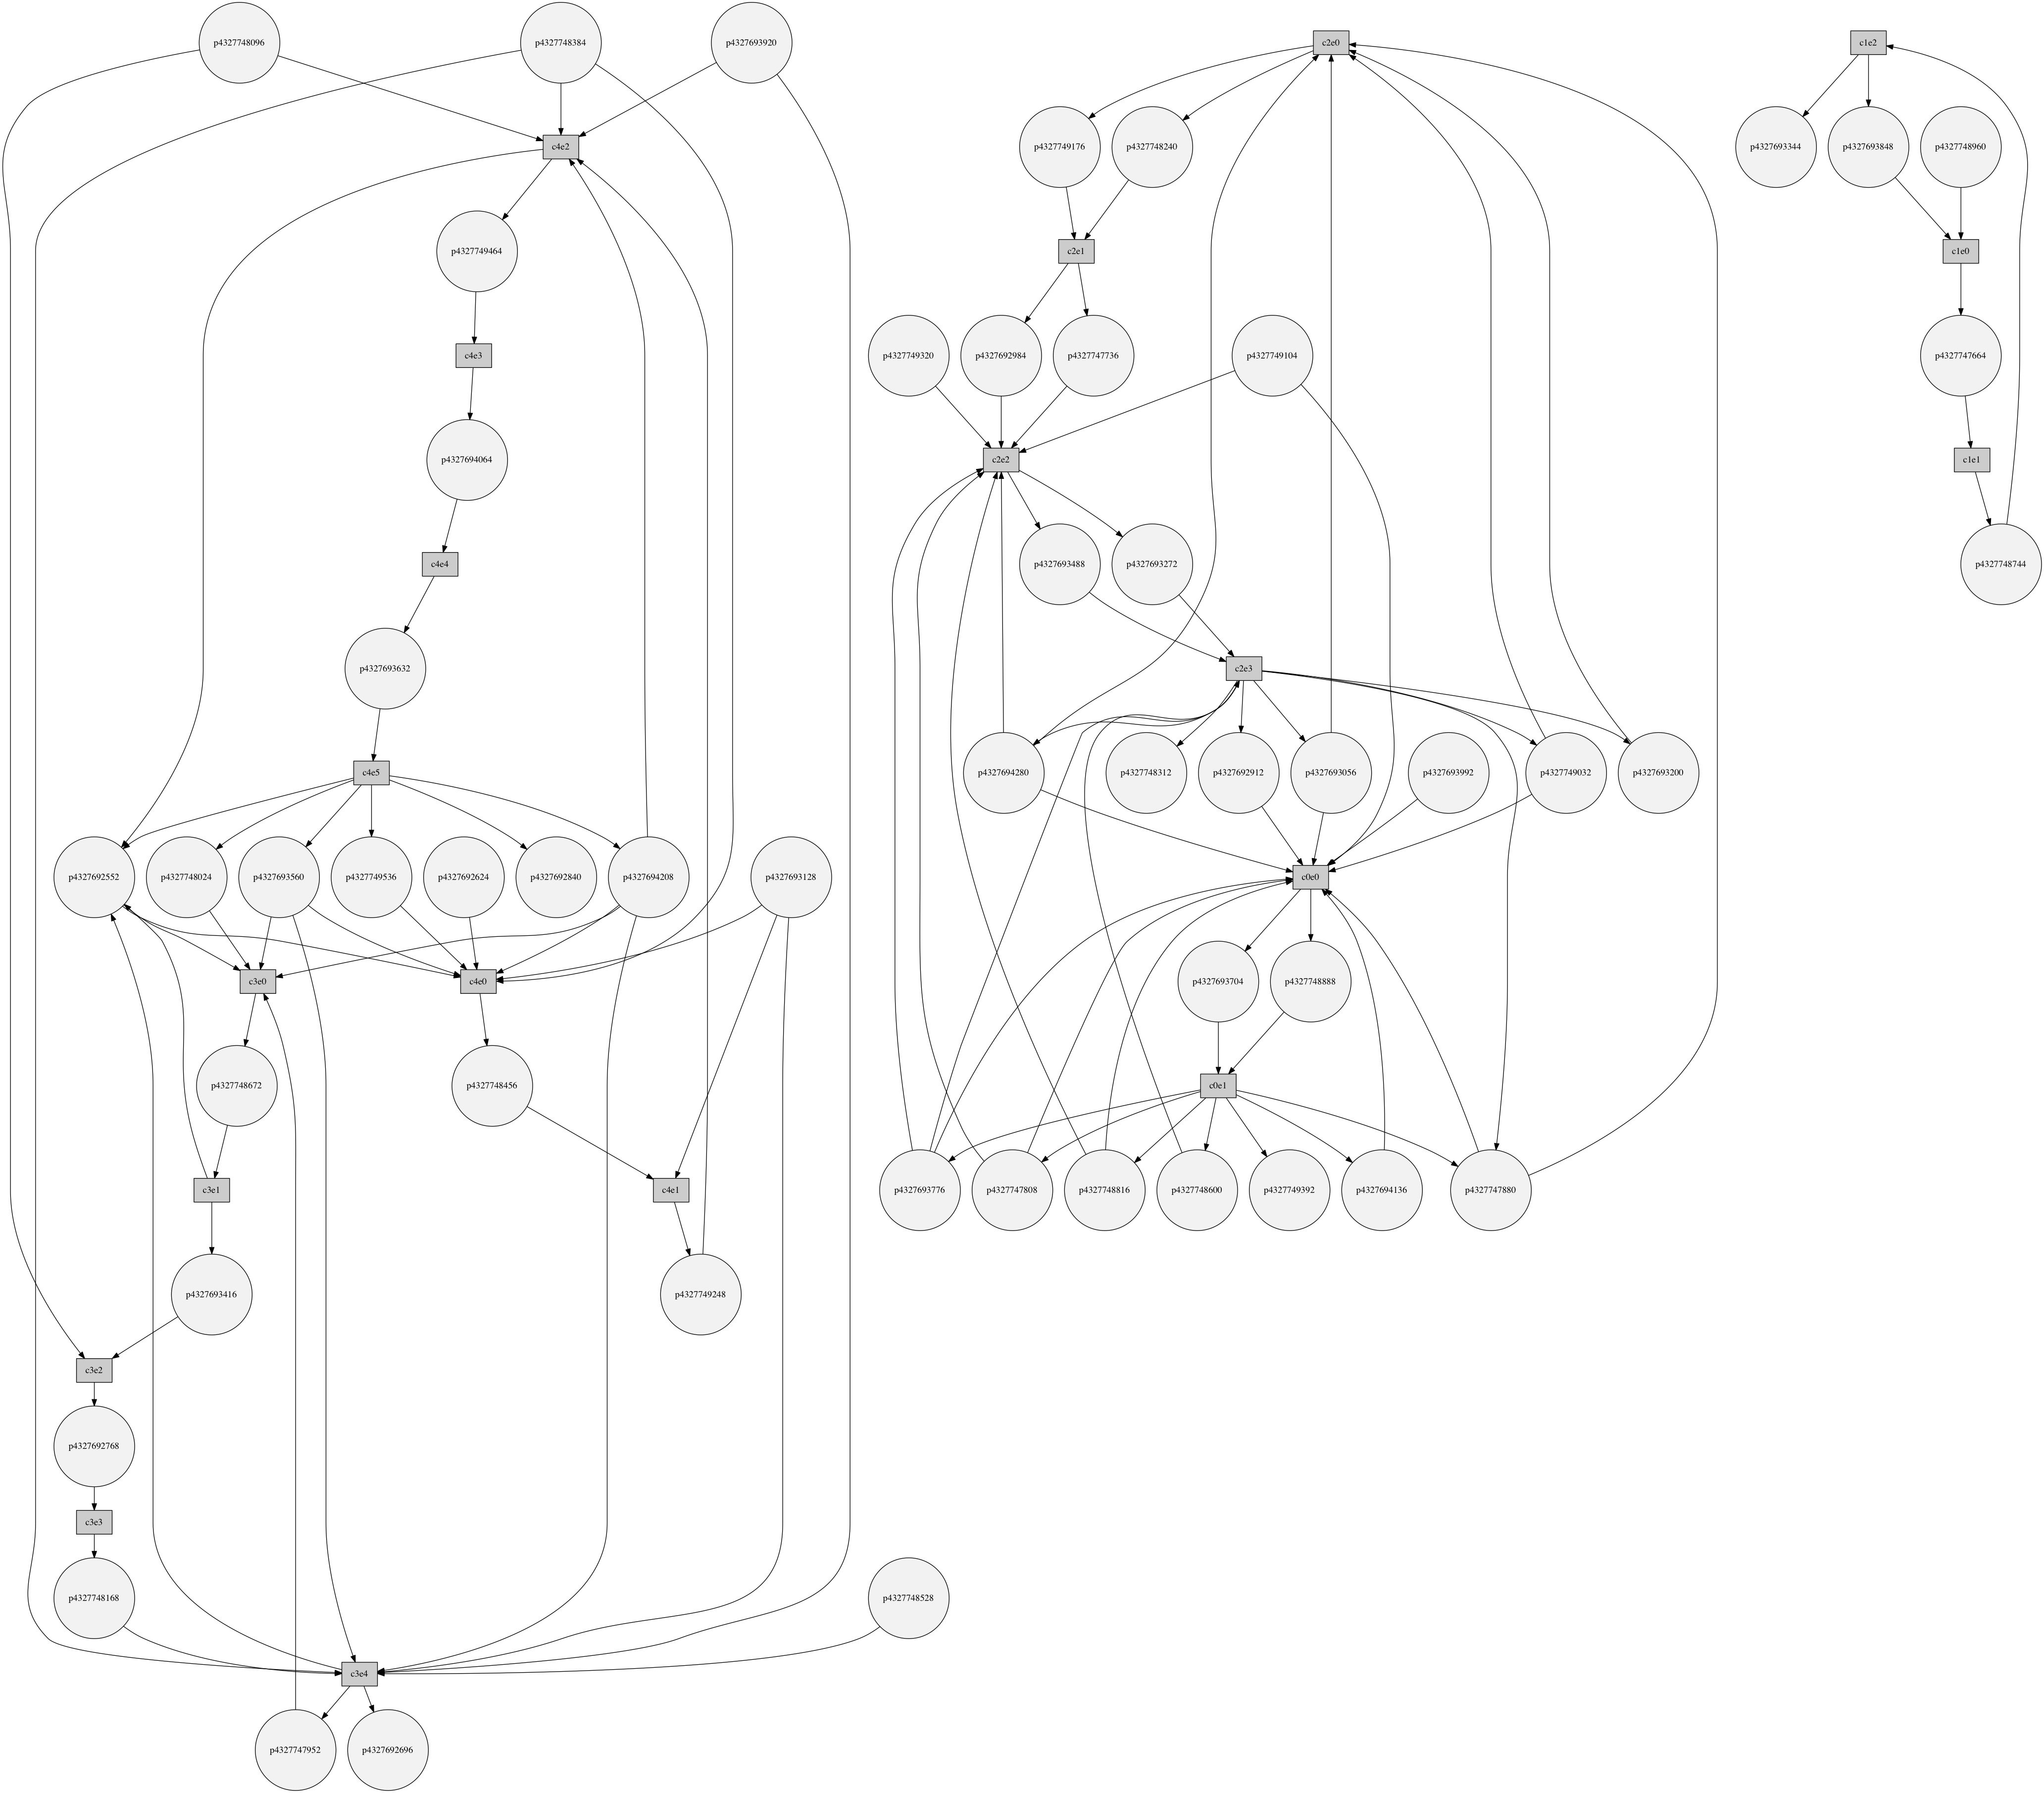
\includegraphics{img/cycles-pol}}}
%%%    \hspace{1cm}
%%%    \subbottom[\label{sfig:allsimp.2}\tiny\textsc{Removal} sobre~\autoref{sfig:allsimp.1}]{\scalebox{.05}{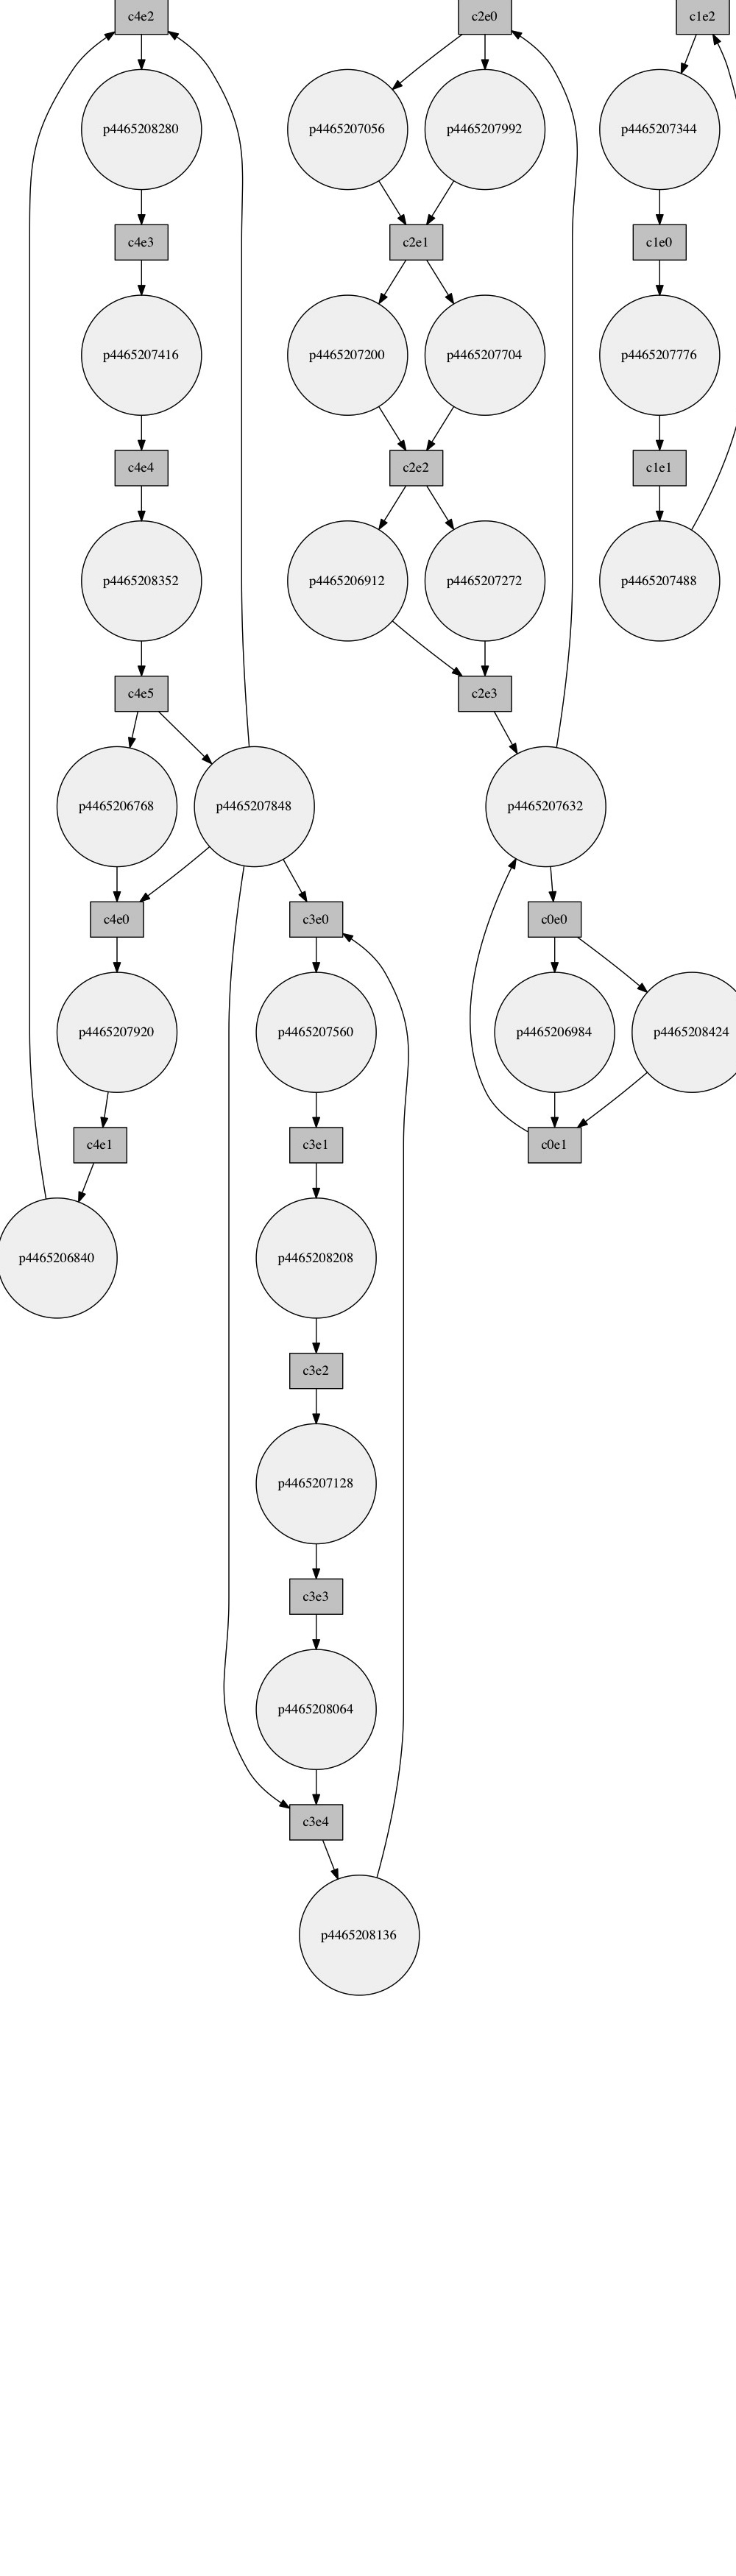
\includegraphics{img/cycles-pol-rem}}}
%%%    \subbottom[\label{sfig:allsimp.3}\tiny Enfoque de~\cite{Murata89}]{\scalebox{.04}{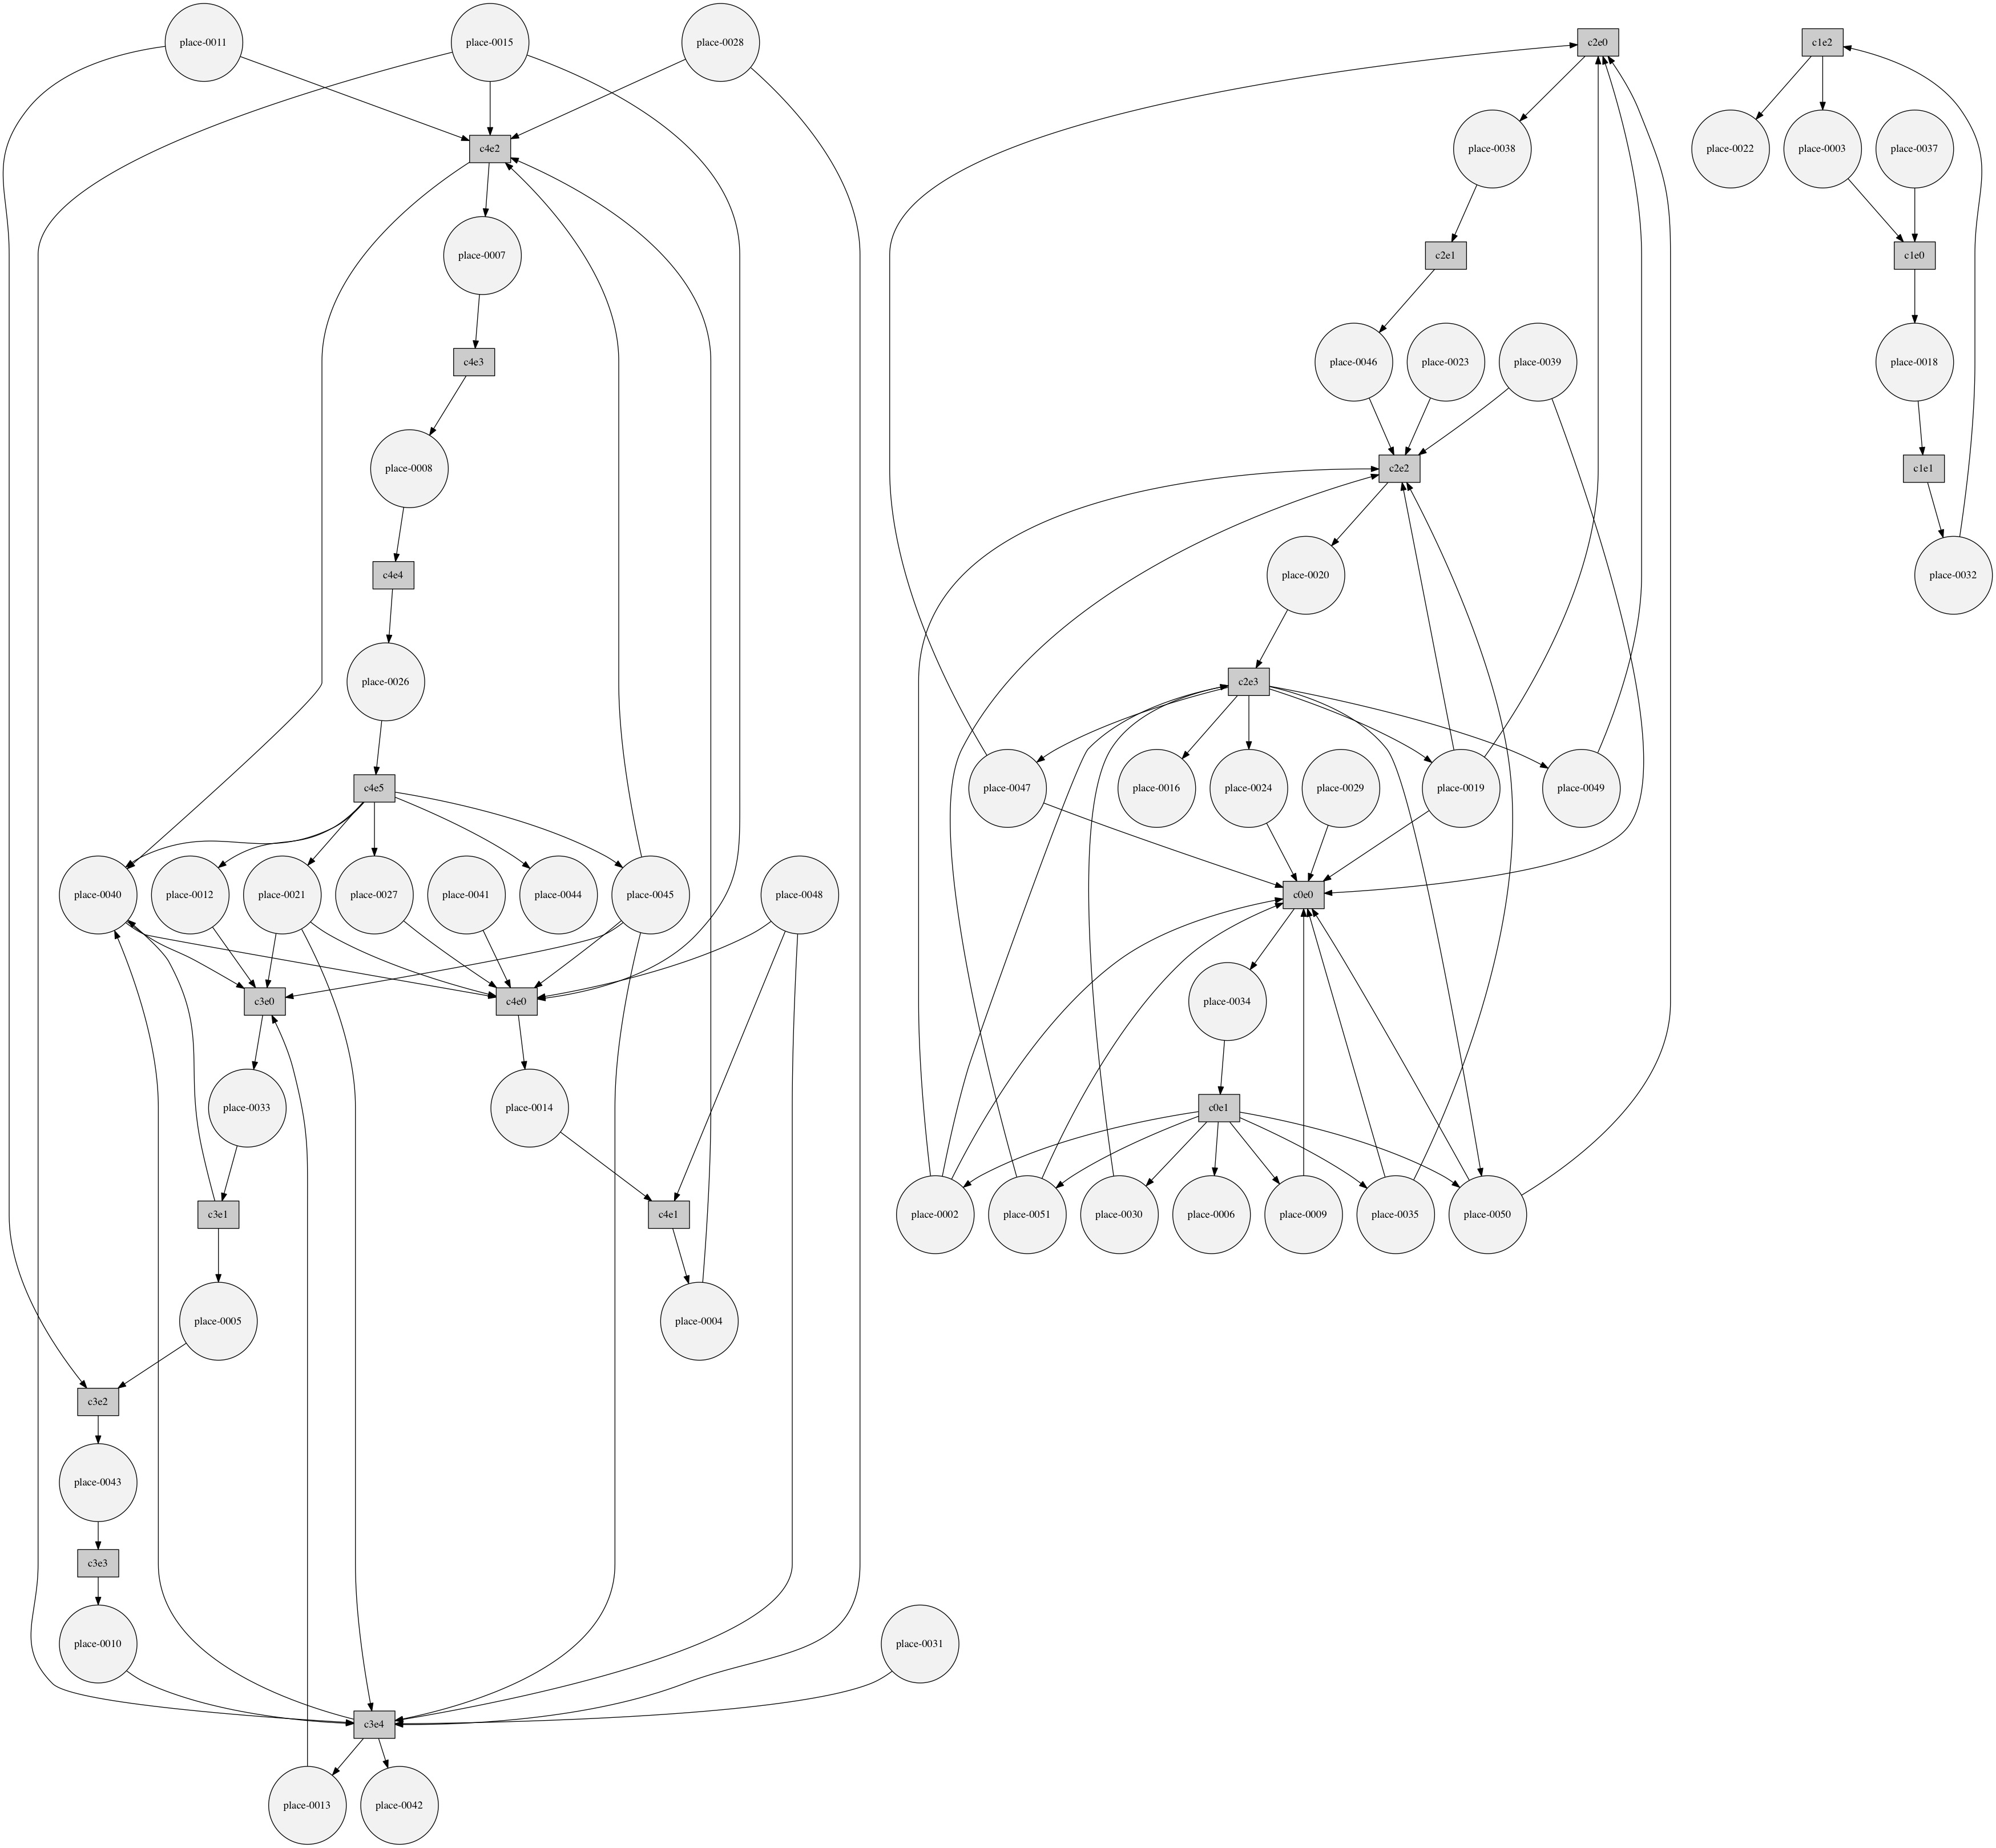
\includegraphics{img/cycles_murata}}}
%%%    \hspace{7mm}
%%%    \subbottom[\label{sfig:allsimp.4}\tiny Enfoque de~\cite{LeonCB15}]{\scalebox{.04}{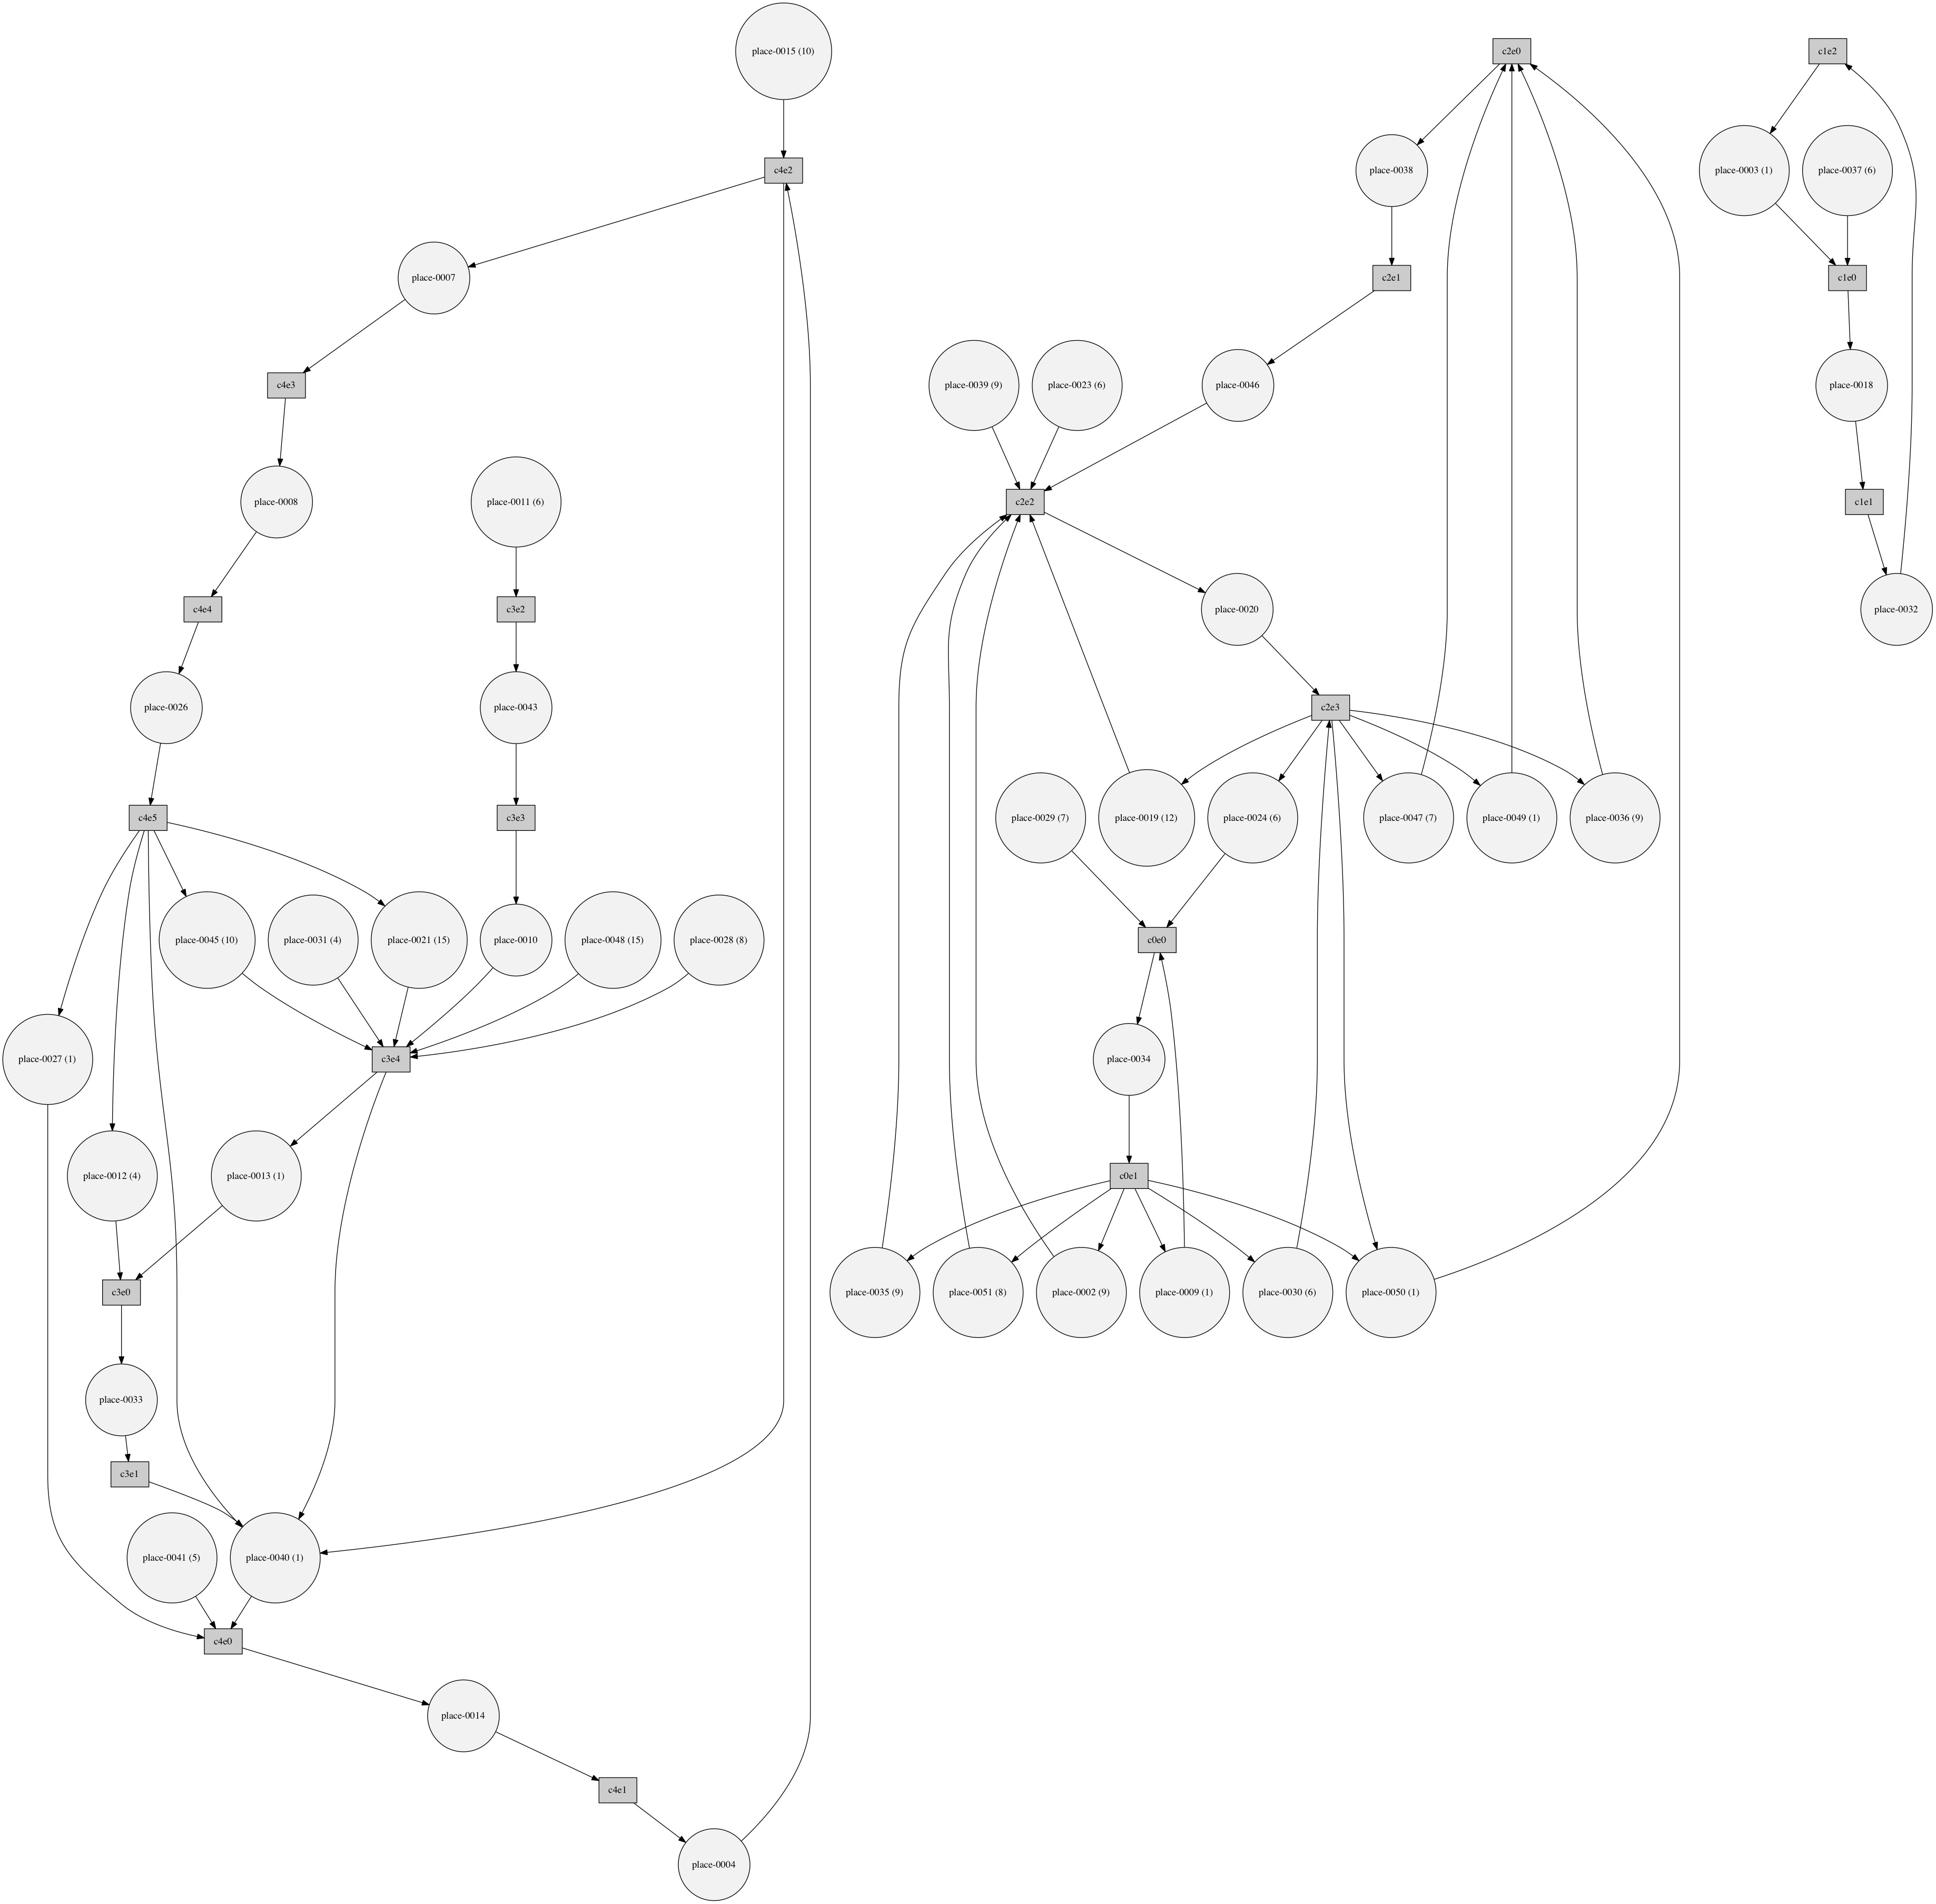
\includegraphics{img/cycles_pnsimp}}}
%%%    \caption{Ejemplo de la aplicación de la técnica presentada.}
%%%\end{figure}

\section{Alcance del trabajo}
\label{sec:alcance}

Esta tesina se plantea como una extensión superadora de los trabajos de Carmona y Cortadella en~\cite{CarmonaC14}
y de Ponce de León, Carmona y vanden Broucke en~\cite{LeonCB15}. 
Sin embargo, ambos enfoques poseen algunas restricciones las cuales son heredadas por esta tesina:
los logs de eventos de entrada del procedimiento deben ser libres de ruido -\textit{noise free}- y las redes generadas
por el proceso se limitan a redes de Petri puras (i.e. aquellas que no contienen ciclos de longitud uno).
Estas restricciones se deben al hecho de que se utiliza teoría de poliedros convexos directamente sobre el log de eventos.

Podrían evitarse estas limitaciones si se  pre-procesa el log de eventos, filtrando el ruido existente mediante
técnicas conocidas o bien puede incrementarse artificialmente la longitud de los ciclos de longitud uno evitando los modelos 
no puros. Sin embargo, estos procedimientos escapan del alcance de la tesina y se trabajará considerando las limitaciones
enunciadas.

\section{Estructura de la tesina}
\label{sec:estructura}

En este capítulo se presentaron las motivaciones y los objetivos principales para este trabajo el cual se
plantea como una extensión al trabajo realizado en~\cite{CarmonaC14} y~\cite{LeonCB15}.


Los siguientes capítulos del presente trabajo están organizado de la siguiente manera:

En el~\autoref{chap:2}, se introducen todas las nociones preliminares necesarias para comprender las contribuciones 
presentadas y plantea una formalización del problema a abordar.

La metodología utilizada para determinar el descubrimiento supervisado de procesos es presentado en el~\autoref{chap:3}, 
en donde se detallan los fundamentos teóricos de la técnica desarrollada y se muestra además, como puede utilizarse para simplificar
y generalizar modelos de procesos arbitrarios.

El~\autoref{chap:4} por su parte, presenta \pachtool, la herramienta desarrollada para esta tesina. Además en este mismo capítulo
se presentan los resultados experimentales de ejecutar \pachtool sobre diferentes benchmark, tanto como una herramienta de descubrimiento
supervisado de procesos así como también utilizándola como herramienta de post procesamiento sobre modelos arbitrarios.

Finalmente en el~\autoref{chap:5} se presentarán las conclusiones de esta tesina y se presetan una serie de posibles trabajos futuros.

\section*{Presentación en sociedad}
\label{sec:presentacion}

Los resultados teóricos de estas tesina resultaron en un artículo enviado al \dquote{Infomation System Journal} y se encuentra actualmente
en  proceso de revisión.

Adicionalmente, \pachtool compite en el primer \textit{Process Discovery Contest} cuyos resultados serán revelados durante la comferencia
BPM a desarrollarese en septiembre del corriente en Río de Janeiro.

% Nociones preliminares
% Capítulo 2 - Nociones preliminares
\chapter[Nociones preliminares]{Nociones preliminares}
\label{chap:2}

En este capítulo introduciremos las definiciones y conceptos básicos con los que se trabajará durante el desarrollo de esta tesina. Se presentarán las \textit{redes de Petri} (\autoref{sec:2.petrinets}), la \textit{minería de procesos} (\autoref{sec:2.process mining}), \textit{Parikh Vectors} (\autoref{sec:2.parikh}),
\textit{Domínios numéricos abstractos} y su aplicación al desubrimiento de procesos (\autoref{sec:2.discovery}) así como los conceptos utilizados de \textit{logs} (\autoref{sec:2.logs}) e \textit{información negativa} (\autoref{sec:2.negative}).
\\

Por último, utilizando estos conceptos, plantearemos de manera concreta el problema a resolver en los capítulos siguientes (\autoref{chap:2.problem}).

\section{Redes de Petri}
\label{sec:2.petrinets}
Las \textbf{redes de Petri}, introducidas en el año 1962 por el matemático
Carl Adam Petri, consisten en una generalización de la teoría de automátas.
Nacidas de la necesida de de representar sistemas dinámicos con eventos concurrentes;
forman un lenguaje gráfico y matemático con una semántica formal.
Desde su creación, han sido utilizadas para, entre otros usos, para representación,
análisis, verificación y simulación de sistemas a eventos discretos con comportamiento dinámico\cite{Murata89}.

Una red de Petri esta formada por dos componentes, la red propiamente dicha y un conjunto
de \dquote{fichas} asignados a ciertos nodos de la misma.

La primera de estas componentes consiste en un grafo bipartito dirigido ponderado,
cuyos nodos se separan en los conjuntos dijuntos 
llamados lugares -\textit{places}- y transiciones -\textit{transitions}-.
Los arcos del grafo se dirigen tanto de los places a las transitions como viceversa.

En el momento de graficar una red de Petri, los places, por los general, se
representan mediante círculos y las transiciones mediante cajas o, simplemente, barras.

La segunda componente de una red de Petri consiste en la asignación
de un número entero de fichas o marcas a cada uno de los places, 
utilizado para simular el comportamiento dinámico y concurrente del sistema.
A la distribución de estas marcas sobre cada uno de los places, se la denomina
\textit{marking} y corresponde al estado en el cual se encuentra en cada momento el sistema.
La distribución inicial de estas fichas, por tanto, se conoce como \textit{marking inicial}.

Gráficamente, esta asignación se representa de manera distribuída, indicando dentro 
de cada place el número entero asignado por el marking, o bien, dibujando una 
cantidad de puntos igual a dicho número.
\\

Formalmente, una red de Petri es una 4-upla $(P,T,F,M_0)$ donde $P$ y $T$\footnotemark[1]
representan los conjuntos finitos y disjuntos de places y transitions respectívamente.
Por su parte, las transiciones ponderadas vienen dadas por \mbox{$F:(P \times T) \cup (T \times P)  \to \nat$}
y un marking $M$ viene dado por la función \mbox{$M:P \to \nat$}.
En particular, llamamos $M_0$ al estado inicial de la red, i.e. el marking inicial.

\footnotetext[1]{ En este trabajo, utilizamos el mismo símbolo $T$ para denotar el conjunto de transiciones -\textit{transitions}-
    de una red de Petri así como para el alfabeto de eventos de las trazas de un log.
    
    Esta colisión es intencionada ya que, en nuestro modelo, cada transición se corresponde biunivocamente
    con una actividad del log (solo consideramos la actividad completa y no el inicio/fin como en otros enfoques).
    Por esta razón, las transiciones silenciosas (aquellas donde su ejecución no puede ser observada)
    no son admitidas en la red y por la cual dos transiciones diferentes no pueden representar una misma acción.
}

Denotamos el \textit{preset} y \textit{postset} de un place $p$ como $\preset{p}$ y $\postset{p}$ respectivamente,
los cuales se definen formalmente como: $\preset{p} =  \{t \in T ~|~ F(t,p) > 0 \}$
y $\postset{p} = \{t \in T ~|~ F(p,t) > 0 \}$.

Se le llama red de Petri \emph{pura} a una red que no posea ciclos de longitud uno, i.e.
$\forall p \in P:~ {\preset{p}} \mathrel{\cap} {\postset{p}} = \emptyset$.
En adelante, asumiremos que todas las redes de Petri con las que trabajamos son puras.
Esto es una consecuencia de utilizar la teoría de poliedros. Es importante destacar que esto no es una 
restricción importante ya que podemos, de manera sistemática, relajar un modelo no puro agregando
places ficticios y convertir cualquier lazo en un ciclo de longitud dos para obtener una red de Petri pura.
\\

Como notamos anteriormente, las redes de Petri se utilizan para representar sistemas 
dinámicos; este comportamiento dinámico está definido mediante las \emph{reglas de evolución}.

Decimos que una cierta transición $t \in T$ esta \emph{habilitada},
en un cierto marking $M$ si \mbox{$\forall p \in P, M(p) \ge F(p,t) $}.

Ejecutar una transición $t$ en un marking induce un nuevo marking $M'$
definido de manera incremental, como  \mbox{$M'(p) = M(p) - F(p,t) +  F(t,p)$},
para cualquier $p \in P$. A esta evolución la notamos \firing{M}{t}{M'}.

Una cierta secuencia de transiciones \mbox{$\sigma = t_1,t_2, t_3, \ldots, t_n$}
se dice ejecutable si existe una secuencia de markings \mbox{$\omega = M_1, M_2, \ldots, M_n$}
tal que ocurra la evolución
\firing {\firing {\firing {\firing {M_0} {t_1} {M_1}} {t_2} {M_2} } {t_3} {\cdots}} {t_n} {M_n}.

Dada una red de Petri $N$, llamamos $\Language(N)$ al lenguaje de la misma, i.e.
el conjunto de secuencias de transitions ejecutables sobre $N$.
Por su parte, al conjunto de markings alcanzable partiendo desde el marking inicial $M_0$,
llamado \emph{conjunto alcanzable} de $N$, lo notamos $\rs(N)$.

\begin{figure}[t]
  	\centering
    \begin{tikzpicture}

  \node[transition] (x) at (-.75,-1) {$x$};
  \node[transition] (y) at (.75,-1) {$y$};
  \node[tplace,label=above:$p_1$] (p1) at (0,0) {};
  \node[tplace,label=below:$p_0$] (p2) at (0,-2) {};
      
  \node[] (t) at (p1) {6};
  \node[] (t) at (p2) {1};
    
  \draw[style={->,>=triangle 45}] (p1) edge node[above left]{2} (x);
  \draw[style={->,>=triangle 45}] (x) to (p2);    
  \draw[style={->,>=triangle 45}] (p2) to (y);      
  \draw[style={->,>=triangle 45}] (y) edge node[above right]{3} (p1);
  
  \node[] (null) at (0,-3) {};
  
\end{tikzpicture}

    \caption{Una red de Petri (pura) con pesos no unitarios.}
    \label{fig:pn1}
\end{figure}

Consideremos ahora un place $p$ con
\mbox{$\preset{p}=\{x_1,\ldots,x_k\}$},
\mbox{$\postset{p}=\{y_1,\ldots,y_l\}$} y una función de transición 
$F$ igual a la función constante 1.
Siendo $M_0(p)$ la cantidad de tokens en el marking inicial 
para el place $p$, entonces, la siguiente ecuación
se satisface para cualquier secuencia de eventos $\sigma$

\beql{1place_cte}
M(p) = M_0(p) + \widehat\sigma(x_1)+\cdots +\widehat\sigma(x_k) -
\widehat\sigma(y_1)-\cdots -\widehat\sigma(y_l).
\eeq

La ecuación \eqref{eq:1place_cte}, puede generalizarse para permitir arcos
ponderados como

\beql{1place_wei}
M(p) = M_0(p) + \sum_{x_i \in \preset{p}}F(x_i,p)\cdot
\widehat\sigma(x_i) -
\sum_{y_i\in\postset{p}}F(p,y_i)\cdot\widehat\sigma(y_i).
\eeq

Si extendemos \eqref{eq:1place_wei} a todos los places de una red de Petri,
utilizando la notación matricial, tenemos

\beql{matrix_eq}
M = M_0 + A \cdot \widehat\sigma 
\eeq

donde $M$ y $M_0$ son vectores y $A$ representa la \emph{matriz de incidencia}
del grafo; $A$ posee $|P|$ filas y $|T|$ columnas y representa las conexiones 
existentes en la red.
A la ecuación \eqref{eq:matrix_eq}, se la llama \emph{ecuación de marking} de una red
de Petri~\cite{Murata89}.

Ademas, llamamos \emph{conjunto potencialmente alcanzable}
al conjunto de soluciones de la siguiente ecuación

\beql{matrix_ineq}
M = M_0 + A \cdot \widehat\sigma \geq 0
\eeq

y lo notamos $\prs(N)$.
Utilizando la ecuación \eqref{eq:matrix_ineq} resulta simple definir el concepto
de complejidad de una red de Petri que utilizamos. El mismo consiste en la suma
de los valores absolutos de todos los coeficientes de la matriz $A$ con la suma
de los valores absolutos del vector de $M_0$.

A continuacion, a modo de ejemplo, construímos la ecuación \eqref{eq:matrix_ineq} de
la red de Petri de la ~\autoref{fig:pn1}, la cual es

\beq
 \left[\begin{array}{c} 1 \\ 6 \end{array} \right] +
\left[\begin{array}{rr} 1 & -1 \\ -2 & 3 \end{array} \right]
\cdot
\left[\begin{array}{c} \widehat\sigma(x) \\ \widehat\sigma(y) \end{array}
\right]
\geq \left[\begin{array}{c} 0 \\ 0 \end{array} \right]
\eeq

Es importante ver que todo marking alcanzable de una red de Petri
satisface \eqref{eq:matrix_ineq}, sin embargo, lo opuesto no siempre es cierto.
En general, pueden existir markings no alcanzables para
los cuales \eqref{eq:matrix_ineq} se satisface, i.e. $\rs(N) \subseteq \prs(N)$.

\section{Minería de procesos} 
\label{sec:2.process mining}

\subsection{Logs} 
\label{sec:2.logs}

La minería de procesos tiene su punto inicial en la recopilación de una serie de \textit{log de eventos}. 
Un evento refiere a una actividad, observable o no, de un proceso y
un log de enventos -o simplemente \textit{log}- se define como una secuencia
ordenada de estos eventos, por lo general, generadas de manera automática.
Un log corresponde a una instancia única de la ejecución de un sistema, llamada, instancia de proceso o caso y 
durante la minería de procesos, suelen utilizarse varíos casos de sobre un mismo proceso.

Un log posee los siguientes elementos constitutivos fundamentales: un conjunto de actividades,
un cierto orden temporal en el cual ocurren y un caso o instancia de proceso que agrupe dichas actividades.
Sin embargo, un log pueden contener, además, datos adicionales que, aunque no sean fundamentales, pueden
ayudar a la minería de procesos otorgándole mayor nivel de detalle y claridad.

La tabla \autoref{tab:log_ex} muestra un ejemplo parcial de un conjunto de logs con información adicional (i.e. medio, actividad, nivel) que permite un entendimiento mayor del devenir del proceso,

\begin{table}[t]
\tiny

\def\sep{\hspace{10pt}}
\begin{tabular}{r   c   l   l   r   c   c}
  \tiny \#Caso
& \tiny Timestamp
& \tiny Medio
& \tiny Tipo
& \tiny Urgencia
& \tiny Usr
& \tiny Grupo
\\
\midrule
 970 & 2015-12-31 23:55:12 & Teléfono & Aviso & 0 & Andrés & Nivel 1\newrow
 970 & 2015-12-31 23:56:22 & Mail & Reclamo & 0 & Andrés & Nivel 1\newrow
 970 & 2016-01-01 00:05:11 & Teléfono & Reclamo & 1 & Andrés & Nivel 1\newrow
 971 & 2016-01-01 00:30:44 & Mail & Abierto & 2 & Gonzalo & Nivel 1\newrow
 971 & 2016-01-01 00:30:44 & Mail & Resuelto & 2 & Gonzalo & Nivel 1\newrow
 970 & 2016-01-01 00:30:44 & Teléfono & Derivado & 0 & Andrés & Nivel 2\newrow
 312 & 2016-01-01 15:30:01 & Mail & En progr. & 3 & Gonzalo & Nivel 3\newrow
 42 & 2016-05-04 00:00:01 & Mail & Resuelto & 10 & Lucio & Nivel x\newrow
 42 & 2016-05-04 00:00:01 & Mail & Resuelto & 10 & Lucio & Nivel x\newrow
 $\vdots$ & $\vdots$ & $\vdots$ & $\vdots$ & $\vdots$ & $\vdots$ & $\vdots$ \newrow
\end{tabular}
\vspace{0pt}
\caption{\tiny Un ejemplo artificial de un log de eventos con información adicional.}
\label{tab:log_ex}
\end{table} 


Formalmente, dado un alfabeto $T$\footnote{Ver nota previa referente a la colisión de nombres} representando
al conjunto de posibles eventos, un log se define como un conjunto $\pmlog \in \mathcal{P}(\eventstar)$\footnote{
Los logs pueden ser definidos de manera más general como multiconjuntos donde algunos comportamientos
pueden ser observados múltiples veces. No consideramos este enfoque ya que no consideramos 
la frecuencia de cada traza; las redes solo contemplan la presencia o ausencia de un cierto comportamiento.}. 


Los elementos del log \pmlog, llamados \textit{trazas}, son secuencias de eventos de $T$,
i.e. $\sigma \in \eventstar$.
Dados un numero natural $1 \leq k \leq n$ y una traza $\sigma=\sigma_1,\sigma_2,\dots,\sigma_n$, a la traza
$\sigma_1,\sigma_2,\dots,\sigma_k$ se la llama prefijo -\textit{prefix}- de $\sigma$.

Abusando de notación,  si una cierta traza $\sigma'$ es el prefijo de alguna traza de $\pmlog$, se dice que 
$\sigma' \in \pmlog$ .

% The problem of process discovery requires the computation of a model $\model$ that adequately represents
% a log $\pmlog$.
% A model $\model$ is {\em overfitting} with respect to log $\pmlog$ if it is too specific and too much driven
% by the information in $\pmlog$. On the other hand, $\model$ is an {\em underfitting} model for $\pmlog$ if the behavior
% of $\model$ is too general and allows for things ``not supported by evidence'' in $\pmlog$.  Whereas overfitting
% denotes lack of generalization, underfitting represents too much generalization. A good balance between
% overfitting and underfitting is a desired feature in any process discovery algorithm~\cite{AalstBook}. There exists several formalism for modeling
% processes; those include transition systems, workflow nets, BPMN and causal nets between others. In this article we will discover processes modeled
% as Petri nets.

\subsection{Minería de procesos} 
\label{sec:2.process mining subsection}

Process discovery techniques aim
at extracting from a log $\pmlog$ a process model $N$ (e.g., a Petri net) with the goal to elicit the process
underlying in ${\sys}$. By relating the behaviors of $\pmlog$, $\Language(N)$ and ${\sys}$,
particular concepts can be defined~\cite{BuijsDA14}. A log is \emph{incomplete} if ${\sys} \setminus \pmlog \ne
\emptyset$. A model $N$ \emph{fits} log $\pmlog$ if $\pmlog \subseteq \Language(N)$. A model is
\emph{precise} in describing a log $\pmlog$ if $\Language(N) \setminus \pmlog$ is small. A model $N$
represents a \emph{generalization} of log $\pmlog$ with respect to system ${\sys}$ if some behavior in ${\sys}
\setminus \pmlog$ exists in $\Language(N)$. Finally, a model $N$ is \emph{simple} when it has the minimal
complexity in representing $\Language(N)$, i.e., the well-known \emph{Occam's razor principle}.
It is widely acknowledged that the size of a process model is the
most important simplicity indicator~\cite{AalstBook}. However, as we will see in Section~\ref{sec:ssr}, this paper introduces
a tailored simplicity metric which is sensitive to the type of models considered.

\section{Parikh Vector} 
\label{sec:2.parikh}

\section{Domínios númericos abstractos y descubrimiento de procesos} 
\label{sec:2.discovery}

\section{Información negativa} 
\label{sec:2.negative}

\section{Enunciado del problema} 
\label{sec:2.problem}

Dado un log $\pmlogp$ y un conjunto de trazas negativas $\pmlogn$ el objetivo de las técnicas utilizadas 
en el desarrollo de la tesina es derivar $N$ tal que posea las siguientes caraterísticas:\\

\begin{itemize}
 \item $N$ es una red de Petri pura ponderada;
 \item $\forall \sigmap \in \pmlogp:~ \sigmap \in \Language(N)$;
 \item $\forall \sigman \in \pmlogn:~ \sigman \notin \Language(N)$;
 \item $N$ minimiza su complejidad. 
\end{itemize}

Los primers tres items son triviales ya que son garantizados por la metodología utilizada
para generar la red.

\todo[inline]{traducir el texto que sigue.}
, while for simplicity we will evaluate derived models with respect to a tailored fine-grain simplicity metric
which takes into account not only the number of elements but also its weight. In the evaluation section, we will use current metrics for precision and
generalization to estimate whereas the derived models are in good balance between underfitting and overfitting the log.
\todo[inline]{Primero debería entenderlo....}

\section{Resumen del capítulo}
\label{sec:2.resumen}
En este capítulo se hizo una introducción a diferentes temas fundamentales para la comprensión y el desarrollo de este trabajo. 
Se presentaron conceptos cruciales como \textit{redes de Petri} y \textit{minería de procesos}, definiciones como la
de \textit{Parikh Vector} y se describireron las nociones utilizadas de \textit{logs}, \textit{información negativa} o el concepto 
entendido por complejidade de una red de Petri.
\todo[inline]{rellenar el resumen del capítulo}
En particular, 
\todo[inline]{rellenar el resumen del capítulo. Primero sería bueno terminarlo para contar que dice, no?}
Por último, utilizando estos conceptos, se presentó una definición formal del problema a tratar.

% Descubrimiento de procesos supervisado
\chapter{Descubrimiento de procesos supervisado}
\label{chap:3}

En este capítulo, nos centraremos en el área de la minería de procesos que refiere
al descubrimiento de procesos. Como vimos, el descubrimiento de procesos busca un modelo 
que represente el funcionamiento de un cierto sistema a partir de un log del mismo.
Para ello, revisamos el algoritmo de descubrimiento introducido en~\cite{LeonCB15},
el cual consiste en una extensión del algoritmo en~\cite{CarmonaC14} que permite 
introducir información negativa al proceso de búsqueda. De este análisis se observan 
ciertas limitaciones que poseen estos enfoques, por lo cual planteamos un nuevo 
algoritmo de descubrimiento como una extensión al proceso en~\cite{LeonCB15} mediante 
la que buscamos salvar ambos inconvenientes con el fin de obtener, de manera automática, 
un modelo que sea a la vez adecuado, preciso, general y simple.

Se detallará el algoritmo de descubrimiento propuesto y se mostrará además,
que la técnica introducida es independiente del proceso de descubrimiento
y puede ser utilizado para simplificar los modelos obtenidos por otras técnicas 
de descubrimiento de procesos.

\section{Algoritmo de descubrimiento}
\label{sec:3.algodisco}

Según lo visto en \autoref{sec:2.discovery discovery}, el descubrimiento de procesos
refiere al proceso mediante el cual, partiendo del log de un sistema, se busca
un modelo que lo represente.
Para este fin, existen diferentes metodologías~\cite{CarmonaC14,LeonCB15,MedeirosAW03,AalstWM04}.
En este trabajo, se introduce una extensión del algoritmo presentado en~\cite{LeonCB15} (el cual a
su vez consiste en una extensión de~\cite{CarmonaC14}). Este algoritmo posee algunas falencias
que se detallan a continuación.

El primer inconveniente, proveniente del enfoque utilizado en~\cite{CarmonaC14}, 
surge del crecimiento exponencial de su complejidad con respecto al número de actividades 
en un log: se introduce una estrategia del tipo \dquote{divide y vencerás}, 
utilizando proyección -\textit{projection}- así como el concepto de muestreo -\textit{sampling}-.
Las técnicas de muestreo y proyección, conforman una solución satisfactoria al problema del
crecimiento exponencial, pero al mismo tiempo, la calidad de las métricas referentes a 
precisión y simplicidad suelen ser degradadas considerablemente generando un modelo complejo
que admite demasiados comportamientos además de los observados en el log, 
i.e. se obtiene un modelo \textit{overfitting}.

\begin{remark}[Projection]
    \textit{Projection} hace referencia al principal método utilizado para aliviar la carga
    computacional inherente al algoritmo de descubrimiento utilizado, cuya complejidad
    crece exponencialmente en relación a los puntos del conjunto de vectores Parikh de un cierto
    log. Projection es un método del tipo divide y vencerás que consta de tres partes. 
    La primera se ocupa de agrupar los eventos del log en grupos -\textit{clusters}-
    para los cuales existe un alto grado de correlación. 
    Luego se resuelve el problema de manera aislada para cada uno de los grupos.
    Por último, se buscan relaciones entre los diferentes grupos de manera de 
    conectar las diferentes soluciones de los subproblemas en lo que será
    el modelo final del problema.
\end{remark}

\begin{remark}[Sampling]
    \textit{Sampling} corresponde a una técnica utilizada para hacer factible utilizar
    logs de gran tamaño, lo cual es usual.
    Obtener la cápsula convexa posee un alto costo computacional, por lo que, sí el log utilizado
    como argumento es de gran tamaño, lo hace impracticable.
    Mediante sampling lo que se hace es seleccionar de manera aleatoria un subconjunto de los
    puntos del conjunto de vectores Parikh correspondiente al log como entrada para calcular y 
    luego se filtran aquellos resultado obtenidos, eliminando aquellos que no admitan alguno 
    de los puntos iniciales.
\end{remark}

\begin{example}
    Sea el log $\pmlog=\{ ac, abac, abab \}$ cuyo vector de Parikh es 
    $\parikh{\pmlog}=\{ (0,0,0),(1,0,0), (1,0,1),\\(1,1,0), (2,1,0), (2,1,1),(2,2,0) \}$ (asumiendo el orden $(a,b,c)$).
    Si se proyecta sobre las actividades $\{a,b\}$ y se utiliza una muestra con los puntos
    $\{(1,0,1),(1,1,0),(2,1,1),(2,2,0)\}$, el conjunto de puntos proyectados es
    $\{ (1,0), (1,1), (2,1), (2,2) \}$. 
    Así, utilizando las técnicas en~\cite{CarmonaC14}, se obtendrá un modelo con
    representado por la inecuación \mbox{$a \ge b$}.
    
    Puede observarse que esto representa una subestimación del modelo ideal (si se consideran
    todos los puntos del log), el cual puede representarse mediante la inecuación $a \ge b + c$.
\end{example}

La segunda limitación surge de la metodología utilizada para computar el poliedro que contiene los 
puntos en el conjunto de vectores de Parikh. Debido a la metodología utilizada, se obtiene un 
modelo complicado del sistema. Debido a la metodología utilizada, se obtiene un 
modelo complicado del sistema. Existe en~\cite{CarmonaC14} un post procesamiento de simplificación, pero este es
realizado de manera heurística y manual, seleccionando un subconjunto de las restricciones que conforman la
$H$-representación del poliedro computado. Solo se utilizan las restricciones con coeficientes \dquote{simples}, 
eliminando el resto del modelo. 
Esta elección esta basada en la presunción de que, en la vida real, los procesos son definidos de manera
que sean \textit{simples} y más especialmente en el campo de la gestión de procesos de negocio. Esta presunción,
aunque no es necesariamente desacertada, generalice demasiado el modelo, convirtiéndolo en un modelo
impreciso.

Por su parte, en~\cite{LeonCB15} se propone un método supervisado para la simplificación del modelo que 
introduce el manejo de información negativa en caso de estar disponible.
De manera iterativa, se consideran cada uno de los hiperplanos que conforman la $H$-representación del poliedro
y se intenta desplazar y rotar el mismo para obtener un modelo más simple.
Para evitar degradar el sistema, al simplificar cada inecuación se limita de manera que cada punto aceptado
inicialmente siga siendo aceptado y, en caso de poseer información negativa, se restringe la simplificación
de manera que ningún punto prohibido sea aceptado.

El inconveniente con este enfoque es que trata los hiperplanos de manera aislada; cada inecuación
simplificada debe incluir, al menos, las mismas soluciones que la original (para evitar un modelo no adecuado) y no
debe incluir ningún punto negativo. Sin embargo, dado que el comportamiento del sistema no es definido por los 
semiespacios aislados sino por la unión de todos ellos, es el modelo quien no debe admitir puntos prohibidos 
y no un semiespacio particular.

\begin{example}
    \label{ex:prob_gen}
    En la \autoref{fig:glob_encoding}, se muestra un poliedro inicial \autoref{sfig:glob_encoding.1} 
    y un punto $(9,4)$ que pertenece al semiespacio definido por el plano $p$.

    \begin{figure}[H]
      \centering
      \subbottom[\label{sfig:glob_encoding.1}]{%
        \scaledinput{0.40}{img/ineq1}}
      \hfill
      \subbottom[\label{sfig:glob_encoding.2}]{%
        \scaledinput{0.40}{img/ineq2}}
      \caption{Simplificación individual vs. simplificación matricial.}
      \label{fig:glob_encoding}
    \end{figure}

    Si se aplica la técnica propuesta en~\cite{LeonCB15} a este plano, de manera aislada,
    no se obtendrá nunca el poliedro $p'$ en \autoref{sfig:glob_encoding.2} ya que
    $p'$ no admite como solución al punto $(9,4)$. 
    Sin embargo, es claro que el punto $(9,4)$ no pertenece al poliedro~\autoref{sfig:glob_encoding.2}.
\end{example}

\subsection{Etapas del procedimiento propuesto}
\label{sec:3.algodisco stages}

El procedimiento propuesto para descubrimiento y simplificación de procesos se ilustra en~\autoref{fig:flow}.
En la parte superior, dentro del marco negro, se representa el enfoque utilizado en~\cite{CarmonaC14} 
mediante el cual se obtiene un modelo sin utilizar trazas negativas; corresponde a la interpretación
de un log como un conjunto de vectores Parikh, luego la obtención de un poliedro y por ultimó a la 
transformación a una red de Petri según se detalló en~\autoref{sec:2.discovery}.

\begin{figure}[H]
    \begin{center}
%\scalebox{1}{\input{img/flow.pdf_t}}
    \scalebox{.6}{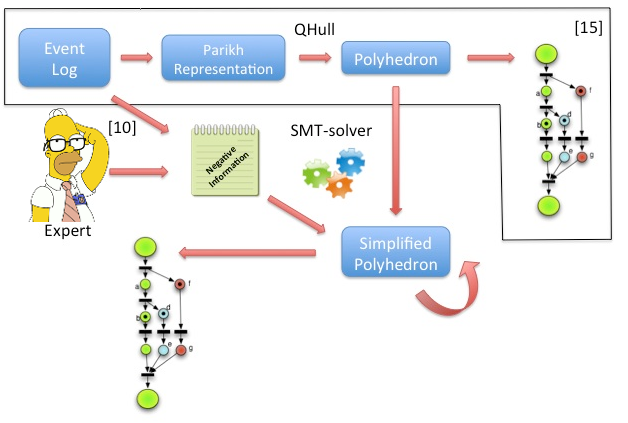
\includegraphics{img/approach_homero}}
    \caption{Procedimiento supervisado propuesto (fuera del marco) en contraposición al enfoque
        en~\cite{CarmonaC14} (dentro del marco).}
    \label{fig:flow}
    \end{center}
\end{figure}

Por otro lado, en la sección inferior de la \autoref{fig:flow}, se representa a modo de introducción,
como el uso de información negativa proveniente de diferentes medios, se utiliza para simplificar 
el modelo obtenido con el costo de incluir nuevos puntos al modelo final.
Los detalles de este enfoque se encuentran a continuación.

\begin{algorithm}[H]
\caption{Descubrimiento de procesos supervisado}
  \begin{algorithmic}[1]
      \Require trazas positivas $\pmlog^+$ y trazas negativas $\pmlog_-$
      \Ensure una red de Petri $N$ donde $\forall \sigma \in \pmlog^+: \sigma \in L(N)$ y $\forall \sigma \in \pmlog_-: \sigma \not \in L(N)$
      \vspace{1pt}
      \Procedure{DISCOVER}{$\pmlog^+, \pmlog_-$}
      \State $pp, np \leftarrow \emptyset$ \label{algo:line1}
      \For{$\sigma_p \in \pmlog^+$}
        \For{$\sigma$ prefix of $\sigma_p$}
          \State add $\widehat\sigma$ to $pp$
       \EndFor
     \EndFor
      \For{$\sigma_n \in \pmlog_-$}
        \State add $\widehat\sigma_n$ to $np$
      \EndFor \label{algo:line2}
      \State $H$ = \textsc{ConvexHull}($pp$) \label{algo:lineqhull}
      \State $H_{smt}$ = \textsc{Shift\&Rotate}($H, np$)
      \State $H'$ = \textsc{Removal}($H_{smt}, np$)
      \State $N$ = \textsc{Hull2Net}($H'$)
      \State \Return N
      \EndProcedure
  \end{algorithmic}
  \label{algo}
\end{algorithm}

El \autoref{algo} describe el enfoque propuesto paso a paso utilizando pseudocódigo. Un conjunto de trazas 
positivas y un conjunto de trazas negativas conforman la entrada 
(respectivamente \dquote{log de eventos} e \dquote{información negativa} en \autoref{fig:flow}). 
En las líneas \ref{algo:line1}-\ref{algo:line2} se calculan todos los puntos positivos $pp$ para
cada prefijo de una traza positiva en $\pmlogp$ y los puntos negativos $np$ para las trazas en $\pmlogn$\footnotemark[1].
Luego, se calcula un poliedro que contenga el conjunto de puntos $pp$ mediante \textsc{ConvexHull} utilizando 
métodos de programación lineal para obtener la cápsula convexa, e.g. \qhulltool~\cite{Barber96}.

El poliedro que se obtiene es luego simplificado de manera supervisada mediante la función 
\textsc{Shift\&Rotate} utilizando SMT-solvers. El resultado que se obtiene de un SMT-solver es 
una instancia de SMT, la cual no necesariamente provee la solución óptima (pueden existir múltiples soluciones), 
por lo que se utiliza un proceso de refinamiento iterativo para conseguir el óptimo.

La función \textsc{Removal} corresponde a la optimización del procedimiento de eliminación presentado en~\cite{LeonCB15}.
En este punto, se considera la información negativa $np$, eliminando únicamente aquellos hiperplanos
que no agreguen ninguno de los puntos de $np$ al modelo.

Por último, el conjunto de semiespacios es transformado en una red de Petri mediante \textsc{Hull2Net} utilizando
la dualidad que existe entre los poliedros y las ecuaciones de marking de una red de Petri
presentada en \autoref{sec:2.discovery discovery}.

Del hecho de que \textsc{ConvexHull} puede depender de las técnicas de muestreo y proyección y del
hecho que que \textsc{Shift\&Rotate} está representado como una instancia de SMT (la cual puede poseer múltiples soluciones
y la devuelta depender de la implementación del solver) el algoritmo \autoref{algo} es no determinista, i.e. dados
los mismos logs positivo y negativo de entrada se pueden obtener diferentes resultados.

\footnotetext[1]{ Nótese que en el caso de las trazas negativas, se utilizan únicamente los puntos correspondientes
    a cada traza completa y no a todos sus prefijos. Esto se debe a que para la mayor parte de las trazas negativas 
    el prefijo es compartido con alguna traza positiva por lo que no deben evitarse.
}
    
\section{Generalización y simplificación}
\label{sec:3.gensimp}

En la \autoref{sec:2.discovery} se explica como partiendo de un conjunto de logs de un sistema, se puede
buscar un poliedro convexo que contenga el conjunto de vectores Parikh y luego considerar la $H$-representación para
obtener una red de Petri que modele el sistema que generó el log; estos pasos corresponden
a las líneas \ref{algo:line1}-\ref{algo:lineqhull} de \autoref{algo}.
Sin embargo, la estructura de esta red suele ser excesivamente compleja debido a que se utilizan 
algoritmos de programación lineal que no calculan un poliedro arbitrario que contenga los puntos,
sino que calculan la cápsula convexa. Aunque en primer instancia puede parecer algo positivo, la restricción
de minimalidad impuesta genera modelos demasiado complejos, alejados del proceso real, lo que
implica que pierda utilidad. Por este motivo, luego de obtener el modelo, se realiza un post
procesamiento para simplificar el poliedro y por ende el modelo.

\begin{example} 
    \label{ex:polyhedra}
    En \autoref{sfig:simp.1} se muestra un poliedro (el área gris claro) cuya $H$-representación viene
    dada por la intersección de los semiespacios definidos por $\{p_0,p_1\}$ y algunas de las caminatas generadas por las trazas.
    Mediante el proceso de generalización, puede obtenerse el poliedro definido 
    mediante la intersección de los semiespacios con fonteras $\{p_0,p_2\}$ (la unión de las áreas gris clara y gris oscura), 
    i.e. un poliedro cuyo $Z$-poliedro contiene más puntos.
    Los puntos marcados mediante $\bullet$ no son solución de$\{p_0,p_1\}$ pero si lo son de $\{p_0,p_2\}$.
    La \autoref{sfig:simp.2} y la \autoref{sfig:simp.3} muestran las redes de Petri inferidas por cada uno 
    de los poliedros. 

    La secuencia de eventos $xxxyxxx$ (asumiendo la representación de los eventos siguiendo la usual de los 
    ejes cartesianos) es una traza de la red en \autoref{sfig:simp.3} pero no de la red en \autoref{sfig:simp.2}.
    Esto se ve representado en \autoref{sfig:simp.1} mediante el punto $(6,1)$, el cual es solución de $\{p_0,p_2\}$,
    pero no es solución de $\{p_0,p_1\}$.
\end{example}

Simplificar un modelo, en la representación utilizada, puede lograrse al remover 
de la $H$-representación del poliedro algunos semiespacios. Debido a que cada inecuación
define un place en la red, al eliminarlas, se reduce el número de places en la red y por lo tanto,
se obtiene un modelo más simple. 
%Para seleccionar los semiespacios a eliminar, puede utilizarse
%información experta (si se cuenta con ella) para detectar aquellas situaciones donde el modelo
%presentado es por demás restrictivo y puede relajarse.
La propuesta de este trabajo es la de \dquote{desplazar} -\textit{shift}- y \dquote{rotar} 
-\textit{rotate}- el poliedro obtenido para obtener restricciones más simples, 
preservando lo más posible el comportamiento original. Este procedimiento
de generalización se realiza de manera automática mediante el uso de SMT-solvers, 
verificando que no se introducen comportamientos prohibidos en el proceso.
Luego de estas simplificaciones, la red de Petri relacionada al poliedro acepta
una cantidad de trazas mayor, generalizando el comportamiento subyacente. 
Como se vio en ~\autoref{sec:3.algodisco}, el algoritmo propuesto en~\cite{LeonCB15}
propone un procedimiento supervisado de simplificación, pero es demasiado restrictivo
debido a su naturaleza iterativa de procesamiento (\autoref{ex:prob_gen}).

La propuesta de esta tesina para mejorar el enfoque anterior, consiste en considerar
en el algoritmo de simplificación, la matriz de incidencia y el marking inicial como
una unidad en lugar de intentar simplificar las inecuaciones una a una.
Dado un sistema de la forma:

\begin{center}
    $\begin{array}{rcccccccl}
        \alpha_{1,0} & + & \alpha_{1,1} \cdot x_1 & + & \dots & + & \alpha_{1,n} \cdot x_n & \ge & 0 \\
        \alpha_{2,0} & + & \alpha_{2,1} \cdot x_1 & + & \dots & + & \alpha_{2,n} \cdot x_n & \ge & 0 \\
            \vdots & & & & & & \vdots \\
        \alpha_{m,0} & + & \alpha_{m,1} \cdot x_1 & + & \dots & + & \alpha_{m,n} \cdot x_n & \ge & 0
    \end{array}$
\end{center}

se buscan nuevos coeficientes $\beta_{1,0},\beta_{1,1}, \dots, \beta_{m,n}$ tal que:

\bequationl{enc1} \tag{NZ}
    \sum\limits_{i,j=1}^{m,n} \beta_{i,j} > 0 \text{ y } \sum\limits_{i=1}^{m} \beta_{i,0} > 0
\eequation

Para cada $0 \leq i \leq m$ y $1 \leq j \leq n$,

\bequationl{enc2} \tag{MIN}
    \rvert \beta_{i,j} \lvert\ \leq\ \rvert \alpha_{i,j} \lvert
\eequation

y para todo $x_j \ge 0$ con $1 \leq j \leq n$,

\bequationl{enc3}\tag{PC}
    \bigwedge\limits_{i=1}^m (\alpha_{i,0} + \sum\limits_{j=1}^n \alpha_{i,j} \cdot x_j )\ge 0 \ \Rightarrow\ \bigwedge\limits_{i=1}^m (\beta_{i,0} + \sum\limits_{j=1}^n \beta_{i,j} \cdot x_j) \ge 0
\eequation

Coloquialmente, \eqref{eq:enc1} especifica que al menos uno de los coeficientes debe ser no nulo,
para eliminar las soluciones triviales y que el marking inicial conste, cuanto menos, de un token.

El significado de \eqref{eq:enc2} por su parte, indica que la nueva matriz debe ser, al menos tan 
simple como la original.

Por último, cada solución del sistema inicial (como un todo) debe ser también una solución del nuevo
sistema para asegurar que mantenemos un modelo adecuado, esto se refleja en~\eqref{eq:enc3}.

Para obtener la $H$-representación de un poliedro que implique una representación más simple y general de una red de Petri, 
las condiciones \eqref{eq:enc1}, \eqref{eq:enc2} y \eqref{eq:enc3} pueden ser codificadas utilizando 
teorías de satisfacibilidad módulo. 

\begin{example}
Para la matriz de incidencia de~\autoref{sfig:simp.2}, la codificación como SMT resulta

\todo{Esto no se puede ordenar más lindo? No me gusta...}
$$\begin{array}{l}
{(\beta_{1,1} + \beta_{1,2} + \beta_{2,1} + \beta_{2,2} > 0)} \land
{(\beta_{1,0} \geq 0)} \land
{(\beta_{2,0} \geq 0)} \land \\ \\
{(\lvert \beta_{1,1} \rvert \leq 2)} \land
{(\lvert \beta_{1,2} \rvert \leq 3)} \land
{(\lvert \beta_{2,1} \rvert \leq 1)} \land
{(\lvert \beta_{2,2} \rvert \leq 1)} \land \\ \\
{\forall \widehat\sigma(x), \widehat\sigma(y) : (6 - 2 \cdot \widehat\sigma(x) + 3 \cdot \widehat\sigma(y) \ge 0 \land 1 + \widehat\sigma(x) - \widehat\sigma(y) \ge 0)} \\ \\
\Rightarrow (\beta_{1,0} + \beta_{1,1} \cdot \widehat\sigma(x) + \beta_{1,2 }\cdot  \widehat\sigma(y) \ge 0 \land \beta_{2,0} + \beta_{2,1} \cdot \widehat\sigma(x) + \beta_{2,2} \cdot  \widehat\sigma(y) \ge 0)
\end{array}$$

para esta codificación, se obtiene la siguiente solución (mediante el uso de los SMT-Solvers)

$$\beta_{1,0}=6,\beta_{1,1}=-1,\beta_{1,2}=2, \beta_{2,0}=1,\beta_{2,1}=1,\beta_{2,2}=-1$$

correspondiente al marking de la red en~\autoref{sfig:simp.3}.
Se puede ver que el método propuesto no sacrifica lo adecuado de un modelo, ya que el $Z$-poliedro obtenido
contiene al original.
\end{example}

\begin{theorem}
    \label{theo:fit}
    Sea $\pmlog$ un log, $N$ un modelo adecuado de $\pmlog$ y $N'$ el modelo obtenido según el método propuesto,
    entonces $N'$ es adecuado para $\pmlog$.
\end{theorem}

\begin{proof}
    Sean $$\mathcal{P} = \bigwedge\limits_{i=1}^m (\alpha_{i,0} + \sum\limits_{j=1}^n \alpha_{i,j} \cdot x_j )\ge 0$$ y
    $$\mathcal{P}' = \bigwedge\limits_{i=1}^m (\beta_{i,0} + \sum\limits_{j=1}^n \beta_{i,j} \cdot x_j )\ge 0$$ los poliedros
    obtenidos de las ecuaciones de marking de $N$ y $N'$ respectivamente. Dado que $N$ es adecuado para $\pmlog$ por hipótesis, 
    todos los puntos correspondientes al conjunto de vectores Parikh de $\pmlog$ son solución de $\mathcal{P}$.
    A partir de lo anterior y de~\eqref{eq:enc3}, todos los puntos son solución de $\mathcal{P}'$.
    Por lo tanto, todas las trazas de $\pmlog$ son ejecutables en $N'$, i.e. $N'$ es adecuado para $\pmlog$.
\end{proof}

\subsection{Uso de información negativa}
\label{sec:3.gensimp negative}

El proceso de generalización y simplificación propuesto en~\autoref{sec:3.gensimp} introduce puntos al modelo, 
los cuales generan nuevos comportamientos del sistema representado. Si se cuenta con un log negativo
puede considerarse esta información para asistir al procedimiento y evitar la degradación
de la solución.

Para utilizar un log negativo, se procede a considerar la representación como vectores Parihk de las trazas negativas.
Luego se consideran estos puntos como restricciones al aplicar la simplificación \textsc{Shift\&Rotate}; es decir, se debe 
verificar que las transformaciones realizadas al poliedro no conviertan a estos puntos en puntos válidos.

Como se vio en ~\autoref{sec:3.algodisco}, el enfoque presentado en~\cite{LeonCB15},
introduce las trazas negativas en el algoritmo de simplificación.
En cada procesamiento aislado de los hiperplanos, se limitan las simplificaciones 
aplicadas a cada uno de manera que el hiperesapcio no admita \emph{ningún} punto negativo.
Esta estrategia posee un problema análogo al considerado con información únicamente positiva; en este caso
un hiperespacio puede contener un punto negativo siempre que exista otro hiperespacio
que no lo admita.

\begin{example}
    En la \autoref{fig:glob_encoding}, sea \autoref{sfig:glob_encoding.1} el poliedro
    a simplificar y sea $(8,4)$ un punto prohibido, que correctamente no se encuentra entre los
    punto interiores al poliedro.
    
    La técnica propuesta en~\cite{LeonCB15}, aplicada al plano $p$ de manera aislada, 
    no obtendrá nunca el poliedro en \autoref{sfig:glob_encoding.2} ya que
    el semiespacio inducido por $p'$ admite como solución el punto negativo. Sin embargo, es claro que el
    el punto $(8,4)$ no pertenece al poliedro \autoref{sfig:glob_encoding.2}.
\end{example}

De manera similar a lo realizado al considerar las trazas positivas, el algoritmo de simplificación
puede ser optimizado si se consideran el conjunto completo de los hiperespacios en lugar de un
procesamiento aislado. 
Para evitar los comportamientos prohibidos, se utilizará la siguiente condición para cada 
uno de los puntos negativos $(k_1,\dots,k_n)$,

\bequationl{enc4} 
    \tag{NP}
    \begin{array}{rccccl}
        \bigvee\limits_{i=1}^m(\beta_{i,0} & + &\sum\limits_{j=1}^n \beta_{i,j} \cdot k_j) &< &0
    \end{array}
\eequation

Mediante esta representación, se fuerza que, para cada punto negativo,
al menos una de las inecuaciones no se satisfaga.

Si no se cuenta con información negativa, la restricción \eqref{eq:enc1} es necesaria para evitar 
la solución trivial (i.e. remover todos los hiperplanos), esto no ocurre en el caso se conocen
comportamientos prohibidos; la solución trivial admitiría cualquier comportamiento negativo, por 
lo que podemos prescindir de \eqref{eq:enc1}.

\begin{example} 
    \label{ex:polyhedra_part2}
    Retomando el \autoref{ex:polyhedra}, si se desea generalizar y simplificar el modelo sin admitir el punto $(6,1)$,
    correspondiente al comportamiento $xxxyxxx$, utilizando la nueva representación, se debe agregar la restricción
    
    \bequation
        \begin{array}{lcr}
            (\beta_{1,0} + \beta_{1,1} \cdot 6 + \beta_{1,2} \cdot 1 < 0) &\lor& (\beta_{2,0} + \beta_{2,1} \cdot 6 + \beta_{2,2} \cdot 1 < 0)
        \end{array}
    \eequation

    la cual elimina $\beta_{1,0}=6,\beta_{1,1}=-1,\beta_{1,2}=2, \beta_{2,0}=1,\beta_{2,1}=1,\beta_{2,2}=-1$ 
    como una solución del sistema.

    Utilizar este algoritmo con información negativa, remplaza el primer semiespacio por 
    $5 -2 \cdot \widehat\sigma(x) +2 \cdot \widehat\sigma(y) \ge 0$ y mantiene el segundo.

    La red simplificada que se obtiene corresponde a la que se ve en \autoref{fig:neg}, donde
    se observa que no acepta $xxxyxxx$ como traza.

    \begin{figure}[H]
        \centering
        \begin{tikzpicture}

  \node[transition] (x) at (-.75,-1) {$x$};
  \node[transition] (y) at (.75,-1) {$y$};
  \node[tplace,label=above:$p_3$] (p1) at (0,0) {};
  \node[tplace,label=below:$p_0$] (p2) at (0,-2) {};
      
  \node[] (t) at (p1) {5};
  \node[] (t) at (p2) {1};
    
  \draw[style={->,>=triangle 45}] (p1) edge node[above left]{2} (x);
  \draw[style={->,>=triangle 45}] (x) to (p2);    
  \draw[style={->,>=triangle 45}] (p2) to (y);      
  \draw[style={->,>=triangle 45}] (y) edge node[above right]{2} (p1);

  \node[] (null) at (0,-3) {};
    
\end{tikzpicture}
        \caption{Red de Petri utilizando información negativa.}
        \label{fig:neg}
    \end{figure}

\end{example}

\subsection{Eliminación automática de semiespacios}
\label{sec:3.removal}

El último aspecto del proceso de simplificación y generalización,
consiste en la eliminación automática  de semiespacios,
realizada mediante el procedimiento \textsc{Removal}.
Este procedimiento toma como argumento un poliedro y un conjunto de puntos
negativos e itera sobre los hiperplanos que definen el poliedro,
verificando si eliminar el hiperplano convierte en alcanzable algún punto negativo.
Si este no es el caso, la restricción puede ser eliminada sin incorporar
ningún comportamiento prohibido al modelo del sistema. El procedimiento \textsc{Removal}
se encuentra detallado en~\autoref{algo:rem}. El proceso $\textsc{SomeInside}(H \setminus h, np)$
retorna \textit{true} si eliminar $h$ tiene como consecuencia que algún punto en $np$
sea una solución de $H \setminus {h}$.

\begin{algorithm}[h]
\caption{Eliminación automática de semiespacios}
    \begin{algorithmic}[1]
        \Procedure{Removal}{$H, np$}
            \For{$h \in semiespacios(H)$}
                \If{$\neg \textsc{SomeInside}(H \setminus h, np)$}
                    \State eliminar $h$ de $H$
                \EndIf
            \EndFor
            \State \Return $H$
        \EndProcedure
    \end{algorithmic}
    \label{algo:rem}
\end{algorithm}

El resultado de este procedimiento depende de la calidad de la información negativa:
un mal conjunto de trazas prohibidas puede permitir remover demasiados semiespacios,
deteriorando la precisión de la red de Petri final. Como puede verse en los experimentos,
las trazas que se obtienen en~\cite{BrouckeWVB14} permiten remover semiespacios sin 
impactar en gran medida la calidad de las métricas de la red.

\subsection{Conceptos de complejidad}
\label{sec:3.complexity}

Existen diferentes conceptos de complejidad referidos a las redes de Petri~\cite{Lassen08,Mendling2007}. 
La mayor parte se centran en la simpleza visual del modelo final. Sin embargo, estás métricas usualmente 
son definidas en una clase de redes de Petri más restrictiva, donde el principal objetivo radica en la 
representación de flujos de trabajo. Por su parte, las redes utilizadas en este trabajo resultan más generales
y permiten representar conceptos como recursos y costos. Por este motivo, se utiliza una definición más adecuada
de complejidad para medir la eficiencia buscada.

La idea principal radica en minimizar los coeficientes correspondientes a la matriz de incidencia de la red.
La complejidad de una cierta red resulta de la suma de los valores absolutos de los tokens iniciales, 
los tokens consumidos y los tokens producidos por cada transición.

\begin{definition}
    \label{def:complex}
    (Complejidad estructural) Dada una red de Petri cuyo marking inicial es $(\alpha_{1,0}, \dots, \alpha_{m,0})$ y su matriz de incidencia
    \begin{equation*}
        \left(\begin{array}{ccc} \alpha_{1,1} & \dots & \alpha_{1,n} \\  \vdots & & \vdots \\ \alpha_{m,1} & \dots & \alpha_{m,n}\end{array} \right)
    \end{equation*}

    su \textit{complejidad estructural} viene dada por 
    \bequation
        \sum\limits_{i=1}^m (\lvert \alpha_{i,0} \rvert + \sum\limits_{j=1}^n \lvert \alpha_{i,j} \rvert).
    \eequation
\end{definition}

\begin{example}
    La complejidad de los poliedros~\autoref{sfig:simp.1} y~\autoref{sfig:simp.2} siguiendo 
    la ~\autoref{def:complex} es 14 y 12 respectivamente.
    Por lo tanto, la red correspondiente a~\autoref{sfig:simp.2} es considerada más simple.
\end{example}

\begin{definition}
    \label{def:effectiveness}
    (Eficiencia porcentual) Dada una red de Petri $N$ cuya complejidad según~\autoref{def:complex} es $c_i$ y sea
    $N'$ la red de Petri obtenida luego de aplicar el método de simplificación presentado cuya complejidad
    es $c_f$, la \textit{eficiencia porcentual} es
    $$\xi = (100 - 100 \times ( c_f / c_i )) \%$$
\end{definition}

\begin{example}
    \autoref{fig:mot} muestra el resultado de aplicar el método presentado; la red \autoref{sfig:mot1} posee
    complejidad $c_1 = (6 + 2 + 3) + (1 + 1 + 1) + (2 + 1) + (1+1+1) + (3+1) + 1 = 25$ mientras que 
    la red \autoref{sfig:mot2}, obtenida luego de aplicar el algoritmo presentado, posee complejidad 
    $c_2 = (2+1+1) + (1+1+1) + (2+1) + (1+1) + (3+1) + 1 = 17$. En este ejemplo, la eficiencia porcentual del
    procedimiento es $\xi = 100 - 100 \times (c_2 / c_1) = 32\%$.
\end{example}

Es importante destacar que existen casos donde las nociones de complejidad coinciden en el sentido de indicar
qué red es más simple, debido a que, remover un hiperplano, es equivalente a simplificar todos sus coeficientes
hasta cero. Sin embargo, este no es siempre el caso. Siguiendo la definición aquí propuesta, una red que contenga
dos places y coeficientes pequeños (en valor absoluto) es más simple que una red que contenga un único place con 
coeficientes altos lo cual contradice las métricas que se ocupan en la simplicidad visual (e.g. contar la cantidad
de places de una red).

\subsection{Simplificación de modelos arbitrarios}
\label{sec:3.simplification}

Es importante observar que las técnicas presentadas en la sección anterior son independientes al algoritmo de 
descubrimiento presentado en~\cite{CarmonaC14} y pueden ser aplicadas sobre cualquier
red de Petri que satisfaga los supuestos, i.e. cualquier red de Petri pura, sin transiciones silenciosas y sin
dos transiciones representando una misma acción. 

En \autoref{sec:2.discovery}, se explica la correspondencia entre un poliedro y una de de Petri mediante
la $H$-representación de la ecuación de marking de $\mathcal{P}$. Esta relación es utilizada en~\cite{CarmonaC14}
para computar $N$ a partir de $\mathcal{P}$. Para utilizar el algoritmo de simplificación anterior, se utiliza
esta correspondencia en la otra dirección, computando $\mathcal{P}$ a partir de $N$. 
Para esto, se toma la matriz de adyacencia de $N$ como el marking inicial y se utiliza la 
$H$-representación del poliedro correspondiente a $N$. 
De esta manera, se puede obtener una red de Petri mediante una técnica de descubrimiento arbitrario
y sobre ella aplicar la codificación como SMT como un procesamiento posterior para simplificar el modelo.

\section{Resumen del capítulo}
\label{sec:3.resumen}

En este capítulo se revisaron los algoritmos de descubrimiento presentados en~\cite{CarmonaC14} y~\cite{LeonCB15}
mostrando los inconvenientes que presenta cada uno. 

Para resolver estas deficiencias, se definió lo que consiste en el mayor aporte del presente trabajo, el  algoritmo de
generalización y simplificación utilizado SMT-solvers e información negativa.
El algoritmo plantea dos técnicas de post procesamiento a aplicarse sobre una red de Petri, una basada en 
desplazamientos y rotaciones sobre la representación como $H$-poliedro. La segunda, sobre esta misma representación,
consiste en un proceso de eliminación automática controlada mediante el cual se intenta 
generar un modelo que tenga la capacidad de capturar comportamientos no observados en el log.

Además, se asisten a ambas técnicas de simplificación y generalización con la posibilidad de incorporar
información negativa que limite las generalizaciones, para obtener un modelo más cercano al proceso real.

También se especificó el concepto de complejidad utilizado para obtener las métricas de una red de
Petri dada y de efectividad del método.

Por último, se explicó como podía aplicarse el procesamiento de simplificación y generalización a una red de 
Petri arbitraria, sin necesidad de partir del algoritmo de descubrimiento.

Todo el proceso descripto ha sido implementado de manera integral como parte de este trabajo
y los detalles sobre dicha implementación serán discutidos en el siguiente capítulo.

% Implementación
%% !TEX encoding = UTF-8 Unicode
% Capítulo 4 - Implementación
\chapter[Implementación y resultados experimentales ]{Implementación y resultados experimentales}
\label{chap:4}

En este capítulo se introducirán los detalles más relevantes del desarrollo de una nueva
herramienta para la minería de procesos, \pachtool, realizada como parte de esta tesina. 

Además, se presentarán y analizarán diferentes resultados experimentales 
de utilizar \pachtool como una instancia del~\autoref{algo} y además
de utilizarlo como una herramienta de
simplificación y generalización sobre un cierto modelo dado. 

\section{PacH}
\label{sec:4.pach}

Para el desarrollo de esta tesina, el~\autoref{algo} ha sido implementado íntegramente 
como una herramienta de linea de comando llamada \pachtool\footnote{\texttt{PacH}, Lucio Nardelli, \url{https://github.com/lucionardelli/PacH},v1.0.}
La herramienta se encuentra desarrollada en Python y ha sido satisfactoriamente probada en Linux y MAC;
el código fuente se encuentra disponible bajo licencia BSD en
\begin{center}\url{http://github.com/lucionardelli/PacH}\end{center}

\pachtool maneja los estándar para logs (XES) y redes de Petri (PNML) y puede funcionar como 
una herramienta de descubrimiento de procesos a partir de logs o simplemente como una herramienta 
de post procesamiento de modelos existentes.

Una lista exhaustiva de comandos y opciones se encuentra disponible en el sitio web de la herramienta.

%Assume that we have a log file of positive traces \verb!log.xes! and a log file of forbidden traces \verb!neg_log.xes!, we instruct \pachtool to do supervised process discovery with the following command:
%\begin{verbatim}
%./pach.py log.xes
%  [--negative neg_log.xes]
%  [--sampling [<number of samplings>] [<sampling size>]]
%  [--projection [<max group size>] [<connected model>]]
%  [--smt-matrix [<timeout>]]
%  [--smt-iter [<timeout>]]
%\end{verbatim}	
%
%By default the tool only considers positive traces and generates the net obtained from the polyhedron covering all positive points. Negative information can be used with the option \verb!--negative!. Options \verb!--projection! and \verb!--sampling! can be used to project and sample; \verb!--smt-matrix! and \verb!--smt-iter! instructs \pachtool to simplify the matrix or the half-spaces respectively. \fxnote{Lucio}

%It is worth noticing that by the non-determinism of the sampling selection, the information used for the projection and the solution obtained by the SMT-solver, \pachtool may generate different nets when the tool is called several times with the same inputs.

\subsection*{Instalación}
Para utilizar \pachtool, se deben cumplir con algunos requerimientos. Para esto, 
nos basamos en \texttt{pip}\footnote{\texttt{pip}, PyPA, \url{https://pip.pypa.io/en/stable/}, v8.1.2.},
un manejador de paquetes de Python. Con esto,
simplemente se debe correr el siguiente comando para obtener todos los
paquetes necesarios:

\begin{figure}[H]
    \centering
    \begin{Verbatim}[frame=single,fontsize=\scriptsize]
        pip install -r requirements.txt
    \end{Verbatim}
    %\caption{Instalación rápida de dependencias para \pachtool.}
    \label{ej:pip_install}
\end{figure}

La lista completa de requerimientos, con la versión especificada para cada paquete,
puede verse el archivo \texttt{requirements.txt}.

\section{Estructura General}
\label{sec:4.general}

Ideada inicialmente como una herramienta de experimentación,
que permitiese validar los nuevos resultados teóricos propuestos, su crecimiento ha ido de la mano
de las necesidades, finalizando con una implementación completa en Python del~\autoref{algo},
con posibilidad de realizar el proceso de simplificación y generalización sobre cualquier modelo.
Además, se cuenta con la posibilidad de comparar los distintos métodos de simplificación
implementados gracias a una serie de objetos abstractos que permiten medir tiempos de 
ejecución de cada etapa independientemente de los métodos utilizados, 
generando una salida uniforme.

\pachtool cuenta con diferentes módulos, cada uno con interfaces específicas que pueden utilizarse de manera
independiente y también se provee una interfaz única de centralización y cómputo general para 
facilitar la interacción entre ellas, permitiendo la ejecución del algoritmo 
de descubrimiento, simplificación y generalización completo.

A continuación se realizará un resumen de las funcionalidades que presenta \pachtool;
una guía rápida de uso, detallando los argumentos y opciones de cada componente,
puede encontrarse en el repositorio mencionado.

\subsection{Interpretación de archivos}
\label{sec:4.parsing}

Se ha implementado mediante el patrón de diseño \textit{strategy} por lo que permite
de manera sencilla extender los algoritmos de parseo para nuevos formatos.
Actualmente, utilizada como herramienta de minería de procesos, permite interpretar 
logs en el formato estándar, XES (\autoref{sec:2.logs}) o en formato de texto (con eventos
separados por espacios y fin de línea para separar trazas).

Por otro lado, si se utiliza \pachtool como una herramienta de post procesamiento, 
permite interpretar cualquier modelo que se encuentre representado
como una red de Petri mediante el estándar PNML.

\subsection{Dominios numéricos abstractos}
\label{sec:4.convex_polyhedra}

%Basándose en la relación existente entre redes de Petri y la $H$-representación de un poliedro presentada en la~\autoref{sec:2.discovery},

\subsubsection{Generación de poliedros}
\label{sec:4.qhull}

Uno de los procesos más costosos del~\autoref{algo} consiste en obtener el poliedro convexo que contenga 
el conjunto de vectores Parikh de un log, i.e. linea~\ref{algo:lineqhull} del algoritmo.
El procedimiento correspondiente a \textsc{ConvexHull} ha sido implementado utilizando el paquete Python
\texttt{pyhull}\footnote{\texttt{pyhull}, Shyue Ping Ong, \url{https://github.com/materialsvirtuallab/pyhull},v1.5.4.}, 
un wrapper para Python del \qhulltool~\cite{Barber96}, y mediante las técnicas de alto nivel para manejo de 
logs de gran dimensión, introducidas en~\cite{CarmonaC14}, sampling y proyección.

Mediante el paquete pyqhull se obtiene la $H$-representación a coeficientes en $\mathbb{R}$ correspondiente a la cápsula convexa
para los puntos. Como se vio en la~\autoref{sec:2.discovery polyhedra}, se requiere el $Z$-poliedro,
por lo cual se utilizan operadores de expansión que permiten obtener una \dquote{sobre-representación} a coeficientes en $\mathbb{Z}$.

\subsubsection{SMT-poliedro}
\label{sec:4.smthull}

Adicionalmente \pachtool implementa la posibilidad de codificar el problema de obtener un 
poliedro convexo que represente el comportamiento de un cierto log y que no permita ninguna de los 
de las trazas correspondientes a un log negativo mediante el uso de SMT-solvers.

Para poder utilizar este enfoque, se busca minimizar la cantidad de semiespacios utilizados
en la $H$-representación de un cierto poliedro que contenga el conjunto de vectores Parikh
del log y no contemple ninguno de los puntos negativos.
Este método posee una limitante inevitable y es que el uso de información negativa es requerido.
Si no se utilizan puntos prohibidos, limitando el poliedro de manera que no los contenga,
la solución obtenida mediante este método es demasiado general, degradando por completo el modelo.
%Las soluciones de un SMT-solver suelen ser más rápidas si no se codifica la búsqueda de la solución óptima a un cierto problema,
%es por esto que en ocasiones es preferible un enfoque iterativo de resolución.
%Esta solución es la implementada: se busca la resolución al problema de forma iterativa, minimizando la cantidad de hiperplanos
%mediante los cuales se describe el poliedro que contiene el conjunto de puntos.

Es importante aclarar, que aún cuando los poliedros que se obtienen mediante este procedimiento 
representan el conjunto trazas del log de manera más eficaz que lo obtenidos mediante el 
enfoque usual (i.e. el presentado en la~\autoref{sec:4.qhull}), no lo hacen de manera eficiente.
Para casos artificiales los resultados son auspiciosos, pero el tiempo de computo
resulta prohibitivo para el uso de SMT-poliedro en casos de uso reales.

\subsection{Redes de Petri}
\label{sec:4.petri}

\pachtool implementa una representación interna para redes de Petri que permite trabajar con ellas de manera sencilla.
Mediante esta representación se codifica la biyección existente entre una red de Petri y la $H$-representación 
correspondiente a un poliedro utilizando la relación presentada en la~\autoref{sec:2.discovery}, permitiendo
moverse entre las representaciones en ambas direcciones de manera transparente.

Además se cuenta con la posibilidad de generación del archivo PNML\footnote{\textit{PNML} consiste del estándar para representación
de redes de Petri, por sus siglas en inglés \textit{\textbf{P}etri \textbf{N}et \textbf{M}arkup \textbf{L}anguage}.},
correspondiente a la solución simplificada del modelo obtenido.

\subsection{Generalización y simplificación}
\label{sec:4.simplification}

Los procedimientos de generalización y simplificación mediante SMT-solvers se encuentran implementados utilizando \texttt{Z3}~\cite{MouraB08}. 
La herramienta soporta la codificación SMT presentada en este trabajo (i.e. considerando la matriz extendida
como entrada del SMT-Solver) así como también admite la representación de~\cite{LeonCB15} (i.e. considerando los semiespacios uno a uno).

Ambos métodos de simplificación han sido codificados siguiendo dos enfoques diferentes soportados por \texttt{Z3},
siendo el enfoque a utilizar una de las variables de configuración.
El primer enfoque consiste en codificar el problema como un problema de minimización, buscando 
el menor valor para la complejidad estructural del modelo.
El segundo enfoque por su parte, consiste en un proceso iterativo; en cada iteración se busca
una \dquote{mejor} solución (i.e. con menor complejidad estructural asociada) y se repite el proceso
hasta que no se pueda obtener tal solución.
En aquellos casos donde el primer enfoque termina, el resultado se obtiene más rápidamente y además 
suele ser más preciso comparado con el método iterativo. Sin embargo, el segundo enfoque
permite encontrar soluciones para casos en los cuales el primer enfoque falla.
Experimentalmente se recomienda utilizar el primer enfoque siempre que la cantidad de eventos del log
sea menor a los 1200 eventos.

\section{Resultados experimentales}
\label{sec:4.experiments}

El enfoque descripto en el~\autoref{chap:3}, ha sido evaluado en diferentes logs correspondientes
a ejemplos tanto artificiales como reales. Con el fin de comprobar la universalidad de la técnica presentada,
como se vio en la~\autoref{sec:3.simplification}, se tomaron además modelos obtenidos mediante \textit{ILP miner}~\cite{WDHS08},
una herramienta para minería de procesos que obtiene también redes de Petri adecuadas para utilizar \pachtool
como una herramienta de simplificación.

La calidad de las redes obtenidas y simplificadas se evalúa mediante las técnicas en~\cite{AMCDA15} para medir
la precisión de un modelo y el enfoque en~\cite{BrouckeWVB14} para medir la generalización. El grado de
simplificación obtenido se obtiene según lo visto en la~\autoref{sec:3.complexity}.
Cabe aclarar que dado que las técnicas de descubrimiento basadas en teoría de poliedros y la herramienta \textit{ILP miner}
generan modelos adecuados, el~\autoref{theo:fit} garantiza que todos los modelos generados y/o simplificados
mediante el enfoque de esta tesina serán también adecuados.

Los experimentos han sido ejecutados en una máquina de 16 núcleos, 2.3GHz y 24GB de memoria RAM y los tiempos
reportados se encuentran expresados en segundos.

%Para el cálculo de todos los resultados experimentales presentados a continuación, se aplica una estrategia de \dquote{validación 
%cruzada de diez pasos} -\textit{ten-fold cross-validation}- de la siguiente manera:
%se divide cada registro en diez nuevos logs de igual tamaño cada uno.
%Luego, se realizan diez itereaciones de los porcedimientos de descubrimiento y simplificación 
%tomando en cada una de las iteraciones nueve de estos \dquote{sub-logs}, ignorando el décimo. 
%En cada caso, el sub-log no tuilizado es evaluado sobre el modelo obtenido de las restantes
%para comprobar que el modelo es válido para este.
%Por útlimo, para obtener los valores deseados se realiza un promedio de los resultados de todas
%las iteraciones.
%Vale aclarar que, aunque tal configuración de validación cruzada es una práctica habitual
%en el campo del aprendizaje automático, el mismo rara vez se encuentra en proceso de minería de procesos,
%ya que se considera innecesario o incluso indeseable debido al hecho de que los modelos buscados son
%de tipo descriptivo y no predictivos. Además, la aplicación de una validación cruzada
%pre-procesamiento de paso es menor
%sencillo que con configuraciones de minería de datos normales y tradicionales, como el muestreo aleatorio de las huellas de un registro de eventos
\subsection{Descubrimiento supervisado de procesos}
\label{sec:4.supervised}

\begin{table}[t]
\tiny

\center
\def\sep{\hspace{10pt}}
\begin{tabular}{l   r   r   r   l   r   r   r}
&\multicolumn{3}{c}{\normalfont \textbf{Trazas positivas}}
&
&\multicolumn{3}{c}{\normalfont \textbf{Trazas Negativas}}
\\
\cmidrule(r){2-4}
\cmidrule(r){6-8}
\small Benchmark  & \small $| \pmlog |$  & \small $| E |$  & \small $| T |$  & & \small $| \pmlog |$  & \small $| E |$  & \small $| T |$
\\
\midrule
\bench[32]{A} & 100 & 2483 & 32 & & 100 & 3134 & 32\newrow
\bench[42]{A} & 100 & 3308 & 42 & & 100 & 3484 & 42\newrow
\bench{Choice} & 300 & 2400 & 12 & & 300 & 3144 & 12\newrow
\bench{Complex} & 6107 & 83713 & 19 & & 6107 & 143232 & 19\newrow
\bench{ConfDimB} & 500 & 3725 & 11 & & 500 & 5476 & 11\newrow
\bench[5]{Cycles} & 100 & 4000 & 20 & & 100 & 3728 & 20\newrow
\bench[2]{DbMut} & 500 & 8204 & 32 & & 500 & 11904 & 32\newrow
\bench{DocumentFlow} & 1000 & 5328 & 59 & & 1000 & 7570 & 59\newrow
\bench{FHMexample} & 1000 & 13837 & 13  & & 1000 & 19188 & 13\newrow
\bench{Incident} & 1000 & 4931 & 18 & & 1000 & 9168 & 18\newrow
\bench{Receipt} & 1434 & 8577 & 27 & & 1434 & 13968 & 27\newrow
\bench{Svn} & 765 & 7959 & 13 & & 765 & 24612 & 13\newrow
\bench[32]{T} & 100 & 3766 & 33 & & 100 & 3716 & 33\newrow
\bench{Telecom} & 17812 & 83286 & 42 & & 17812 & 159090 & 42\newrow
\end{tabular}
\vspace{0pt}
\caption{\tiny El conjunto de logs incluídos en el benckmark y sus correspondientes tamaños.}
\label{tab:bench}
\end{table} 


La herramienta ha sido ejecutada en diferentes benckmarks, reportando datos relevantes como la 
complejidad estructural del modelo obtenido, precisión, generalización y los tiempos en segundos 
empleados por cada acción significativa del proceso (e.g. algoritmo de descubrimiento,
proceso de simplificación iterativo, generalización).
El conjunto de benchmarks (trazas positivas y negativas) puede verse en la~\autoref{tab:bench}, donde se
indican el número de trazas en cada log $|\pmlog|$, el número de eventos $|E|$ (i.e. la suma de las 
longitudes de todas las trazas) y el número total de tipos diferentes de actividades $|T|$.
Las trazas negativas han sido generadas utilizando el algoritmo propuesto en~\cite{BrouckeWVB14},
concatenando cada traza con un postfijo aleatoria con longitud igual a la longitud original de la traza
negativa para satisfacer la~\autoref{def:neg}.

El conjunto completo de benchmarks, conjuntamente con la salida de las diferentes ejecuciones puede 
encontrarse en el repositorio de \pachtool.

En las tablas~\ref{tab:pol_time} a~\ref{tab:pol_gen}, se encuentran los resultados para cada benchmark siguiendo
el siguiente formato:

\begin{itemize}
    \item \textbf{Poliedro:} corresponde al enfoque en~\cite{CarmonaC14} sin aplicar simplificaciones.
    \item \textbf{SemEsp:} corresponde al enfoque en~\cite{CarmonaC14} aplicando simplificación mediante SMT-solvers según el enfoque de~\cite{LeonCB15}.
    \item \textbf{Matriz:} corresponde al enfoque en~\cite{CarmonaC14} aplicando simplificación mediante SMT-solvers según lo 
      presentado en la~\autoref{sec:3.gensimp}.
    \item \textbf{\textsc{Removal}:} corresponde al proceso \textsc{Removal} aplicado sobre el modelo
        sin aplicar ninguna simplificación (columna \textit{Base}) y sobre el modelo más simple entre
        los modelos simplificados (columna \textit{SMT})
\end{itemize}

%%%For the SMT simplification, a timeout of 600 milliseconds has been set for the solver. The selection have been done based on previous experience of the authors using SMT solver; normally if no answer is obtained for encodings of this size after the selected time threshold, no answer will be obtained even if the timeout is completely removed.

%Loss resultados de las tablas a continuación consitutyen el resultado de una estrategia de validación basada en 10
%corridas diferentes

%%%To calculate all the results as presented in the tables below, we apply a ten-fold cross-validation strategy as follows: 
%%%for each input event log, we split the log in ten equally sized new logs. Next, models are discovered and simplified 
%%%over 
%%%nine out of ten sub-logs, leaving out the remaining 10 percent of traces, repeated ten times (e.g. in the first fold, a 
%%%net is discovered whilst leaving out log number 1, in the second fold, a net is discovered whilst leaving out log number 
%%%2, and so on). To obtain conformance checking results, each originally left-out sub-log in each of the ten folds is 
%%%replayed over the discovered net, hence obtaining out-of-fold results. At the end of the run, final values are obtained 
%%%by averaging the results over all folds. We highlight that, although such a cross-validated setup is estándar practice 
%%%in the field of machine learning, it is rarely encountered in process mining works, as such a setup is generally 
%%%considered unnecessary or undesirable due to the fact that most discovered models are used for descriptive, rather than 
%%%predictive means. Secondly, it can also be argued that applying a cross-validation pre-processing step is less 
%%%straightforward than with normal, traditional data mining setups, as the random sampling of traces from an event log 
%%%might create sub-logs which miss some key behavioral patterns, which are still contained in other sub-logs (and which were 
%%%contained in the original log), such as the inclusion of certain activities in the activity alphabet or the inclusion of 
%%%every binary relationship present in the original log. Since both discovery techniques included in our setup guarantees 
%%%the discovery of perfectly fitting nets (i.e. a fitness/recall value of 1), this provides us with a good means to 
%%%inspect the impact of the loss of behavior stemming from cutting the event log. Indeed, we have generally observed that 
%%%out-of-fold averaging of recall scores provides recall scores which are below one, though the decrease was minimal for 
%%%all 
%%%logs, indicating that the cross-validation setup applied is safe for further use and that the presented metrics below are valid for use and interpretation.
%%%

Los resultados relacionados al tiempo de ejecución de \pachtool se reportan en la~\autoref{tab:pol_time}.
La primera columna muestra el tiempo para calcular la cápsula convexa; el resto de las columnas, informa
sobre el tiempo de la simplificación. Por ejemplo, el tiempo total de \pachtool como método de descubrimiento
mediante la simplificación SMT iterativa mediante información positiva corresponde a la suma de la $1^{er}$ y $2^{da}$ columnas.
%En general el procedimiento \textsc{Removal} corresponde a la operación que mayor tiempo consume, debido a que se
%debe iterar sobre todas los semiespacios y todos los puntos negativos verificando si se puede elimnar.
Dado que para las codificaciones SMT se utiliza un enfoque iterativo para obtener la solución óptima,
suelen ser necesarias varias iteraciones para la codificación de~\cite{LeonCB15} ($2^{da}$ y $4^{ta}$ columnas). 
Esto produce un gran aumento de los tiempos de la $2^{da}$ columna para las redes que tienen mayor cantidad de places
e.g. \bench[32]{A}, \bench[42]{A}, \bench{Svn}; este comportamiento no se repite para la $4^{ta}$ columna
debido a que el SMT-solver no es capaz de encontrar una solución (i.e. devuelve \emph{unsat}) y el método no debe computar todos los casos.
Por otro lado, al aplicar el enfoque presentado en esta tesina (columnas $3^{ra}$ y $5^{ta}$), los tiempos son 
generalmente bajos debido a que, luego de pocas iteraciones, se encuentra la solución óptima o no se encuentra solución.
Por su parte, puede verse como los benchmarks que presentan gran cantidad de places consumen más tiempo que el resto
en el cálculo del poliedro (i.e. correspondiente a la primer columna). Esto es debido al hecho de que se debe
utilizar la técnica de proyección de~\cite{CarmonaC14} y esto consume gran parte del tiempo computacional.

% !TEX spellcheck = es-AR

\begin{table}[t]

\setlength\tabcolsep{3pt}
\def\sep{\hspace{10pt}}
\def\tinysep{\hspace{14pt}}
\def\negsep{\hspace{2.5pt}}

\centering
\tiny
\begin{tabular}{l r  r  r  r r  r  r  }
&
&\multicolumn{2}{c}{\normalfont \textbf{Positivo}}
&\multicolumn{2}{c}{\normalfont \textbf{Positivo/Negativo}}
&\multicolumn{2}{c}{\normalfont \textsc{Removal}}\\
  \cmidrule(r){3-4}
  \cmidrule(r){5-6}
  \cmidrule(r){7-8}
  \normalfont Benchmark
& \normalfont Poliedro
& \normalfont Semiespacio
& \normalfont Matriz
& \normalfont Semiespacio
& \normalfont Matriz
& \normalfont Base
& \normalfont SMT
\\
\midrule
\newrow
\bench[32]{A} & 40,07 & 273,65 & 9,11 & 15,73 & 9,57 & 317,28 & 366,59 \newrow
\bench[42]{A} & 3,82 & 182,78 & 7,18 & 11,63 & 9,97 & 363,10 & 357,57 \newrow
\bench{Choice} & 0,10 & 0,41 & 0,73 & 0,29 & 0,75 & 0,64 & 0,62 \newrow
\bench{ConfDimB} & 0,05 & 0,32 & 0,46 & 0,26 & 0,73 & 0,56 & 0,58 \newrow
\bench[5]{Cycles} & 0,16 & 1,37 & 0,88 & 0,59 & 0,98 & 2,09 & 1,87 \newrow
\bench[2]{DbMut} & 0,26 & 3,35 & 1,13 & 0,97 & 1,39 & 10,57 & 10,52 \newrow
\bench{DocumentFlow} & 0,19 & 0,62 & 1,01 & 0,53 & 1,20 & 1,27 & 1,23 \newrow
%\bench{FHMexample} & 0,21 & 5,95 & 0,93 & 0,69 & 0,84 & 17,97 & 17,60 \newrow
\bench{Incident} & 0,12 & 15,03 & 1,13 & 1,07 & 1,19 & 7,94 & 8,36 \newrow
\bench{Receipt} & 0,23	 & 10,48 & 1,35 & 1,50 & 1,70 & 42,45 & 55,61 \newrow
\bench{Svn} & 0,22 & 63,96 & 2,10 & 3,26 & 1,53 & 341,09 & 372,00 \newrow
\bench[32]{T} & 871,47 & 610,30 & 22,08 & 38,95 & 30,06 & 3451,96 & 2101,92 \newrow
\bench{Telecom} & 1,66 & 21,48 & 1,47 & 1,46 & 2,00 & 77,10 & 61,31 \newrow
\\
\bottomrule
\end{tabular}
\caption{\tiny Tiempo de ejecución total de \pachtool.}
\label{tab:pol_time}
\end{table}

% !TEX spellcheck = es-AR

\begin{table}[H]

\setlength\tabcolsep{3pt}
\centering
\tiny
\begin{tabular}{l r  r  r  r r  r  r  }
&
&\multicolumn{2}{c}{\normalfont \textbf{Positivo}}
&\multicolumn{2}{c}{\normalfont \textbf{Positivo/Negativo}}
&\multicolumn{2}{c}{\normalfont \textsc{Removal}}\\
  \cmidrule(r){3-4}
  \cmidrule(r){5-6}
  \cmidrule(r){7-8}
  \normalfont Benchmark
& \normalfont Poliedro
& \normalfont Semiespacio
& \normalfont Matriz
& \normalfont Semiespacio
& \normalfont Matriz
& \normalfont Base
& \normalfont SMT
\\
\midrule
\newrow

\bench[32]{A}  & 13129 & 10324 & \ding{55} & \ding{55} & 6489 & 132 & \textbf{130} \newrow
\bench[42]{A}  & 7813 & 6209 & \ding{55} & \ding{55} & 5009 & 117 & \textbf{114} \newrow
\bench{Choice} & 33 & 29 & \ding{55} & \ding{55} & \ding{55} & 25 & \textbf{21} \newrow
\bench{ConfDimB}  & 33 & 31 & 29 & \ding{55} & 30 & \textbf{25} & 27 \newrow
\bench[5]{Cycles} & 105 & 104 & \ding{55} & \ding{55} & 102 & \textbf{45} & \textbf{45} \newrow
\bench[2]{DbMut} & 134 & 120 & \ding{55} & \ding{55} & 126 & 74 & \textbf{72} \newrow
\bench{DocumentFlow} & 56 & 52 & 50 & \ding{55} & 52 & 35 & \textbf{29} \newrow
%\bench{FHMexample} & 297 & 215 & 295 & \ding{55} & 235 & 72 & \textbf{43} \newrow
\bench{Incident} & 406 & 316 & \ding{55} & \ding{55} & 292 & 104 & \textbf{75} \newrow
\bench{Receipt} & 588 & 412 & \ding{55} & \ding{55} & 462 & 129 & \textbf{101} \newrow
\bench{Svn} & 27831 & 21051 & \ding{55} & \ding{55} & 7399 & 8778 & \textbf{1562} \newrow
\bench[32]{T} & 50117 & 40741 & \ding{55} & \ding{55} & 34389 & 188 & \textbf{114} \newrow
\bench{Telecom} & 840 & 592 & \ding{55} & \ding{55} & 688 & 197 & \textbf{111} \newrow
\\
\bottomrule
\end{tabular}
\caption{\tiny Resultados de complejidad de los modelos obtenidos mediante \pachtool.}
\label{tab:pol_simp}
\end{table}


En la~\autoref{tab:pol_simp} se reportan los resultados en la simplicidad -o complejidad estructural
según lo visto en la~\autoref{sec:3.complexity}- obtenidos. 
Puede verse que la primera columna muestra los valores más altos dado a que no se realiza simplificación.
Para todos los casos, los mejores resultados (resaltados en negrita) se obtienen después de aplicar el 
procedimiento \textsc{Removal} luego de aplicar la simplificación SMT iterativamente sobre cada semiespacio
con información positiva (es decir, el neto obtenido en la $2^{da}$ columna). 
Entre los resultados pueden observarse algunos casos en los cuales no fue posible obtener
un modelo simplificado (celdas con cruces). Esto ocurre al utilizar simplificación estructural 
sin información negativa o en el caso de la simplificación iterativa utilizando información negativa.
En el primer caso, esto se debe a que el SMT no puede obtener una solución mejor sin alcanzar el timeout impuesto
para fines experimentales (parámetro configurable del algoritmo). El segundo caso se debe a la naturaleza restrictiva
del proceso (como se explica en la~\autoref{fig:glob_encoding}); ya que se utilizan tantas trazas negativas como positivas,
cada simplificación posee gran cantidad de restricciones haciendo imposible que se mejore.

Las tablas~\ref{tab:pol_prec} y~\ref{tab:pol_gen} muestran, respectivamente, la precisión y generalización de las redes
obtenidas mediante \pachtool. De la~\autoref{tab:pol_prec}, se puede observar que 
aplicar simplificación SMT iterativamente sólo con información positiva disminuye en gran medida la precisión de las
redes (e.g. \bench{option}, \bench{ConfDimB}) . Sin embargo, esto no ocurre si se considera 
información negativa; en la mayoría de los casos la simplificación estructural no logra reducir o generalizar.
En términos de generalización (ver~\autoref{tab:pol_gen}) los valores mínimos y máximos están muy 
cerca. Para la mitad de los benchmarks, \pachtool sin simplificación ya obtiene los mejores resultados;
para el resto de casos, se obtiene el mejor resultado luego de aplicar el proceso de \textsc{Removal}.

% !TEX spellcheck = es-AR

\begin{table}[t]

\setlength\tabcolsep{3pt}
\def\sep{\hspace{10pt}}
\def\tinysep{\hspace{14pt}}
\def\negsep{\hspace{2.5pt}}

\centering
\small
\begin{tabular}{l r  r  r  r r  r  r  }
&
&\multicolumn{2}{c}{\normalfont \textbf{Positivo}}
&\multicolumn{2}{c}{\normalfont \textbf{Positivo/Negativo}}
&\multicolumn{2}{c}{\normalfont \textsc{Removal}}\\
  \cmidrule(r){3-4}
  \cmidrule(r){5-6}
  \cmidrule(r){7-8}
  \normalfont Benchmark
& \normalfont Poliedro
& \normalfont SemEsp
& \normalfont Matriz
& \normalfont SemEsp
& \normalfont Matriz
& \normalfont Base
& \normalfont SMT
\\
\midrule
\newrow
\bench[32]{A} & \textbf{0,16} & 0,13 & \ding{55} & \ding{55} & 0,15 & 0,12 & 0,11 \newrow
\bench[42]{A} & \textbf{0,11} & 0,10 & \ding{55} & \ding{55} & \textbf{0,11} & 0,08 & 0,08 \newrow
\bench{Choice} & \textbf{0,95} & 0,21 & \ding{55} & \ding{55} & \textbf{0,95} & \textbf{0,95} & 0,20 \newrow
\bench{ConfDimB} &\textbf{0,87} & 0,26 & 0,41 & \ding{55} &\textbf{0,87} & \textbf{0,87} & 0,25 \newrow
\bench[5]{Cycles} & \textbf{0,23} & \textbf{0,23} & \ding{55} & \ding{55} & \textbf{0,23} & 0,22 & 0,22 \newrow
%\bench[2]{DbMut} & 0,26 & 0,24 & \ding{55} & \ding{55} & \textbf{0,27} & 0,25 & 0,23 \newrow
\bench{DocumentFlow} & \textbf{0,04} & \textbf{0,04} & \textbf{0,04} & \ding{55} & \textbf{0,04} & \textbf{0,04} & \textbf{0,04} \newrow
%\bench{FHMexample} & N/A	 & N/A & N/A & N/A & N/A & N/A & N/A \newrow
\bench{Incident} & \textbf{0,13} & 0,12 & \ding{55} & \ding{55} & 0,11 & 0,12 & 0,12 \newrow
\bench{Receipt} &\textbf{0,15} & 0,13 & \ding{55} & \ding{55} & \textbf{0,15} & 0,14 & 0,12 \newrow
\bench{Svn} & \textbf{0,15} & 0,14 & \ding{55} & \ding{55} & \textbf{0,15} & 0,14 & 0,14 \newrow
\bench[32]{T} & 0,13 & 0,12 & \ding{55} & \ding{55} & \textbf{0,14} & 0,11 & 0,11 \newrow
\bench{Telecom} & \textbf{0,08} & \textbf{0,08} & \ding{55} & \ding{55} & \textbf{0,08} & \textbf{0,08} & \textbf{0,08} \newrow
\\
\bottomrule
\end{tabular}
\caption{\tiny Reultados de precisión de los modelos obtenidos mediante \pachtool.}
\label{tab:pol_prec}
\end{table}


Para resumir, las columnas $5^{ta}$ y $6^{ta}$ de las tablas~\ref{tab:pol_prec} y~\ref{tab:pol_gen} muestran que 
la precisión y la generalización son similares al utilizar la simplificación estructural utilizando información 
negativa o el procedimiento \textsc{Removal}; 
Si tenemos en cuenta la relación costo/beneficio de las métricas de calidad, este resultado,
en combinación con los resultados de la~\autoref{tab:pol_simp}
sugieren que el proceso óptimo consiste en aplicar el método presentado en esta tesina (i.e. simplificación de la matriz 
extendida del sistema) seguido del procedimiento de \textsc{Removal}.

% !TEX spellcheck = es-AR

\begin{table}[H]

\setlength\tabcolsep{3pt}
\centering
\small
\begin{tabular}{l r  r  r  r r  r  r  }
&
&\multicolumn{2}{c}{\normalfont \textbf{Positivo}}
&\multicolumn{2}{c}{\normalfont \textbf{Positivo/Negativo}}
&\multicolumn{2}{c}{\normalfont \textsc{Removal}}\\
  \cmidrule(r){3-4}
  \cmidrule(r){5-6}
  \cmidrule(r){7-8}
  \normalfont Benchmark
& \normalfont Poliedro
& \normalfont SemEsp
& \normalfont Matriz
& \normalfont SemEsp
& \normalfont Matriz
& \normalfont Base
& \normalfont SMT
\\
\midrule
\newrow
\bench[32]{A} & 0,65 & 0,66 & \ding{55} & \ding{55} & 0,66 & \textbf{0,70} & \textbf{0,70} \newrow
\bench[42]{A} & 0,63 & 0,64 & \ding{55} & \ding{55} & 0,63 & 0,71 & \textbf{0,72} \newrow
\bench{Choice} & \textbf{1,00} & \textbf{1,00} & \ding{55} & \ding{55} & \textbf{1,00} & \textbf{1,00} & \textbf{1,00} \newrow
\bench{ConfDimB} & \textbf{0,83} & \textbf{0,83} & \textbf{0,83} & \ding{55} & 0,81 & \textbf{0,83} & \textbf{0,83} \newrow
\bench[5]{Cycles}  & \textbf{0,90} & \textbf{0,90} & \ding{55} & \ding{55} & \textbf{0,90} & \textbf{0,90} & \textbf{0,90} \newrow
%\bench[2]{DbMut} & \textbf{1,00} & \textbf{1,00} & \ding{55} & \ding{55} & \textbf{1,00} & \textbf{1,00} & \textbf{1,00} \newrow
\bench{DocumentFlow} & 0,97 & 0,97 & 0,97 & \ding{55} & 0,97 & \textbf{1,00} & \textbf{1,00} \newrow
%\bench{FHMexample} & N/A & N/A & N/A & \ding{55} & N/A & N/A & N/A \newrow
\bench{Incident} & \textbf{0,98} & \textbf{0,98} & \ding{55} & \ding{55} & \textbf{0,98} & \textbf{0,98} & \textbf{0,98} \newrow
\bench{Receipt} & \textbf{0,87} & \textbf{0,87} & \ding{55} & \ding{55} & \textbf{0,87} & 0,86 & 0,86 \newrow
\bench{Svn} & 0,99 & 0,99 & \ding{55} & \ding{55} & 0,99 & \textbf{1,00} & \textbf{1,00} \newrow
\bench[32]{T} & 0,53 & 0,54 & \ding{55} & \ding{55} & 0,51 & \textbf{0,56} & \textbf{0,56} \newrow
\bench{Telecom} & \textbf{1,00} & \textbf{1,00} & \ding{55} & \ding{55} & \textbf{1,00} & \textbf{1,00} & \textbf{1,00} \newrow
\\
\bottomrule
\end{tabular}
\caption{\tiny Reultados de generalización de los modelos obtenidos mediante \pachtool.}
\label{tab:pol_gen}
\end{table}


\subsection{Simplificación de modelos existentes}
\label{sec:4.simp_existing}

En la~\autoref{sec:3.simplification} se vio cómo la técnica presentada es universal y puede ser aplicada sobre
cualquier modelo presentado como una red de Petri. Para probar esto, se toman los modelos obtenidos
mediante el \textit{ILP miner}~\cite{WDHS08} para el mismo conjunto de benchmarks y se los simplifica mediante
\pachtool.

Utilizando la misma representación utilizada en la~\autoref{sec:4.supervised}, las tablas~\ref{tab:ilp_time} a
\ref{tab:ilp_gen} muestran el resultado de aplicar simplificaciones SMT y \textsc{Removal} sobre los
modelos generados por el ILP miner.

Los resultados sobre el tiempo computacional se muestran en la~\autoref{tab:ilp_time}.
La primer columna corresponde al tiempo requerido para obtener la red inicial mediante el ILP miner; las demás columnas muestran
los tiempos de simplificación obtenidos por \pachtool. Para todos los casos que no incluyen proyección, \pachtool
es considerablemente más rápido que el ILP miner. %Para el caso del benchmark \bench[2]{DbMut}, 

Si se considera la complejidad del modelo (cuyos resultados pueden verse en la~\autoref{tab:ilp_simp}) se arriba a las mismas
conclusiones que al utilizar teoría de poliedros; los mejores resultados se obtienen
al aplicar el  procedimiento \textsc{Removal} sobre la simplificación realizada iterativamente sobre cada semiespacio
con información positiva únicamente. En cambio, no se logra simplificar
los modelos obtenidos mediante ILP miner al utilizar trazas negativas. Esto se debe a que la teoría de poliedros
genera modelos complejos al computar la cápsula convexa del conjunto de vectores Parikh de cada log. Esta
complejidad es la que permite en la~\autoref{sec:4.supervised} la simplificación mediante SMT a diferencia
de los modelos generados en este caso.

% !TEX spellcheck = es-AR

\begin{table}[t]

\setlength\tabcolsep{3pt}
\def\sep{\hspace{10pt}}
\def\tinysep{\hspace{14pt}}
\def\negsep{\hspace{2.5pt}}

\centering
\small
\begin{tabular}{l r  r  r  r r  r  r  }
&
&\multicolumn{2}{c}{\normalfont \textbf{Positivo}}
&\multicolumn{2}{c}{\normalfont \textbf{Positivo/Negativo}}
&\multicolumn{2}{c}{\normalfont \textsc{Removal}}\\
  \cmidrule(r){3-4}
  \cmidrule(r){5-6}
  \cmidrule(r){7-8}
  \normalfont Benchmark
& \normalfont Poliedro
& \normalfont SemEsp
& \normalfont Matriz
& \normalfont SemEsp
& \normalfont Matriz
& \normalfont Base
& \normalfont SMT
\\
\midrule
\newrow
\bench[32]{A} & 15,19 & 7,16 & 1,66 & 2,43 & 1,62 & 8,50 & 18,96 \newrow
\bench[42]{A} & 67,79 & 17,95 & 4,10 & 6,11 & 4,12 & 32,85 & 98,49 \newrow
\bench{Choice} & 2,41 & 0,33 & 0,16 & 0,17 & 0,16 & 0,06 & 0,15 \newrow
\bench{Complex} & 20,07 & N/A & N/A & N/A & N/A & N/A & N/A \newrow
\bench{ConfDimB} & 2,20 & 0,30 & 0,31 & 0,20 & 0,16 & 0,18 & 0,26 \newrow
\bench[5]{Cycles} & 10,33 & 0,37 & 0,19 & 0,31 & 0,19 & 0,20 & 0,79 \newrow
%\bench[2]{DbMut} & 19,92 & 1,52 & 0,55 & 0,72 & 0,55 & N/A & N/A \newrow
\bench{DocumentFlow} & 549,82 & 25,61 & 7,02 & 9,07 & 6,93 & 61,79 & 76,45 \newrow
%\bench{FHMexample} & 31,29 & 1,29 & 0,44 & 0,57 & 0,44 & 1,00 & 3,40 \newrow
\bench{Incident} & 8,83 & 3,10 & 0,70 & 0,88 & 0,70 & 2,84 & 3,17 \newrow
\bench{Receipt} & 8,69 & 3,36 & 0,79 & 1,03 & 0,76 & 8,67 & 10,36 \newrow
\bench{Svn} & 23,21 & 1,12 & 0,37 & 0,46 & 0,36 & 2,16 & 6,81 \newrow
\bench[32]{T} & 64,60 & 10,97 & 2,44 & 3,66 & 2,41 & 15,01 & 44,54 \newrow
\bench{Telecom} & 1347,14 & 14,43 & 2,73 & 3,81 & 2,73 & 409,43 & 528,16 \newrow
\\
\bottomrule
\end{tabular}
\caption{\tiny Tiempo total de ejecución (en segundos) de ILP miner + \pachtool.}
\label{tab:ilp_time}
\end{table}

% !TEX spellcheck = en-EN

\begin{table}[H]

\setlength\tabcolsep{3pt}
\def\sep{\hspace{8pt}}
\def\tinysep{\hspace{10pt}}
\def\negsep{\hspace{2.5pt}}

\centering
\small
\tt
\begin{adjustbox}{width=\textwidth}
\resizebox{18cm}{!}{
\begin{tabular}{lr@{\sep}r@{\sep}r@{\tinysep}rr@{\tinysep}r@{\sep}r@{\sep}}
&
&\multicolumn{2}{c}{\normalfont \bf Positive}
&\multicolumn{2}{c}{\normalfont \bf Positive/Negative \ }
&\multicolumn{2}{c}{\normalfont \textsc{Removal}}\\
  \cmidrule(r){3-4}
  \cmidrule(r){5-6}
  \cmidrule(r){7-8}
  \normalfont Benchmark
& \normalfont ILP
& \normalfont Halfspace
& \normalfont Matrix
& \normalfont Halfspace
& \normalfont Matrix
& \normalfont Baseline
& \normalfont SMT
\\
\midrule
\newrow
\rm\bench[32]{A} & 396 & 289 & \ding{55} & \ding{55} & \ding{55} & 100 & \bf 97 \newrow
\rm\bench[42]{A} & 933 & 678 & \ding{55} & \ding{55} & \ding{55} & \bf 124 & 175 \newrow
\rm\bench{Choice} & 24 & \bf 21 & \ding{55} & \ding{55} & \ding{55} & \ding{55} & \bf 21 \newrow
%complex	46,00	#N/A	#N/A	#N/A	#N/A	#N/A	#N/A \newrow
\rm\bench{ConfDimB} & 24 & \bf 23 & \bf 23 & \ding{55} & \ding{55} & \ding{55} & \bf 23 \newrow
\rm\bench[5]{Cycles}  & 30 & \ding{55} & \ding{55} & \ding{55} & \ding{55} & \ding{55} & \ding{55} \newrow
\rm\bench[2]{DbMut} & 92 & \bf 77 & \ding{55} & \ding{55} & \ding{55} & N/A & N/A \newrow
\rm\bench{DocumentFlow} & 2426 & 1463 & \ding{55} & \ding{55} & \ding{55} & 937 & \bf 695 \newrow
\rm\bench{FHMexample} & 102 & 85 & \ding{55} & \ding{55} & \ding{55} & \ding{55} & \bf 72 \newrow
\rm\bench{Incident} & 194 & 107 & \ding{55} & \ding{55} & \ding{55} & 150 & \bf 77 \newrow
\rm\bench{Receipt} & 183 & 121 & \ding{55} & \ding{55} & \ding{55} & 120 & \bf 89 \newrow
\rm\bench{Svn} & 82 & 68 & \ding{55} & \ding{55} & \ding{55} & 65 & \bf 47 \newrow
\rm\bench[32]{T} & 606 & 441 & \ding{55} & \ding{55} & \ding{55} & \bf 108 & 149 \newrow
\rm\bench{Telecom} & 777 & 486 & \ding{55} & \ding{55} & \ding{55} & 341 & \bf 194 \newrow
\\
\bottomrule
\end{tabular}}
\end{adjustbox}
\rm\caption{Experimental results on the simplicity of the models mined by the ILP miner and simplified by \pachtool.}
\label{tab:ilp_simp}
\end{table}

Los resultados de precisión pueden verse en la~\autoref{tab:ilp_prec}. En este caso el resultado difiere de los obtenidos
al utilizar teoría de poliedros. Los mejores resultados se obtienen, como es esperado, directamente del ILP miner y los más cercanos
a estos valores corresponden a aplicar \textsc{Removal} sobre ellos; sin embargo, la pérdida de precisión es mayor a la obtenida
en la~\autoref{sec:4.supervised}.
En cuanto a la generalización, los resultados de la~\autoref{tab:ilp_gen}, muestran que los mejores resultados se obtienen
al aplicar \textsc{Removal} sobre el modelo obtenido luego de la simplificación iterativa mediante SMT. Sin embargo, 
valores similares de generalización se obtiene, sin aplicar dicho proceso ($2^{da}$ columna).

% !TEX spellcheck = es-AR

\begin{table}[H]

\setlength\tabcolsep{3pt}
\centering
\small
\begin{tabular}{l r  r  r  r r  r  r  }
&
&\multicolumn{2}{c}{\normalfont \textbf{Positivo}}
&\multicolumn{2}{c}{\normalfont \textbf{Positivo/Negativo}}
&\multicolumn{2}{c}{\normalfont \textsc{Removal}}\\
  \cmidrule(r){3-4}
  \cmidrule(r){5-6}
  \cmidrule(r){7-8}
  \normalfont Benchmark
& \normalfont Poliedro
& \normalfont SemEsp
& \normalfont Matriz
& \normalfont SemEsp
& \normalfont Matriz
& \normalfont Base
& \normalfont SMT
\\
\midrule
\newrow
\bench[32]{A} & \textbf{0,46} & 0,08 & \ding{55} & \ding{55} & \ding{55} & 0,21 & 0,07 \newrow
\bench[42]{A} & \textbf{0,32} & 0,09 & \ding{55} & \ding{55} & \ding{55} & 0,13 & 0,08 \newrow
\bench{Choice} & \textbf{0,98} & 0,21 & \ding{55} & \ding{55} & \ding{55} & \ding{55} & 0,21 \newrow
\bench{ConfDimB} & \textbf{0,99} & 0,28 & 0,62 & \ding{55} & \ding{55} & \ding{55} & 0,28 \newrow
\bench[5]{Cycles} & 0,20 & \textbf{0,22} & \ding{55} & \ding{55} & \ding{55} & \ding{55} & \ding{55} \newrow
%\bench[2]{DbMut} & \textbf{0,22} & 0,12 & \ding{55} & \ding{55} & \ding{55} & N/A & N/A \newrow
\bench{DocumentFlow} & \textbf{0,15} & 0,12 & \ding{55} & \ding{55} & \ding{55} & \textbf{0,15} & 0,11 \newrow
%\bench{FHMexample} & \textbf{0,27} & \textbf{0,27} & \ding{55} & \ding{55} & \ding{55} & \ding{55} & 0,26 \newrow
\bench{Incident} & \textbf{0,24} & 0,13 & \ding{55} & \ding{55} & \ding{55} & 0,23 & 0,12 \newrow
\bench{Receipt} & \textbf{0,22} & 0,08 & \ding{55} & \ding{55} & \ding{55}& 0,21 & 0,08 \newrow
\bench{Svn} & \textbf{0,11} & 0,10 & \ding{55} & \ding{55} & \ding{55} & 0,10 & 0,10 \newrow
\bench[32]{T} & \textbf{0,39} & 0,09 & \ding{55} & \ding{55} & \ding{55} & 0,22 & 0,08 \newrow
\bench{Telecom} & N/A & 0,03 & \ding{55} & \ding{55} & \ding{55} & 0,22 & 0,20 \newrow
\\
\bottomrule
\end{tabular}
\caption{\tiny Reultados de precisión de ILP miner + \pachtool.}
\label{tab:ilp_prec}
\end{table}

% !TEX spellcheck = es-AR

\begin{table}[H]

\setlength\tabcolsep{3pt}
\centering
\small
\begin{tabular}{l r  r  r  r r  r  r  }
&
&\multicolumn{2}{c}{\normalfont \textbf{Positivo}}
&\multicolumn{2}{c}{\normalfont \textbf{Positivo/Negativo}}
&\multicolumn{2}{c}{\normalfont \textsc{Removal}}\\
  \cmidrule(r){3-4}
  \cmidrule(r){5-6}
  \cmidrule(r){7-8}
  \normalfont Benchmark
& \normalfont Poliedro
& \normalfont SemEsp
& \normalfont Matriz
& \normalfont SemEsp
& \normalfont Matriz
& \normalfont Base
& \normalfont SMT
\\
\midrule
\newrow
\bench[32]{A} & 0,63 & 0,77 & \ding{55} & \ding{55} & \ding{55} & 0,68 & \textbf{0,80} \newrow
\bench[42]{A} & 0,60 & 0,68 & \ding{55} & \ding{55} & \ding{55} & 0,68 & \textbf{0,75} \newrow
\bench{Choice} & \textbf{1,00} & \textbf{1,00} & \ding{55} & \ding{55} & \ding{55} & \ding{55} & \textbf{1,00} \newrow
\bench{ConfDimB} & \textbf{0,83} & \textbf{0,83} & \textbf{0,83} & \ding{55} & \ding{55} & \ding{55} & \textbf{0,83} \newrow
\bench[5]{Cycles} & \textbf{0,90} & \textbf{0,90} & \ding{55} & \ding{55} & \ding{55} & \ding{55} & \ding{55} \newrow
%\bench[2]{DbMut} & 0,42 & \textbf{0,56} & \ding{55} & \ding{55} & \ding{55} & N/A & N/A \newrow
\bench{DocumentFlow} & 0,88 & 0,91 & \ding{55} & \ding{55} & \ding{55} & 0,91 & \textbf{0,93} \newrow
%\bench{FHMexample} & 0,88 & \textbf{0,96} & \ding{55} & \ding{55} & \ding{55} & \ding{55} &\bf  0,96 \newrow
\bench{Incident} & 0,97 & \textbf{0,99} & \ding{55} & \ding{55} & \ding{55} & 0,97 & \textbf{0,99} \newrow
\bench{Receipt} & 0,67 & \textbf{0,84} & \ding{55} & \ding{55} & \ding{55} & 0,66 & \textbf{0,84} \newrow
\bench{Svn} & \textbf{1,00} & \textbf{1,00} & \ding{55} & \ding{55} & \ding{55} & \textbf{1,00} & \textbf{1,00} \newrow
\bench[32]{T} & 0,48 & 0,63 & \ding{55} & \ding{55} & \ding{55} & 0,53 & \textbf{0,68} \newrow
\bench{Telecom} & \textbf{1,00} & \textbf{1,00} & \ding{55} & \ding{55} & \ding{55} & \textbf{1,00} & \textbf{1,00} \newrow
\\
\bottomrule
\end{tabular}
\caption{\tiny Reultados de generalización de ILP miner + \pachtool.}
\label{tab:ilp_gen}
\end{table}


\section{Resumen del capítulo}
\label{sec:4.resumen}

En este capítulo se introdujo la herramienta \pachtool, realizada como parte de esta tesina. Se realizó un breve
resumen de las cualidades que presenta así como algunos detalles referentes a su implementación.

A su vez, se presentaron los resultados experimentales de aplicar \pachtool tanto como un algoritmo de 
descubrimiento, generalización y simplificación (i.e. una implementación del~\autoref{algo}) así como 
utilizada como herramienta de post procesamiento sobre modelos obtenidos mediante otra herramienta de 
minería de procesos, \textit{ILP miner}.

Por último se realizó un análisis de los resultados obtenidos y se pudo concluir que la herramienta presentada
es capaz de generar, dado un modelo adecuado de un cierto sistema, un nuevo modelo con una menor complejidad 
estructural sin con esto degenerar la precisión del mismo.


% Experimentos
%\chapter{\textit{Document Planning}}
\label{cap:document_planning}

En la arquitectura presentada en el capítulo~\ref{cap:nlg_intro} se mencionó que el \emph{document planner} es el responsable de decidir qué información comunicar (determinación de contenido) y cómo deberá estar estructurada esta información en el texto final (estructuración de documento). El \textit{document planner} será el encargado de que el documento final contenga toda la información requerida por el usuario y de que la misma se encuentre estructurada de una forma razonablemente coherente. El resultado de esta etapa será una representación del contenido y la estructura del texto final, a la que llamaremos \emph{document plan}.

A continuación se detallarán las tareas que debe realizar el \textit{document planner}, se describirá brevemente la entrada y salida del mismo, se definirá cómo modelar los elementos informativos (pertenecientes a nuestro \emph{document plan}) y finalmente estudiaremos la estructuración del documento.

\section{Tareas del \textit{document planner}}
Como se mencionó anteriormente, el \textit{document planner} será el encargado de llevar a cabo las tareas de \emph{determinación de contenido} y \emph{estructuración de documento}. A continuación se describirá brevemente cada una de estas dos tareas.

\subsection*{Determinación de contenido}

La \emph{determinación del contenido} es el nombre que se le da a la tarea de decidir y obtener la información que se debe comunicar en un texto. Este proceso generalmente involucra uno o más procesos de \emph{selección}, \emph{resumen} y \emph{razonamiento} sobre los datos de entrada. A continuación se introducirán estos procesos y posteriormente analizaremos puntualmente cómo deberán ser llevados a cabo en nuestro sistema.

%TODO ejemplos?
\bigskip
\noindent
\textbf{Selección:} es el proceso encargado de recopilar un subconjunto de la información de entrada que luego será comunicada al lector. El objetivo de este proceso será el de determinar qué información de la entrada será relevante presentar al lector/usuario final. Veremos más adelante la tarea de selección que deberá ser llevada a cabo por nuestro sistema.

\bigskip
\noindent
\textbf{Resumen:} es necesario cuando los datos de entrada son demasiado granulados para ser comunicados, o cuando la información relevante consiste de alguna generalización o abstracción de los mismos. En nuestro caso, los datos seleccionados contarán con la información exacta que se desea comunicar, por lo que no será necesario realizar ningún procesamiento de este tipo.

\bigskip
\noindent
\textbf{Razonamiento:} si bien los dos procesos introducidos anteriormente razonan de cierta forma con los datos de entrada, el objetivo de esta tarea será llevar a cabo un razonamiento más complejo, pretendiendo imitar al razonamiento que podría llevar a cabo un experto en el dominio. En nuestro caso, como veremos más adelante, este razonamiento tendrá que ver con la lógica subyacente de Z.

\bigskip
Para nuestro sistema de NLG será necesario realizar una tarea de \emph{selección} que recopile el conjunto de clases de prueba que debemos describir. Luego veremos que razonando sobre el resultado de la selección será posible obtener mejores descripciones. En particular llevaremos a cabo dos tareas del tipo procesamiento con los datos: \emph{eliminación de tautologías} y \emph{reducción de expresiones}. La primera nos permitirá filtrar expresiones que no añaden información adicional a la descripción final. Por otro lado, la \emph{reducción de expresiones} será la encargada de simplificar algunas expresiones presentes en las clases de prueba. Llevar a cabo estas tareas nos permitirá obtener descripciones más concisas y claras. Tanto las tautologías como las expresiones innecesariamente complejas son resultado del proceso automático de generación de clases de prueba implementado por Fastest. Es importante lidiar con éstas lo antes posible ya que hacerlo en etapas posteriores del \textit{pipeline}, además de resultar lingüísticamente más complejo, estaríamos introduciendo procesamiento dependiente de la generación de clases de prueba implementada por Fastest en módulos que deberían encargarse solamente de cuestiones lingüísticas. En la sección \ref{cap:determinacion_contenido} retomamos la determinación de contenido, describiendo en detalle la solución propuesta en el contexto de este trabajo.

\subsection*{Estructuración del documento}

Una vez seleccionada y procesada la información que se debe comunicar, será la tarea de \emph{estructuración de documento} la encargada de agrupar dicha información con el fin de que el texto a generar resulte coherente y posea una estructura que le permita al lector interpretar el contenido con facilidad. Necesitaremos considerar cómo organizar y estructurar la información que se debe transmitir en el texto final con el fin de producir una descripción razonablemente fácil de leer y comprender. La \emph{estructuración de documento} deberá encargarse de aspectos estructurales a nivel del documento que se desea producir, donde se contemplarán, por ejemplo, cuestiones como el orden en el que debe ser comunicada la información, cómo estará agrupada la misma, etc. El resultado de la \emph{estructuración de documento} (y del \textit{document planner}), será una estructura intermedia de nuestro \textit{pipeline} con la información antes mencionada a la que llamaremos \emph{document plan}. 

En las próximas secciones se definirá detalladamente la entrada y salida del \textit{document planner} estudiando cuáles son los elementos informativos del \emph{document plan} y cómo se modelarán. Luego veremos las tareas que se realizarán durante la \emph{determinación de contenido} y cómo construiremos nuestro \textit{document plan}. 

\section{Entrada y salida del \textit{document planner}}
Como el \textit{document planner} es el primer módulo de nuestro pipeline, la entrada de éste será la misma que la entrada de nuestro sistema. Reiter y Dale~\cite{reiter_dale} generalizan la entrada de un sistema de NLG como una cuádrupla formada por los siguientes componentes:

\bigskip
\noindent
\textbf{Fuente de conocimiento:} se refiere a las bases de datos e información del dominio de aplicación que nos proporcionará el contenido que los textos generados deberán contener.
En nuestro caso, la fuente de conocimiento estará compuesta por la especificación del sistema a testear, las clases de prueba generadas a partir de ésta y las designaciones de la misma. 

\bigskip
\noindent
\textbf{Objetivo comunicacional:} especifica el propósito que debe cumplir el sistema. En general está compuesto por un ``tipo de objetivo'' y un parámetro.
Para este trabajo se tendrá solo un tipo de objetivo comunicacional: \emph{describir(x)}, dónde el parámetro \emph{x} será un conjunto de identificadores de las clases de prueba a describir.

\bigskip
\noindent
\textbf{Modelo de usuario:} provee información acerca del usuario (nivel de experiencia, preferencias, etc.). En nuestro caso el sistema se comportará de la misma forma independientemente del usuario; por lo tanto, no se tendrá en cuenta información del mismo.

\bigskip
\noindent
\textbf{Historial de discurso:} consta de información sobre interacciones previas entre el usuario y el sistema. Este historial puede servir para algunos sistemas interactivos donde las interacciones anteriores con el usuario pueden resultar de utilidad para aumentar la calidad de la generación de lenguaje natural.

\bigskip
Como se mencionó anteriormente, la salida del \textit{document planner} será un \textit{document plan}. En nuestra arquitectura estará estructurado como un árbol, donde las hojas representarán el contenido y los nodos internos especificarán información estructural, por ejemplo sobre cómo debe agruparse la el contenido a comunicar. Para poder definir esta estructura, deberemos analizar primero cómo representar la información que se necesita comunicar. En la sección \ref{sec:representacion_dominio} estudiaremos cómo representar la información a transmitir y posteriormente, en la sección \ref{sec:document_structure}, se detallará la estructura para nuestro \emph{document plan} y veremos en detalle cómo se debe construir el mismo.

\section{Representación del dominio}
\label{sec:representacion_dominio}

En los sistemas de NLG el texto generado se utiliza principalmente para transmitir información. Esta información será expresada generalmente en frases y palabras, pero estas frases y palabras no son en sí mismo la información; la información subyace estos constructores lingüísticos y es ``llevada'' por ellos. Nos deberemos concentrar entonces en cómo representar este conocimiento y cómo \textit{mapear} estas estructuras a una representación semántica. 

En esta sección se definirán los \emph{mensajes} que manipulará nuestro sistema. Llamamos \emph{mensajes}~\cite{reiter_dale} a los elementos informativos que conceptualizan la información que se quiere comunicar; son paquetes de información que debe estar presente en el texto final. Estos a su vez estarán compuestos por elementos del dominio de aplicación.


El \emph{corpus de descripciones} (apéndice~\ref{ape:corpus}) resulta una buena fuente para estudiar el modelado del dominio y los tipos de \emph{mensajes} que se necesita comunicar. Anteriormente, observamos en el corpus la relación entre las frases pertenecientes a la información a comunicar y las expresiones Z de las clases de prueba generadas por \textit{Fastest}. Se puede observar que estas clases de prueba están compuestas por una conjunción de predicados atómicos y que cada uno de estos predicados se corresponde con una oración en lenguaje natural dentro de la descripción de la clase de prueba. Podemos ver esta correspondencia en la figura \ref{fig:ej_test_desc} (página \pageref{fig:ej_test_desc}), donde las siguientes expresiones:

\medskip
\begin{enumerate}
  \item{$s? \in \dom st$}
  \item{$\dom st = \{ s? \}$}
\end{enumerate}

\medskip
\noindent
se encuentran, respectivamente, descritas por las siguientes frases:

\medskip
\begin{enumerate}
 \item{\emph{``El símbolo a buscar pertenece a los símbolos cargados en la tabla.''}}
 \item{\emph{``El símbolo a buscar es el único elemento de los símbolos cargados en la tabla.''}}
\end{enumerate}

\bigskip
Por otro lado, podemos observar que es posible describir independientemente cada uno de los predicados incluidos en el cuerpo de una clase de prueba. Es por esto que se decidió utilizar un único tipo de \emph{mensaje} para empaquetar cada uno de estos predicados a comunicar: \emph{VerbalizacionExpresion} que representa, como su nombre lo indica, la verbalización de una expresión Z. Idealmente, tendremos un mensaje \emph{VerbalizacionExpresion} para cada uno de los predicados atómicos pertenecientes a una clase de prueba.

En la figura~\ref{fig:ej_mensajes}\footnote{En el Apéndice \ref{ape:notacion} podremos encontrar una guía donde se describe el significado de cada uno de los símbolos utilizados en los diagramas de este trabajo.} podemos ver cómo quedarían definidos los mensajes para las expresiones mencionadas anteriormente.

\begin{figure}[H]
  	\centering
	\includegraphics[scale=0.4]{img/mensajes.png}
	\caption{Mensajes a comunicar para el ejemplo de la figura~\ref{fig:ej_test_desc}}
  	\label{fig:ej_mensajes}
\end{figure}

Vale la pena aclarar que en este trabajo, los datos con los que se trabaja resultan esquemas Z de las clases de prueba, por lo que ya se encuentran modelados de antemano y no es necesario realizar un nuevo modelo del dominio.
 

\section{Determinación del contenido}
\label{cap:determinacion_contenido}

Como se mencionó anteriormente, en la \emph{determinación de contenido} se suelen llevar a cabo una o más tareas de \emph{selección}, \emph{resumen} y \emph{razonamiento con los datos}. En la figura \ref{fig:tareas_determinacion_contenido} podemos observar el orden en que se realizarán estas tareas y a continuación estudiaremos cada una de ellas detalladamente.

\begin{figure}[H]
  	\centering
	\includegraphics[scale=0.4]{img/tareas_determinacion_contenido.png}
	\caption{Tareas determinación de contenido}
  	\label{fig:tareas_determinacion_contenido}
\end{figure}

\subsection*{Selección}
Como vimos en la sección anterior, nuestro sistema de NLG deberá ser capaz de producir descripciones para un subconjunto de clases de prueba del total de las clases generadas por \emph{Fastest} para una especificación. Es decir, el usuario podría solicitarle a nuestro sistema la generación de descripciones para una, un grupo o todas las clases de pruebas generadas y éste debería generar descripciones únicamente para las clases de prueba indicadas. Es por esto que se debe realizar una \emph{selección de la información} que tendrá que ser incluida dentro del \textit{document plan} a fin de ser comunicada, posteriormente, en el texto final.

Para el caso de nuestro trabajo esta tarea se resumirá a la búsqueda y filtrado de las clases de prueba indicadas por el usuario dentro de todo el conjunto de clases de prueba que forma parte de la entrada del sistema. De forma tal que si, por ejemplo, se desea generar una descripción para la clase de prueba \emph{LookUp\_SP\_1} (del ejemplo introducido en la sección \ref{sec:ej-symbolTable}), la misión de esta tarea será la de identificar y seleccionar la clase \emph{LookUp\_SP\_1} entre todas las generadas por \emph{Fastest} que formarán parte de los datos de entrada de nuestro sistema de NLG.
%TODO falta ref despues de \emph{LookUp\_SP\_1}

%TODO agregar grafico aca para ejemplificar?

Ya seleccionadas las clases de prueba con las que se debe trabajar, veremos cómo podemos mejorar las descripciones de nuestro sistema realizando algunos procesamientos sobre la información seleccionada previo a la construcción del \textit{document plan}. En particular veremos dos tareas que se podrían enmarcar dentro del razonamiento con los datos, la \emph{eliminación de tautologías} y la \emph{reducción de expresiones}. Ambas tareas se realizarán sobre la estructura de los predicados Z, implementando reglas de reescritura para cada uno de los casos. El capítulo \ref{cap:implementacion} se presentará cómo éstas se encuentran implementadas y cómo podremos hacer para agregar nuevas reglas de reescritura a nuestro sistema de NLG\footnote{Las dos tareas de razonamiento trabajan sobre los casos más comúnmente observados dentro del corpus recolectado. Sin embargo, como veremos en el capítulo \ref{cap:conclusion}, será posible mejorar la calidad de las descripciones producidas profundizando sobre la tarea de reducción de expresiones y agregando nuevas nuevas tareas de razonamiento a nuestro sistema.}.

\subsection*{Eliminación de tautologías}
Como se mencionó anteriormente, todas las clases de prueba incluidas en el corpus fueron generadas utilizando \emph{Fastest 1.6}. Se ha observado que en ciertos casos, esta herramienta genera clases de prueba como la que podemos ver a continuación:

\begin{figure}[H]
  \centering
\begin{schema}{Update\_ SP\_ 2}\\
 st : SYM \pfun VAL \\
 s? : SYM \\
 v? : VAL 
\where
 st = \{ \} \\
 \{ s? \mapsto v? \} \neq \{ \}
\end{schema}
  \caption{Clase de prueba para operación Update\_SP\_2}
  \label{fig:ej_update_sp_2}
\end{figure}

Podemos observar en este caso, que la siguiente expresión del ejemplo anterior:

\begin{figure}[H]
  \centering
  $\{ s? \mapsto v? \} \neq \{ \}$ 
\end{figure}

\noindent
no aporta información relevante para el usuario, de hecho esta expresión no agrega ninguna restricción para el caso de prueba ya que será siempre verdadera y si intentáramos describir este predicado, terminaríamos con un texto parecido al siguiente:

\begin{figure}[H]
  \centering
  \emph{``el conjunto formado por el par formado por el símbolo a actualizar y el nuevo valor, es distinto al conjunto vacío''}
\end{figure}

\noindent
que además de resultar algo difícil de interpretar, no contribuye al objetivo comunicacional.

Esto sugiere que se obtendrán descripciones más claras si se filtran este tipo de expresiones. En particular, se debería hacer lo antes posible en el \textit{pipeline} de nuestro sistema y la tarea de determinación de contenido resulta la apropiada para realizar este tipo de procesamiento. De esta forma se evitará que etapas posteriores, como la de \emph{microplanning} o \emph{surface realization} deban ocuparse de la generación de frases que no aportarían más que confusión al texto final.

En la versión de \emph{Fastest} utilizada en este trabajo solo se ha observado la aparición de tautologías similares a la del ejemplo anterior con predicados con la siguiente estructura:

\begin{figure}[H]
  \centering
  $\{ a, b, ... , n \} \neq \{ \}$ 
\end{figure}

\noindent
por lo tanto, la implementación de nuestro sistema solo necesitará considerar el caso antes mencionado. 

En la figura \ref{fig:ej_elim_tauto} podemos ver ilustrado el comportamiento esperado de la tarea de \emph{eliminación de tautologías} para el ejemplo utilizado anteriormente.

\begin{figure}[H]
  	\centering
	\includegraphics[scale=0.4]{img/ej_elim_tauto.png}
	\caption{Eliminación de tautología para Update\_SP\_2}
  	\label{fig:ej_elim_tauto}
\end{figure}

Será tarea de nuestro \textit{document planner}, entonces, filtrar tautologías presentes en las clases de prueba para asegurarnos de este modo que no sean incluidas dentro del \emph{document plan}.

\subsection*{Reducción de expresiones}
Podemos observar en el corpus que hay algunas expresiones que se podrían simplificar y de esta forma lograr descripciones más claras y concisas. Veamos por ejemplo la figura \ref{fig:ej_update_sp_4}.

\begin{figure}[H]
  \centering
  \begin{schema}{Update\_ SP\_ 4}\\
   st : SYM \pfun VAL \\
   s? : SYM \\
   v? : VAL 
  \where
   st \neq \{ \} \\
   \dom st = \dom \{ s? \mapsto v? \}
  \end{schema}
  \caption[]{Clase de prueba para operación Update\footnotemark}
  \label{fig:ej_update_sp_4}
\end{figure}
\footnotetext{Ésta difiere levemente de la presentada en el Apéndice \ref{ape:corpus}. A fin de simplificar el ejemplo fueron eliminadas las tautologías de la misma.}

En particular observemos la expresión:

\begin{figure}[H]
  \centering
  $\dom st = \dom \{ s? \mapsto v? \}$ 
\end{figure}

Si nos adelantamos un poco y tratamos de verbalizar esta expresión de acuerdo a las reglas presentadas en el capítulo \ref{sec:corpus_reglas} se podría generar una frase como la siguiente:

\begin{figure}[H]
  \centering
  \emph{``el conjunto de símbolos cargados en la tabla es igual al dominio del par formado por el símbolo a actualiza y el nuevo valor''}
\end{figure}

\noindent
que no parece ser la verbalización más adecuada para la expresión dada. Por otro lado, veamos que es posible reducir la expresión anterior a la siguiente expresión equivalente:

\begin{figure}[H]
  \centering
  $\dom st = \{s?\}$ 
\end{figure}

\noindent
esta última expresión resultará más fácil de verbalizar, al menos según las reglas introducidas, nuestro sistema podría generar una descripción similar a la siguiente:

\begin{figure}[H]
  \emph{``el símbolo a actualizar es el único elemento en la tabla de símbolos cargados''}
\end{figure}

El caso presentado anteriormente fue un caso muy recurrente que se notó en las clases generadas por \emph{Fastest}. Éste resulta de la aplicación de la táctica de partición estándar sobre el operador $\oplus$, lo cual es bastante habitual. Es por esto que es importante trabajar este tipo de expresiones antes de incluirlas dentro del \emph{document plan}. Para esto, nuestro \emph{document planner} deberá realizar el siguiente remplazo siempre que sea posible:

\begin{figure}[H]
  \centering
  $\dom \{ x \mapsto y \} \rightarrow \{x\}$ 
\end{figure}

En la figura \ref{fig:ej_reduce} podemos ver ilustrado el comportamiento esperado de la tarea de \emph{reducción de expresiones} para el ejemplo utilizado anteriormente.

\begin{figure}[H]
  	\centering
	\includegraphics[scale=0.4]{img/ej_reduce.png}
	\caption{Reducción de expresiones para Update\_SP\_4}
  	\label{fig:ej_reduce}
\end{figure}


Será tarea de nuestro \textit{document planner}, entonces, trabajar también este tipo de expresiones antes de construir los mensajes a incluir dentro del \emph{document plan}. 

El caso anterior resulta el más comúnmente observado dentro de las clases de prueba generadas por Fastest y fue el único contemplado dentro del alcance de este trabajo. Sin embargo, veremos en el capítulo \ref{cap:implementacion}, cómo fácilmente podremos introducir a nuestra implementación nuevas reglas, similares a la presentada anteriormente.

\section{Estructuración del documento}
\label{sec:document_structure}

Como se mencionó anteriormente, el texto generado no podrá ser una colección de frases y palabras al azar. Deberá tener coherencia y poseer una estructura que le permita al lector interpretar con facilidad el contenido del mismo. Para esto, necesitaremos considerar cómo organizaremos y estructuraremos la información que se debe comunicar a fin de producir un texto razonablemente fácil de leer y comprender.

%~\footnote{Las decisiones sobre cómo debe estar ordenado y agrupado el documento final son resultado del análisis del corpus de descripciones.}
Esta tarea se concentrará en construir una estructura que contenga la información seleccionada y procesada en la etapa de \emph{determinación de contenido}, estableciendo el agrupamiento y ordenamiento de la misma. Esta estructura deberá caracterizar la disposición de los elementos pertenecientes a los textos recopilados en el corpus. De éste, podemos observar que los documentos a generar poseen una estructura bastante simple y rígida a la vez: están formados por una secuencia de descripciones para las clases de prueba seleccionadas en la etapa de \emph{determinación de contenido}. A su vez, cada una de estas descripciones agrupa los \emph{mensajes} que modelan la verbalización de las expresiones pertenecientes a cada clase, ordenados de la misma forma en la que aparecen en el esquema de la clase de prueba en cuestión. 

Para modelar nuestro \emph{document plan}, utilizaremos un elemento al que llamaremos \emph{DocumentoDP}, este elemento modelará el documento completo (será la raíz de nuestro \emph{document plan}), este elemento contendrá el título para el documento a generar y un conjunto de elementos que modelarán las descripciones de las distintas clases de prueba. Llamaremos \emph{DescripcionClasePrueba} a estos últimos, utilizados para modelar las descripciones de las distintas clases de prueba. Estos estarán formados por información general de la clase de prueba a describir (como el nombre de la misma y una pequeña descripción de la operación a testear\footnote{Esta descripción o encabezado en las \emph{DescripcionClasePrueba} se construirá en base al texto utilizado para designar la operación para la cual fue derivada la clase de prueba en cuestión.}) y un conjunto de los \emph{mensajes} introducidos anteriormente, \emph{VerbalizacionExpresion}, que modelaran las verbalizaciones de las expresiones Z contenidas dentro de las clases de prueba. En la figura~\ref{fig:png_document_plan} podemos observar una representación abstracta de la estructura que tendrá nuestro \emph{document plan}.

\begin{figure}[H]
  	\centering
	\includegraphics[scale=0.4]{img/document_plan.png}
	\caption{\textit{Document plan}}
  	\label{fig:png_document_plan}
\end{figure}

Podemos ver en la figura~\ref{fig:png_document_plan_ej} un ejemplo del document plan para la descripción de la clase de prueba \emph{LookUp\_SP\_1} utilizada en el capítulo anterior (página \pageref{fig:ej_test_desc}). 

\begin{figure}[H]
  	\centering
	\includegraphics[scale=0.4]{img/document_plan_ej.png}
	\caption{\textit{Document plan} correspondiente al texto de la figura~\ref{fig:ej_test_desc}}
  	\label{fig:png_document_plan_ej}
\end{figure}

\section{Resumen del capítulo}
En este capítulo se analizaron las tareas que debe realizar nuestro \emph{document planner}. Como vimos, la misión del mismo es construir un \emph{document plan} que contenga la información requerida por el usuario, filtrada, procesada y organizada. Se tomaron decisiones generales sobre la estructura del documento, dejando para etapas posteriores el trabajo más detallado, por ejemplo, a nivel de las oraciones. Será tarea del \emph{microplanner}, como veremos el próximo capítulo, procesar los \emph{mensajes} construidos en esta etapa y generar a partir de estos una especificación de frase para cada expresión de Z que debemos verbalizar, así como también transformar los elementos que contienen información estructural en especificaciones más concretas del texto a generar (utilizando elementos que modelarán párrafos, secciones, lista de ítems, etc.).

% Conclusiones
%\chapter{\textit{Microplanning}}
\label{cap:microplanning}

La etapa de \textit{microplanning} será la encargada de, a partir del \textit{document plan} producido por la etapa anterior, producir una especificación más detallada del el texto a generar. 

En este capítulo se presentarán las tres tareas que, según Reiter y Dale~\cite{reiter_dale}, deberían llevarse a cabo en esta etapa: lexicalización, agregación y generación de expresiones de referencia. Luego se definirá en detalle la entrada y salida del \textit{microplanner}. Finalmente se profundizará particularmente sobre la tarea de lexicalización que se debe llevar a cabo para este trabajo.

A lo largo de este capítulo continuaremos con el ejemplo utilizado en la etapa anterior, ilustrando cómo a partir del \textit{document plan} presentado en la la figura \ref{fig:png_document_plan_ej} se construirá una especificación más detallada del documento a generar.

\section{Tareas del \textit{Microplanner}}

Como se mencionó previamente, el \textit{microplanner} será el encargado de transformar el \textit{document plan} generado en la etapa anterior en una especificación más refinada del texto a generar. Cabe aclarar que el resultado de esta etapa no será todavía el texto final ya que quedarán por tomar decisiones acerca de la sintaxis, morfología y cuestiones de presentación, de las cuales se encargará el \textit{surface realizer}.

Como se mencionó en el capítulo~\ref{cap:nlg_intro}, dentro de las tareas generalmente realizadas por el \emph{microplanner} podemos destacar las siguientes:

\medskip
\noindent
\textbf{Lexicalización:} esta tarea se encarga de elegir qué palabras particulares y qué constructores sintácticos usar para comunicar la información contenida en el \textit{document plan}. Se desarrollará más en detalle el trabajo realizado por esta etapa en la sección~\ref{sec:microplanning_lexicalization}


\medskip
\noindent
\textbf{Agregación:} la función de esta tarea es la de combinar los elementos informativos del \emph{document plan} con el fin de conseguir un texto más fluido y legible. La agregación decide qué elementos se pueden agrupar para generar oraciones generalmente más complejas sin modificar el significado de las mismas. Por ejemplo, consideremos las siguientes dos descripciones posibles para la clase de prueba \emph{LookUp\_SP\_1} (figura \ref{fig:ej_corpus}):


\begin{center}
\begin{enumerate}
  \item \emph{El símbolo a buscar pertenece a los símbolos cargados en la tabla. El símbolo a buscar es el único elemento de los símbolos cargados en la tabla.} 
  \item \emph{El símbolo a buscar pertenece a los símbolos cargados en la tabla y éste es el único elemento de los símbolos cargados en la tabla.}
\end{enumerate}
\end{center}

\medskip
\noindent
Para este trabajo, se decidió expresar nuestras descripciones siguiendo el estilo de la primer frase del ejemplo anterior, por lo cual nuestro \textit{microplanner} no realizará tareas de agregación. En nuestro caso en particular, el autor cree que, será útil para el lector que cada oración de una descripción haga referencia a una única restricción del esquema de la clase de prueba. De esta forma podríamos identificar con mayor facilidad cuál es la descripción para cada expresión particular de una clase de prueba.


\medskip
\noindent
\textbf{Generación de expresiones de referencia:} esta tarea se encarga de determinar qué frases deben ser usadas para identificar las diferentes menciones al mismo elemento en un texto a fin de aportar fluidez a éste. Más específicamente, en los casos que se hace referencia a una entidad que ya ha aparecido en el texto se puede remplazar la misma por otra frase que la referencie. La elección de qué expresión utilizar para referirse a la entidad dependerá del contexto y deberá hacerse sin introducir ambigüedad para el lector. Por ejemplo, en la segunda alternativa presentada anteriormente para describir la clase de prueba \emph{LookUp\_SP\_1}:

\begin{center}
 \emph{\textbf{El símbolo a buscar} pertenece a los símbolos cargados en la tabla y \textbf{éste} es el único elemento de los símbolos cargados en la tabla.}
\end{center}

\noindent
Reemplazamos la segunda ocurrencia de ``el símbolo a buscar'' por el pronombre ``éste''.

\smallskip
Al igual que la tarea de agregación, la generación de expresiones de referencia excede el alcance de este trabajo y nuestro \textit{microplanner} no realizará tareas este tipo. Sin embargo, en el capítulo \ref{cap:conclusion} se propone, como un posible trabajo a futuro, la inclusión de las tareas agregación y generación de expresiones de referencia a nuestro sistema. 

%TODO en trabajo futuro se puede relacionar la agregacion con generacion de expresiones de referencia. Diciendo que la inclusion de tareas de agregacion probablemente requieran tareas de generacion de expresiones de referencia para la generacion de textos más fluidos.


\section{Entrada y salida del \textit{microplanner}}
La entrada del \textit{microplanner} será un \textit{document plan} producido por la etapa anterior. Observemos por ejemplo el \textit{document plan} presentado en la figura \ref{fig:png_document_plan_ej} del capítulo anterior, utilizado para modelar la descripción de la clase de prueba \emph{LookUp\_SP\_1}. Esta abstracción no especifica las frases que nuestro sistema debe generar, ni si deben estar enumeradas en una lista de ítems o agrupadas en secciones, por ejemplo. Necesitaremos una especificación más concreta, un modelo más detallado del documento y de las frases a generar. Será entonces responsabilidad del \textit{microplanner}  construir a partir del \textit{document plan} una especificación más concreta del texto a generar.

Llamaremos especificación del texto a la especificación resultado de esta etapa. Ésta se encargará de modelar los distintos elementos que compondrán el texto final (como párrafos, lista de ítems, etc.). Esta especificación estará compuesta en base a especificaciones de frase encargadas de modelar las distintas oraciones que serán incluidas en el texto final (veremos que cada una de éstas se construirán a partir de los mensajes contenidos en el \textit{document plan}). Será luego tarea de la siguiente etapa convertir los nodos internos de la especificación del texto en anotaciones especificas para el sistema de presentación\footnote{Llamamos sistemas de presentación a los sistemas encargados de post-procesar las anotaciones antes mencionadas y presentarle al usuario el documento de manera apropiada. Por ejemplo, \LaTeX, Microsoft Word o web browsers como Firefox o Chrome son algunos de los posibles sistemas de presentación.} (realización de estructura) y transformar las especificaciones de frase en oraciones o frases sintáctica, morfológica y ortográficamente correctas (realización lingüística). 

%para que luego, en la etapa de realización de superficie podamos generar el texto final en base a los requerimientos analizados en el capítulo \ref{cap:corpus}. 

En lo que queda de esta sección estudiaremos cómo se encuentra constituida nuestra especificación del texto, describiendo también cómo están formadas nuestras especificaciones de frase.

\subsection{Especificación del texto}

%TODO faltaría explayar un poco más y hablar sobre conceptos de phrase y text specification
%Como vimos en el capítulo anterior, la salida del  \textit{document planner} es una estructura donde se encuentran agrupados los elementos informativos que se desea comunicar. Estos elementos o \emph{mensajes} contenidos en el \emph{document plan} especifican de una manera abstracta la información que se debe comunicar en el texto final, pero no especifican, por ejemplo, que palabras se debe usar para hacerlo. 

%Será el \textit{microplanner} el encargado de tomar este tipo de decisiones. Éste tomará como entrada un \textit{document plan} y deberá producir una especificación más refinada del texto que se desea generar, la cual será utilizada luego por el \emph{realizador de superficie} para producir el texto final.

La especificación de texto para nuestro sistema, deberá caracterizar la estructura del documento final que nuestro sistema debe producir. Es por esto que se modelarán los mismos utilizando un árbol, donde los hojas especificarán las frases u oraciones a generar (las especificaciones de frase), y los nodos internos establecerán cómo estas frases tendrán que ser agrupadas en elementos del documento (como párrafos, secciones, lista de ítems, etc). 

La estructura de los documentos que se debe generar en este trabajo resulta relativamente simple. Como vimos en el capítulo \ref{cap:corpus}, los documentos de descripciones poseen un título y luego se detallan una por una las descripciones de las distintas clases de prueba, donde para cada una de éstas aparece el nombre de la clase de prueba, junto a una pequeña descripción de la operación a testear y luego una lista de ítems que describirán cada una de las restricciones pertenecientes a la clase de prueba que se describe. Es por esto que para este trabajo se utilizarán sólo dos elementos para modelar la estructura interna del documento \emph{TSDocumento} y \emph{TSListaItems}:

\medskip
\noindent
\textbf{TSDocumento:} modela el documento final, por lo tanto solo tendremos un elemento de este tipo en nuestra especificación del texto y éste será la raíz del documento. Éste elemento contendrá información general sobre el documento, como el título y una especificación para cada descripción de clase de prueba, modeladas mediante \emph{TSListaItems}.

\medskip
\noindent
\textbf{TSListaItems:} modela el texto que describirá a una clase de prueba. Este elemento contiene una especificación de frase que modelará el texto correspondiente al título y al detalle de la descripción. Además contendrá una lista de especificaciones de frase que especificarán las frases para cada una de las verbalizaciones de las expresiones contenidas en la clase de prueba en cuestión. Habrá una \emph{TSListaItems} por cada clase de prueba a describir.

\begin{figure}[H]
  	\centering
	\includegraphics[scale=0.3]{img/text_spec.png}
	\caption{Especificación de texto}
  	\label{fig:text_spec}
\end{figure}

En la figura anterior podemos observar la estructura abstracta que tendrán nuestras especificaciones del texto y por ejemplo, sin meternos en detalle todavía sobre la estructura de las especificaciones de frase, en la figura \ref{fig:text_spec_ej} podemos ver una especificación de frase para el ejemplo introducido anteriormente (página \pageref{fig:ej_corpus}).

\begin{figure}[H]
  	\centering
	\includegraphics[scale=0.35]{img/ej_text_spec.png}
	\caption{Ejemplo especificación del texto}
  \label{fig:text_spec_ej}
\end{figure}

Veremos en el próximo capítulo cómo, en la etapa de realización estructural, transformaremos estos elementos en anotaciones para el sistema de presentación.

\subsection{Especificación de frase}

En la literatura sobre NLG podemos encontrar muchas alternativas en lo que respecta a la especificación de frases (\textit{skeletal propositions}, \textit{meaning specifications} y \textit{lexicalised case frames} entre otras \cite{reiter_dale}). Todas éstas varían en el nivel de abstracción que poseen. Las representaciones más abstractas le darán más flexibilidad a las etapas de \textit{document planning} y \textit{microplanning}, pero al mismo tiempo nos obligarán a tener un \textit{surface realizer} más sofisticado. Por otro lado, las especificaciones menos abstractas, requieren que el \textit{document planner} y el \textit{microplanner} realicen un mayor trabajo, pero también tendrán más control sobre el texto a producir. Uno de los objetivos presentados a la hora de idear una estructura para nuestra especificación de frases fue que ésta sea independiente de nuestro problema; se pretende que hable en términos de la lengua (castellano en nuestro caso) que se quiere generar y no en términos específicos de Z. Es por esto que se decidió especificar las oraciones a generar mediante árboles sintácticos, donde los constituyentes de estos son los sintagmas de la oración que se desea generar. Esto le dará la posibilidad al realizador lingüístico de poder identificar la función de cada uno de los constituyentes de la oración. Por ejemplo, como se detalló en los requerimientos de la sección \ref{sec:corpus_gramatica}, el \textit{surface realizer} necesitará identificar el núcleo de un sintagma nominal (núcleo del sujeto) para poder producir una oración en la que haya concordancia de número y persona entre el verbo y el sujeto. Como consecuencia del ejemplo anterior, nuestro \textit{microplanner} deberá proveerle al realizador lingüístico una especificación que permita identificar el sujeto, predicado y verbo de una oración. Con los elementos presentes en la figura~\ref{fig:phase_spec} seremos capaces de modelar las frases incluidas en el corpus.

\begin{figure}[h]
  	\centering
	\includegraphics[scale=0.7]{img/phrase_spec.png}
	\caption{Especificación de frase}
  	\label{fig:phase_spec}
\end{figure}

No se pretende modelar toda la lengua castellana con estos elementos sino solo un subconjunto que nos provea las herramientas necesarias para permitirle al \textit{surface realizer} generar las frases definidas en el capítulo \ref{sec:corpus_analisis}, ya que el desarrollo de un realizador lingüístico que considere todas las construcciones sintácticas de nuestra lengua escapa el alcance de este trabajo. Es por esto que solo modelamos los sintagmas nominales (FraseNominal) y verbales (FraseVerbal) y nos vemos obligados a incluir otros elementos como ElementosYuxtapuestos para salvaguardar la falta de algunos constituyentes sintácticos como sintagmas adjetivales, preposicionales, etc. 

A continuación se describirán brevemente cada uno de estos elementos, profundizando sobre la realización de los mismos en el capítulo \ref{cap:linguistic_realization}.


\medskip
\begin{itemize}
\item{\emph{\textbf{FraseEnlatada}}: Representa texto que no necesita ningún tipo de procesamiento posterior a realizar durante la realización lingüística, será incluido en el texto tal cual fue establecido.}
\item{\emph{\textbf{Oracion}}: Modela oraciones bimembres. El realizador lingüístico deberá procesarlas en base a una serie de reglas gramaticales para producir un texto sintáctica, morfológica y ortográficamente correcto para éstas.}
\item{\emph{\textbf{FraseVerbal}}: Representa un sintagma verbal que corresponderá al predicado de una \emph{Oración}.}
\item{\emph{\textbf{FraseNominal}}: Modela un sintagma nominal. Generalmente conformará el sujeto en una \emph{Oración}.}
\item{\emph{\textbf{ElementosCoordinados}}: Representa una serie de elementos que se deberán transformar en una conjunción de frases en la etapa de realización lingüística, por ejemplo: \emph{``frase1\textbf{,} frase2 \textbf{y} frase3''}}
\item{\emph{\textbf{ElementosYuxtapuestos}}: Representa una lista ordenada de elementos que deberán ser realizados y \emph{concatenados} en la oración final. Nos vimos obligados a introducir este tipo de elementos para salvaguardar la falta de algunos constituyentes sintácticos como sintagmas adjetivales, preposicionales, etc.}
\end{itemize}

\bigskip
En la siguiente sección veremos cómo la tarea de lexicalización construirá estas especificaciones de frase en base a la información contenida en los mensajes del \textit{document plan}.
%\section{Arquitectura}

\section{Lexicalización}
\label{sec:microplanning_lexicalization}

Como se mencionó anteriormente, el proceso de lexicalización será el encargado de elegir qué palabras particulares y constructores sintácticos usar para comunicar la información contenida en el \textit{document plan}. En esta etapa deberemos producir una especificación de frase para cada mensaje contenido en el \textit{document plan}. En nuestro caso se deberá hacerlo contemplando todos los casos definidos en el capítulo \ref{sec:corpus_reglas}, es decir, nuestro proceso de lexicalización tendrá que comportarse de forma similar a la función \texttt{verb} que estudiamos durante el análisis de requerimientos. Tanto las palabras, como los sintagmas a utilizar se desprenderán de las frases presentes en la definición de \texttt{verb}.

Como se analizó en el capítulo \ref{cap:corpus}, nuestro sistema deberá producir una oración en lenguaje natural para cada predicado incluido dentro del cuerpo de cada clase de prueba, a su vez, la verbalización para cada una de estas expresiones se encuentra caracterizada por un mensaje dentro del \textit{document plan}. Es por esto que el módulo encargado de esta tarea deberá ser capaz de generar una \emph{especificación de frase} a partir de la expresión Z contenida en cada uno de estos mensajes. De acuerdo a los requerimientos introducidos en el capítulo \ref{cap:corpus}, nuestro lexicalizador primero deberá verificar si la expresión en cuestión se encuentra designada, en este caso, tendrá que construir una especificación de frase en base a su designación. De lo contrario deberá intentar construirla recursivamente contemplando los casos para los distintos operadores y las posibles combinaciones. En el algoritmo~\ref{fig:algoritmo_lexicalizacion} podemos ver un bosquejo del comportamiento esperado para esta tarea, de acuerdo al análisis realizado en la sección \ref{sec:corpus_reglas}, trabajando esta vez con las especificaciones de frase definidas en la sección anterior. Se ha incluido sólo un bosquejo ya que ilustrar el comportamiento completo de esta tarea resulta extenso debido a la construcción y composición de elementos que se deben realizar para cada caso; en particular fue incluido un caso para la lexicalización del operador $\in$ que se utilizará posteriormente para desarrollar el ejemplo presentado en la figura \ref{fig:phase_spec_ej}.

\begin{algorithm}[H]
\caption{Bosquejo de \textsc{lexicalizacion} para el operador $\protect\in$}
\label{fig:algoritmo_lexicalizacion}
\begin{algorithmic}[1]
\Function {lexicalizacion}{exp}
\If{\Call{esta\_designada}{exp}}
\State ret $\gets$ \Call{designacion}{exp}
\Else
\State ret $\gets$ \Call{lexicalizacion'}{exp}
\EndIf
\State \textbf{return} ret
\EndFunction
\Statex
\Function {lexicalizacion'}{x $\protect\in$ y}
\State oracion.sujeto $\gets$ \Call{lexicalizacion}{x}
\State fraseVerbal.verbo $\gets$ \text{\textit{``pertenecer''}}
\State fraseEnlatada.texto $\gets$ \text{\textit{``a''}}
\State elemYuxtapuesto.elementos $\gets$ \{fraseEnlatada, \Call{lexicalizacion}{y}\}
\State fraseVerbal.complemento $\gets$ elemYuxtapuesto
\State oracion.predicado $\gets$ fraseVerbal
\State \textbf{return} oracion
\EndFunction
\end{algorithmic}
\end{algorithm}

La función \textsc{designacion} deberá ser capaz de construir una especificación de frase a partir de una expresión designada. Analizaremos este caso con mayor profundidad en la siguiente sección. Por otro lado, notemos que en el caso que la expresión a lexicalizar no se encuentre designada, se deberá analizar recursivamente la expresión para generar el texto adecuado. 

A continuación, retomaremos el ejemplo de la figura \ref{fig:text_spec} y veremos cómo deberá nuestro sistema generar la especificación de frase para uno de los mensajes incluido en el \textit{document plan}. En la figura \ref{fig:phase_spec_ej} podemos observar este mensaje y el resultado de la lexicalización del mismo. Veremos a continuación los pasos que deberá realizar nuestro sistema durante la tarea de lexicalización para lograr el resultado ilustrado en la imagen.

\begin{figure}
  	\centering
	\includegraphics[scale=0.25]{img/phrase_spec_ej.png}
	\caption{Especificación de frase para $s? \protect\in \protect\dom st$}
  	\label{fig:phase_spec_ej}
\end{figure}

El objetivo del lexicalizador será construir una especificación de frase escogiendo adecuadamente las palabras y constructores sintácticos para siguiente la expresión:

\begin{center}
$s? \in \dom st$
\end{center}

\noindent
Asumimos que contaremos con las siguientes designaciones:

%TODO ver esto
\begin{figure}[H]
\begin{align*} 
  &\text{el símbolo a buscar} && \approx &s? \\
  &\text{símbolos cargados en la tabla de símbolos} && \approx &dom~st 
\end{align*}
\end{figure}

En primer instancia, al no encontrarse designada $s? \in \dom st$ nuestro lexicalizador intentará construir la especificación en base a los operadores que componen la expresión a describir. En el algoritmo \ref{fig:algoritmo_lexicalizacion} se incluye el caso para lexicalizar el predicado $x \in y$ que deberemos utilizar para lexicalizar $s? \in \dom st$. 

Será necesario lexicalizar recursivamente las expresiones: $s?$ y $\dom st$. El resultado de estas lexicalizaciones será usado para construir el sujeto y parte del predicado de la oración a especificar. Estas expresiones se encuentran ambas designadas y por lo tanto su especificación de frase se construirá a partir del texto incluido en sus designaciones. Veremos luego en la siguiente sección la tarea de la función \textsc{designacion} utilizada en el algoritmo anterior encargada de producir una especificación de frase a partir de una expresión designada. 

Como ya se ha mencionado, utilizaremos el resultado de la lexicalización de $s?$ para formar el sujeto de la oración que se desea especificar y deberemos luego construir la \emph{FraseVerbal} que cumplirá el rol de predicado. Para construir esta última usaremos la especificación de frase que modelará la verbalización $\dom st$, también mencionada anteriormente. 

Finalmente se escogerán las palabras indicadas a fin de que nuestro sistema pueda dar con una descripción similar a la presentada en el capítulo \ref{sec:corpus_reglas} del análisis de requerimientos. Notemos que para esto se utilizó el verbo ``pertenecer'', en infinitivo, siendo luego tarea del realizador lingüístico la de conjugar el mismo de acuerdo a las reglas gramaticales introducidas en la sección~\ref{sec:corpus_gramatica}. Otra cuestión a mencionar es el uso del elemento \emph{ElementoYuxtapuestos} para salvaguardar la falta de un elemento que nos sirva para modelar un sintagma preposicional en este caso. Nuestro realizador lingüístico deberá procesar los elementos contenidos en cada \emph{ElementoYuxtapuestos} generando un texto resultado de la concatenación de la realización los mismos.

A continuación, en la siguiente sección estudiaremos finalmente, la lexicalización de expresiones designadas.

%TODO cambiar nombre
\section{Lexicalización de expresiones designadas}
\label{sec:verbalizacion_designaciones}
Como vimos en la sección anterior, nuestra tarea de lexicalización deberá hacer uso de las designaciones presentes en la especificación para la construir una especificación de frase. Para esto, cuando una expresión se encuentre designada, nuestro sistema tendrá que procesar la designación, construyendo una especificación de frase que la caracterice. Esto será necesario ya que, como se mencionó previamente, en la etapa de \textit{surface realization} nuestro sistema necesitará conocer los distintos constituyentes sintácticos de las oraciones que les provee la especificación de frase y en algunos casos también deberá modificar levemente los textos presentes en las designaciones (por ejemplo, como se mencionó en la sección \ref{sec:corpus_gramatica}, puede ser necesario agregarle el artículo correspondiente a la frase utilizada en la designación).

Para este trabajo, estudiaremos por separado las designaciones parametrizadas y las no parametrizadas.

Comencemos por analizar la lexicalización de una expresión que se encuentra designada por medio de una designación no parametrizada. Por ejemplo, supongamos que queremos construir una especificación de frase para la expresión $s?$ del ejemplo utilizado en la sección anterior. Recordemos que la designación para la misma es:

\begin{center} 
  $\text{el símbolo a buscar} \approx s?$ 
\end{center}

La oración utilizada en la designación anterior, como en los casos observados en el corpus (para designaciones no parametrizadas) resulta un \emph{sintagma nominal}. En este caso ``símbolo'' es el núcleo, ``el'' cumple la función de determinante y ``a buscar'' es el complemento. Será posible entonces, para nuestra tarea de lexicalización, modelar estas frases utilizando una \emph{FraseNominal}. 

Para que nuestro sistema sea capaz de esto deberá analizar sintácticamente las designaciones, \textit{parseando} las mismas con la ayuda de un analizador morfológico que nos permitirá obtener la función sintáctica de cada constituyente de la frase. Además de esto, para simplificar la tarea de \emph{parseo} de nuestro sistema, se requerirá que el usuario escriba las designaciones mediante un sintagma nominal. Es decir, respetando la siguiente estructura:

\begin{figure}[H]
  \centering
   \textbf{Sintagma Nominal} = [\textbf{Determinante}] + \textbf{Núcleo} + [\textbf{Complemento}]
\end{figure}

En el capítulo \ref{cap:implementacion} veremos más en detalle cómo utilizaremos un analizador morfológico para ayudarnos con la especificación de las frases incluidas en las designaciones.

Por otro lado, las frases incluidas en las designaciones parametrizadas no poseen la misma estructura. La tarea de modelar minuciosamente estos textos resulta más compleja que para el caso anterior. Por ejemplo, podríamos tener uno o más parámetros presentes dentro del texto, para los cuales se debería identificar el rol que cumple cada uno de los anteriores dentro de la oración. Además, nuestro realizador lingüístico sólo soportará oraciones de la forma SVO (sujeto, verbo, objeto) lo cual podría no respetarse en una designación introducida por el usuario. Es por esto que nuestro sistema proveerá solo soporte parcial para las designaciones parametrizadas, aceptando sólo designaciones con un único parámetro. Para describir una expresión parametrizada se requerirá a su vez que el argumento de la misma también se encuentre designado. De esta forma podríamos describir una designación parametrizada de la misma forma que vimos en el capítulo \ref{cap:corpus} reemplazando el parámetro presente en el texto de la designación por el texto incluido en la designación del argumento.

Veamos por ejemplo las siguientes designaciones para una especificación que modela un pequeño sistema de monitoreo de sensores\footnote{Se cambió el dominio debido a que el ejemplo de la tabla de símbolos no presenta un caso adecuado para ilustrar este problema.} incluido en el corpus (apéndice \ref{ape:corpus}):

\begin{figure}[H]
\begin{align*} 
  &\text{x es un identificador válido} && \approx &x \in \dom smax \\
  &\text{el identificador del sensor leído} && \approx &s? 
\end{align*}
\end{figure}

Donde para describir la expresión $s? \in \dom smax$ bastará con reemplazar el parámetro dentro del texto de la designación parametrizada con el texto incluido en la designación de $s?$ como vemos en la figura \ref{fig:ej_lexicalizacion_desig}.

\begin{figure}[H]
  	\centering
	\includegraphics[scale=0.5]{img/ej_lexicalizacion_desig.png}
	\caption{Lexicalización $s? \protect\in \protect\dom smax$}
  	\label{fig:ej_lexicalizacion_desig}
\end{figure}

Como podemos observar en el ejemplo anterior, al desconocer la estructura del texto presente en las designaciones parametrizadas, se deberá modelar el texto producido por la composición de ambas designaciones utilizando una \emph{FraseEnlatada}. Luego, el texto contenido en estos elementos será realizado sin ningún procesamiento previo, por lo que será responsabilidad del especificador (encargado de escribir las descripciones) que el mismo sea sintáctica y ortográficamente correcto.

\section{Resumen del capítulo}
En este capítulo vimos las tareas necesarias para, partiendo de la salida producida por el \textit{document planner}, constituir una especificación más refinada del texto final. En el próximo capítulo veremos finalmente las tareas que deberán llevarse a cabo para transformar esta especificación del texto en el documento final que contendrá todas las descripciones requeridas por el usuario.



%\bibliographystyle{alpha}
\bibliographystyle{elsarticle-num}
\bibliography{biblio}

\end{document} 
